\chapter{Modèle SIR} \label{ch:intro}

\section{Mesures et méthodologie SIR}

Les mesures ainsi que les méthodologie sont les mêmes que pour le modèle SI, c'est-à-dire que les densité $\frac{1}{2},\frac{1}{4},\frac{1}{8},\frac{1}{16}$ et les tailles de populations $5000,20000,50000,100000$ sont étudiées.

\section{Résultats}

\begin{figure}[h]
	\centering
	\captionsetup{justification=centering}
	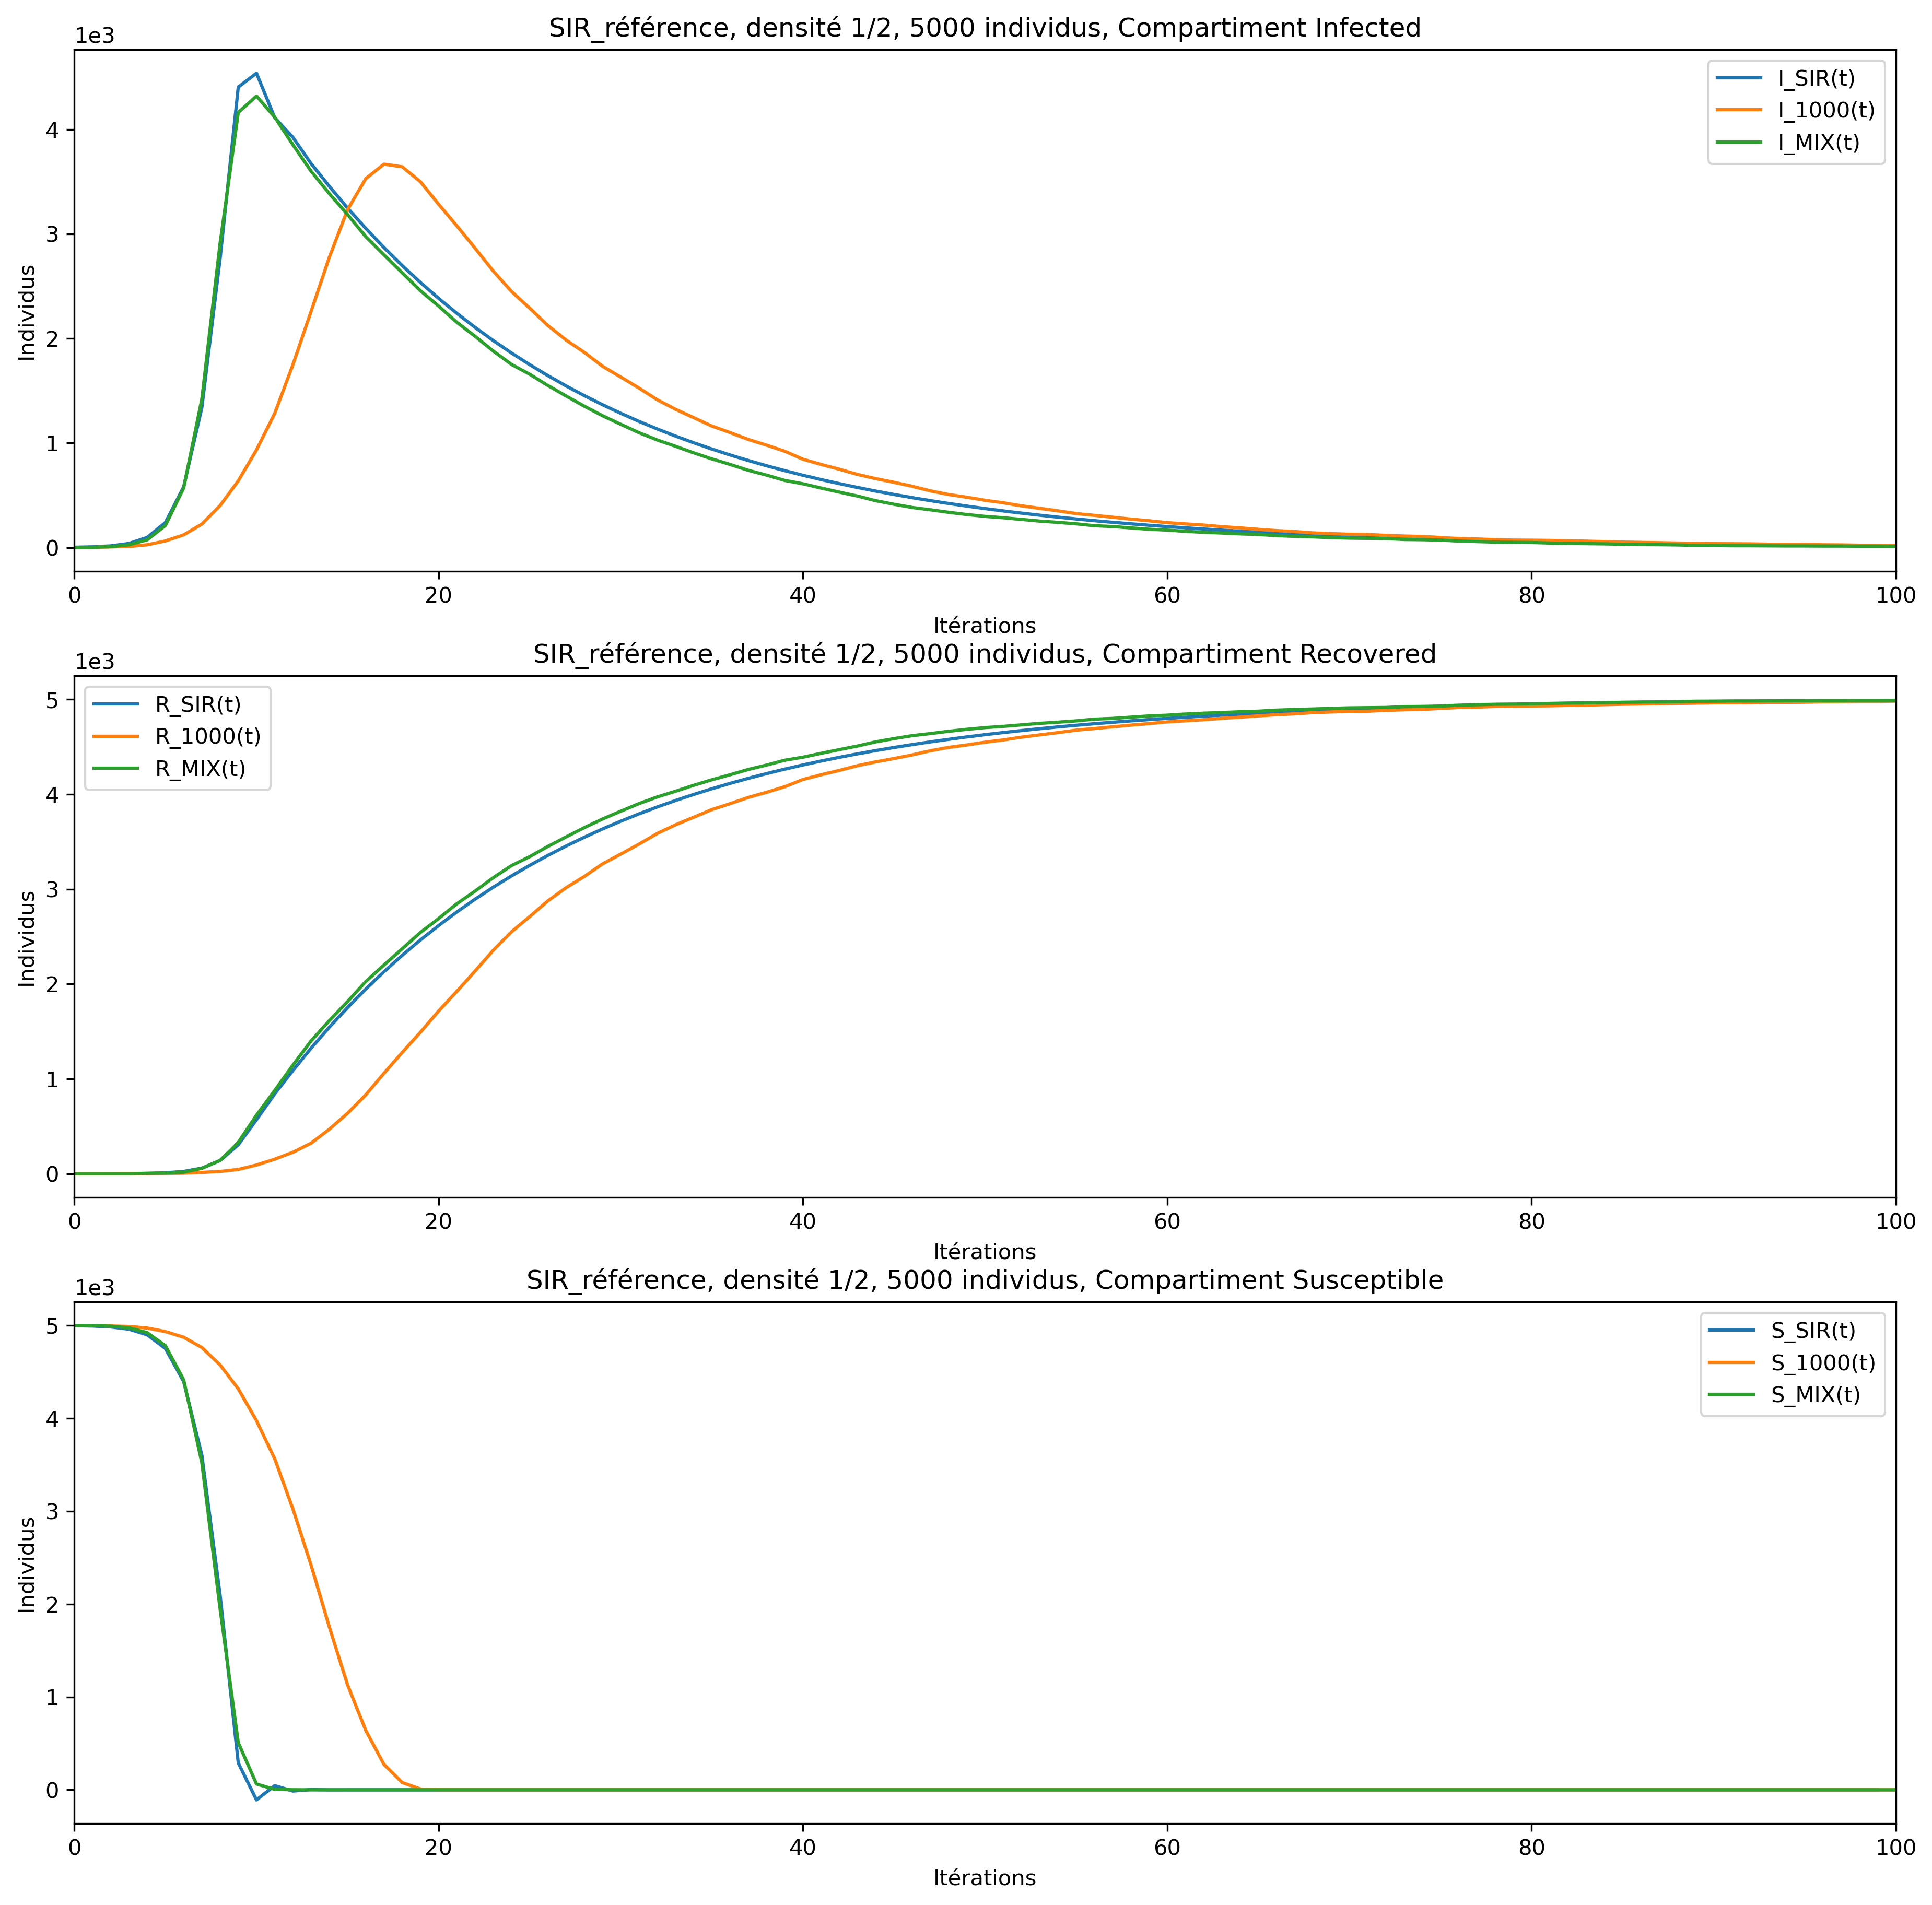
\includegraphics[width=.4\textwidth]{Images/SIR_ref_2_5.png}
	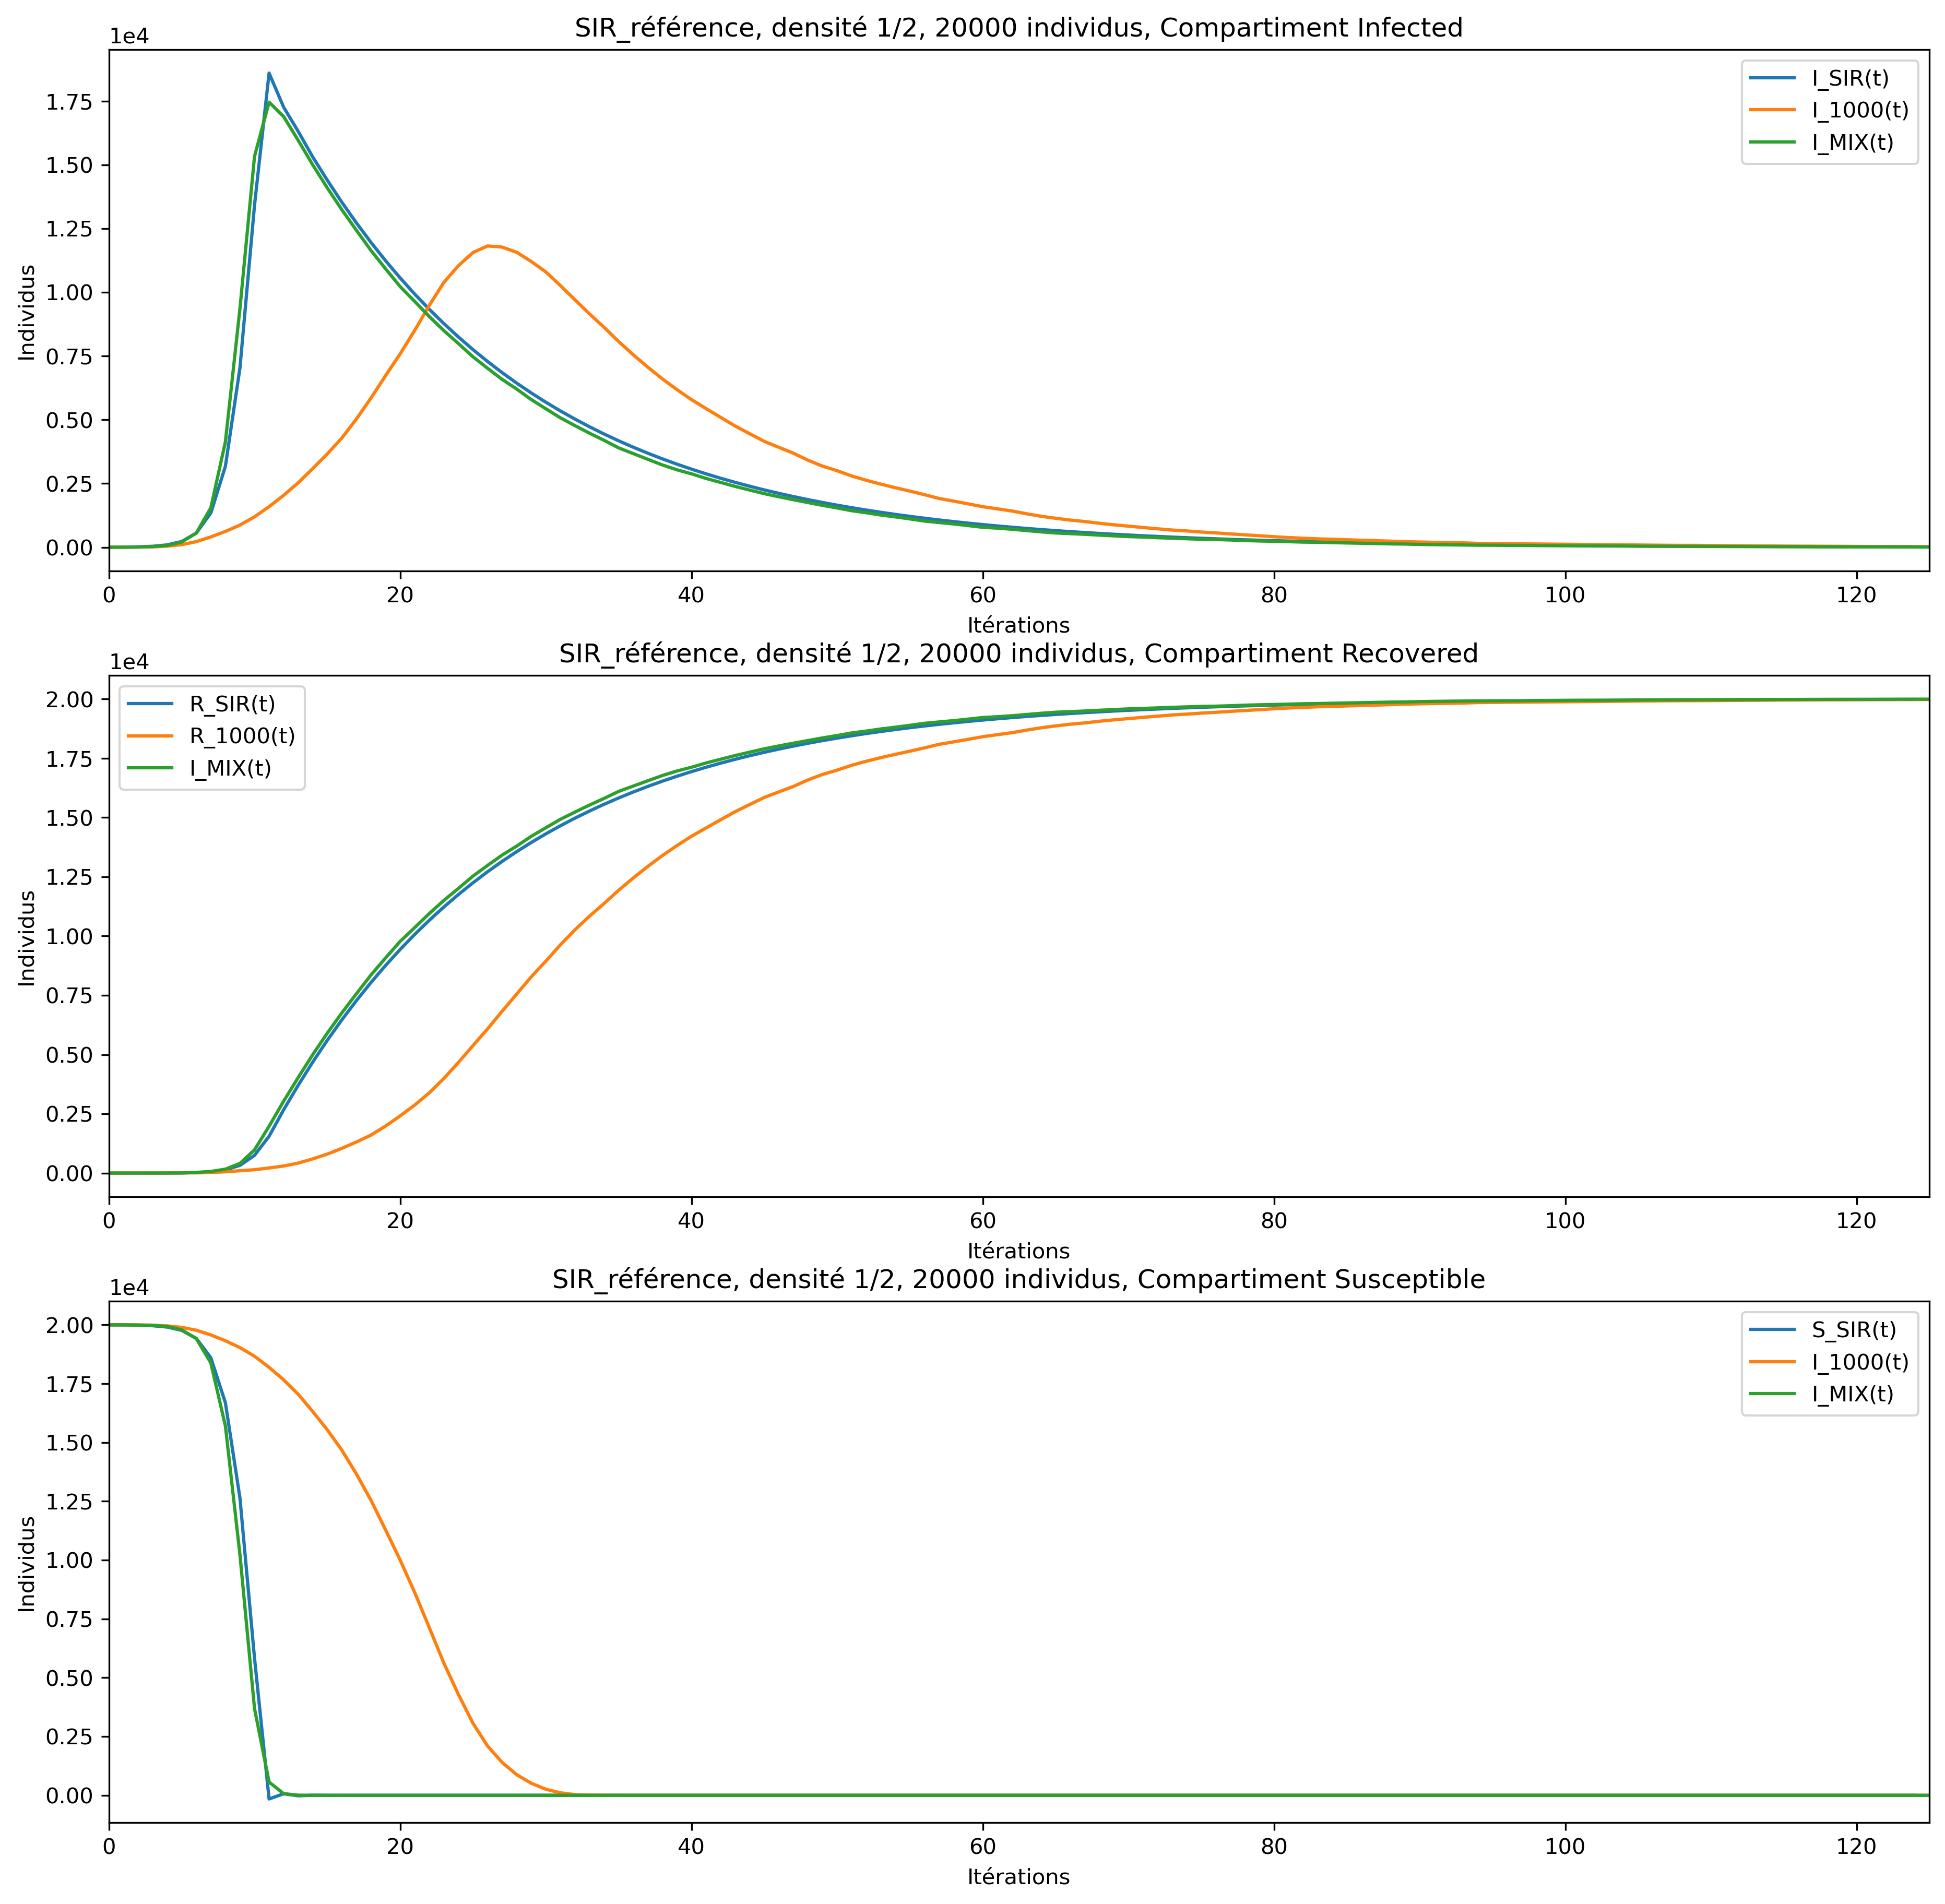
\includegraphics[width=.4\textwidth]{Images/SIR_ref_2_20.png}
	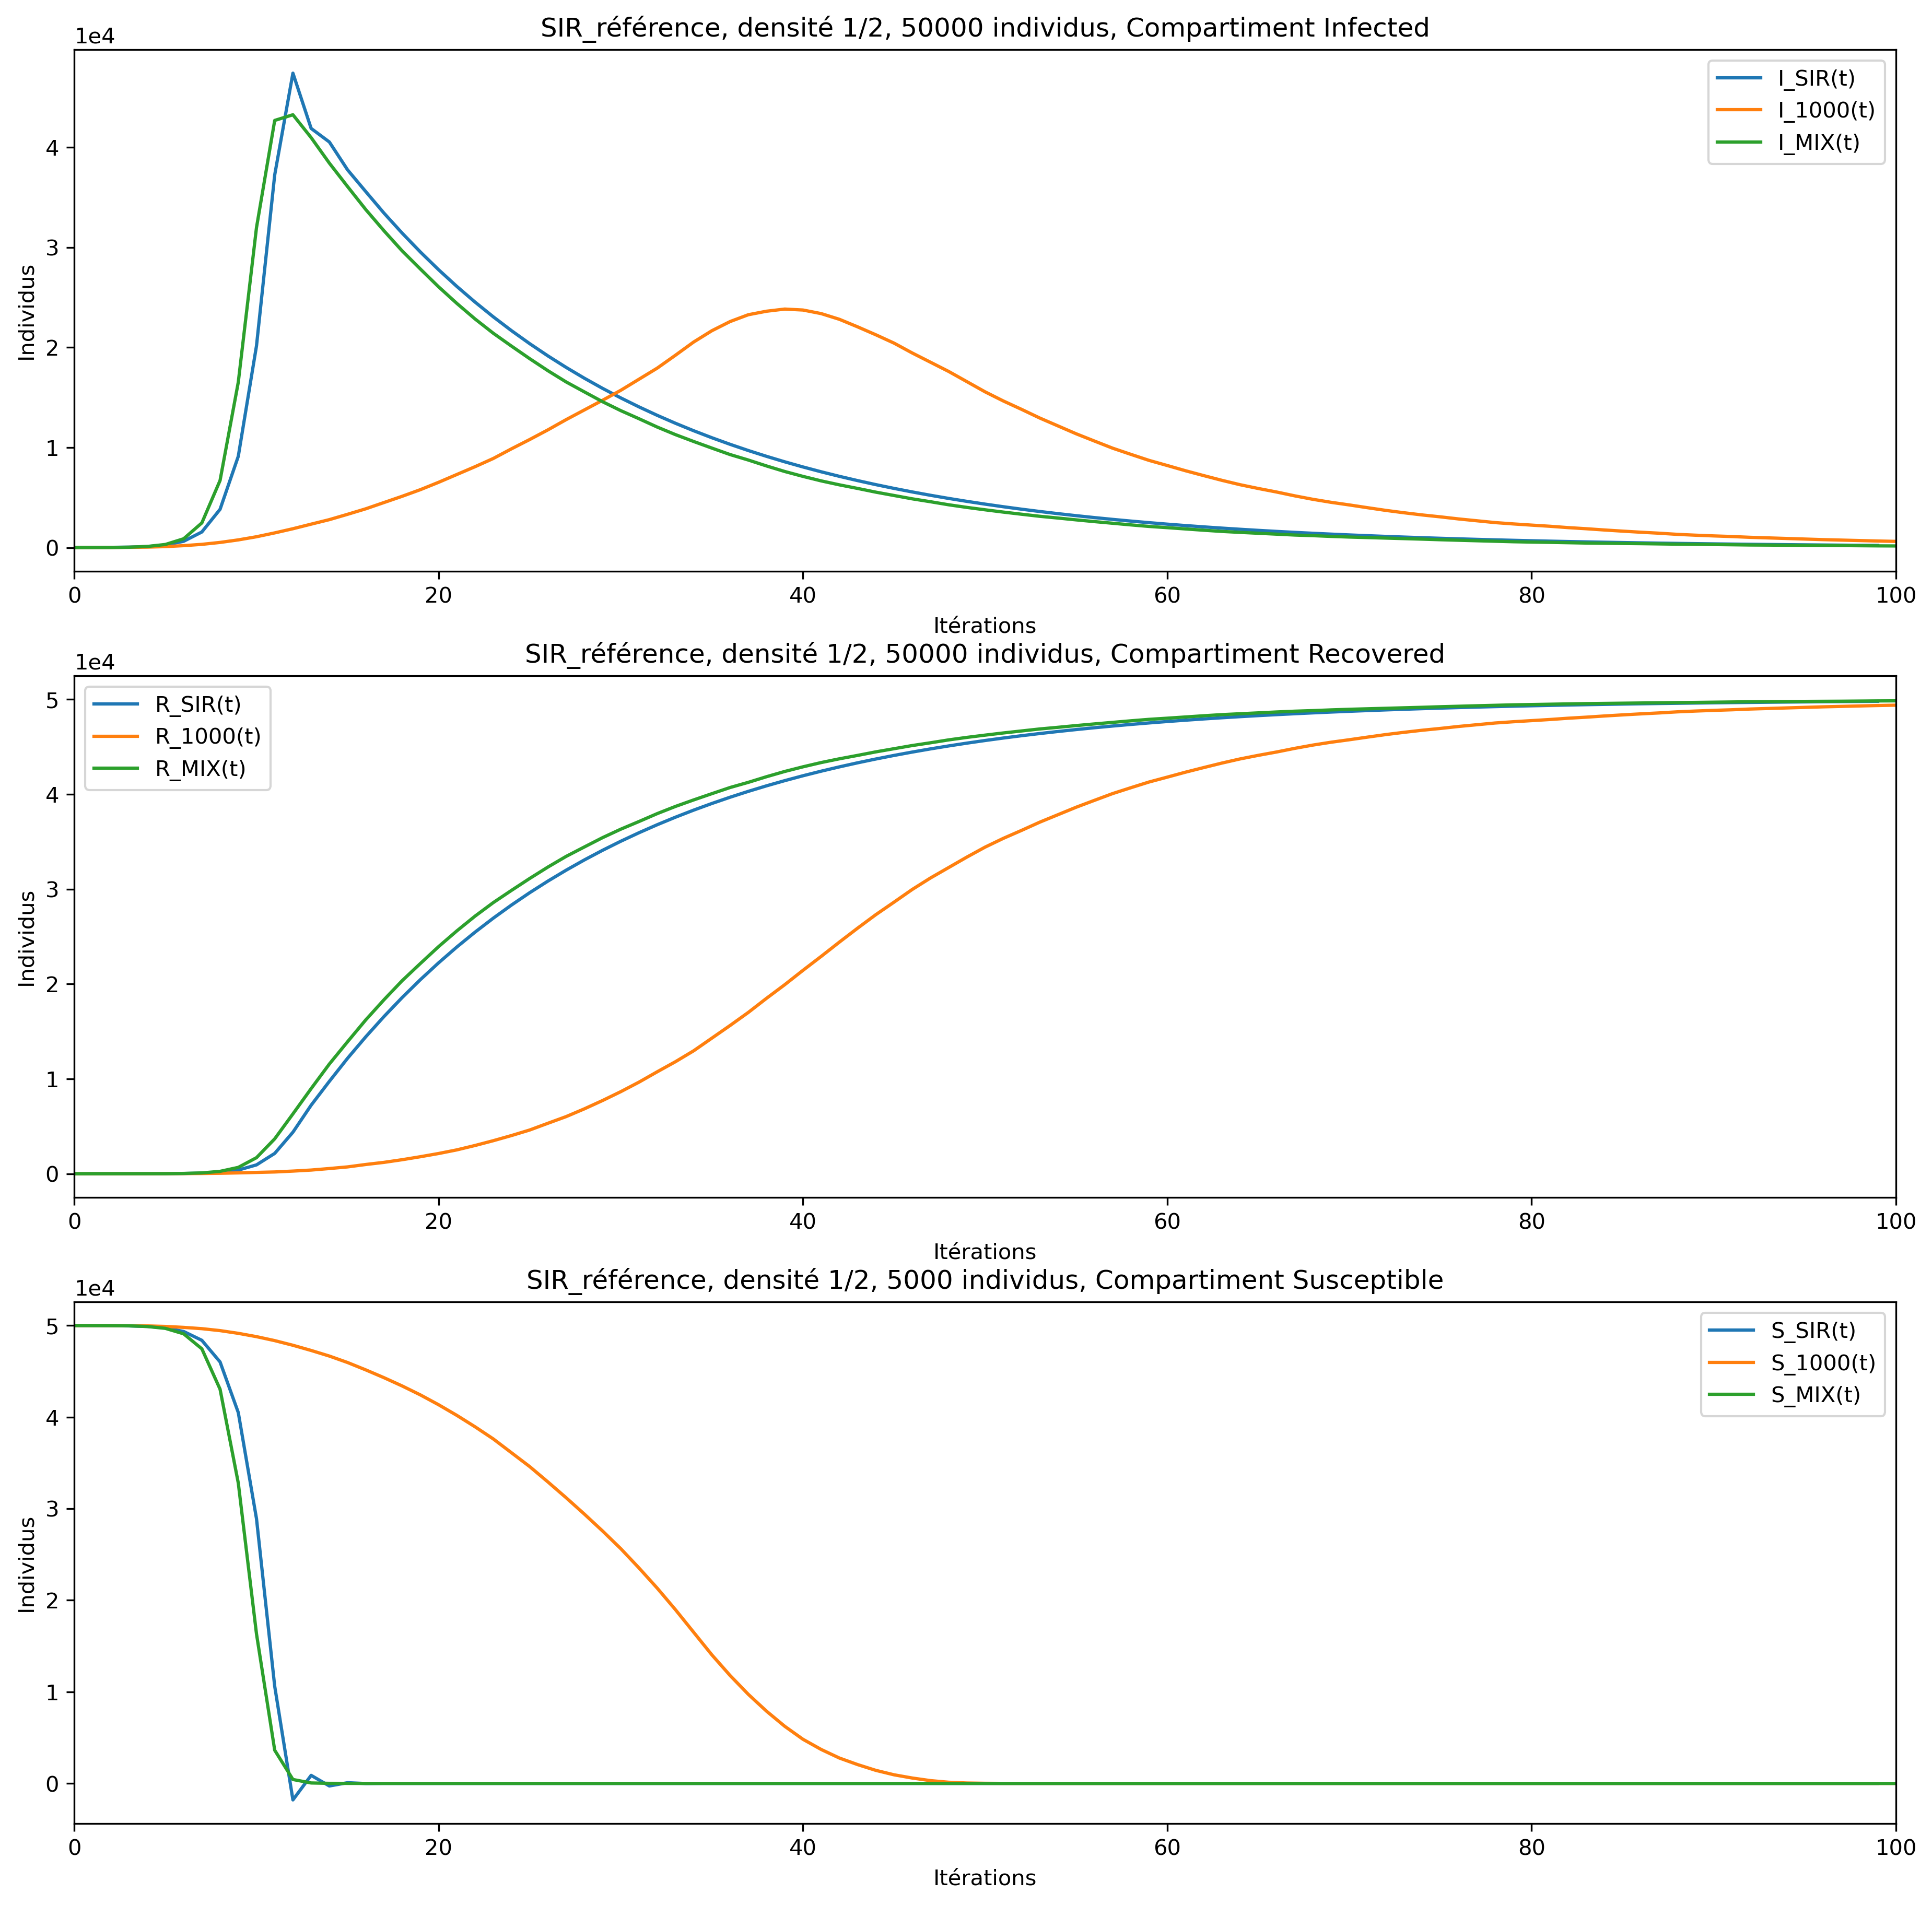
\includegraphics[width=.4\textwidth]{Images/SIR_ref_2_50.png}
	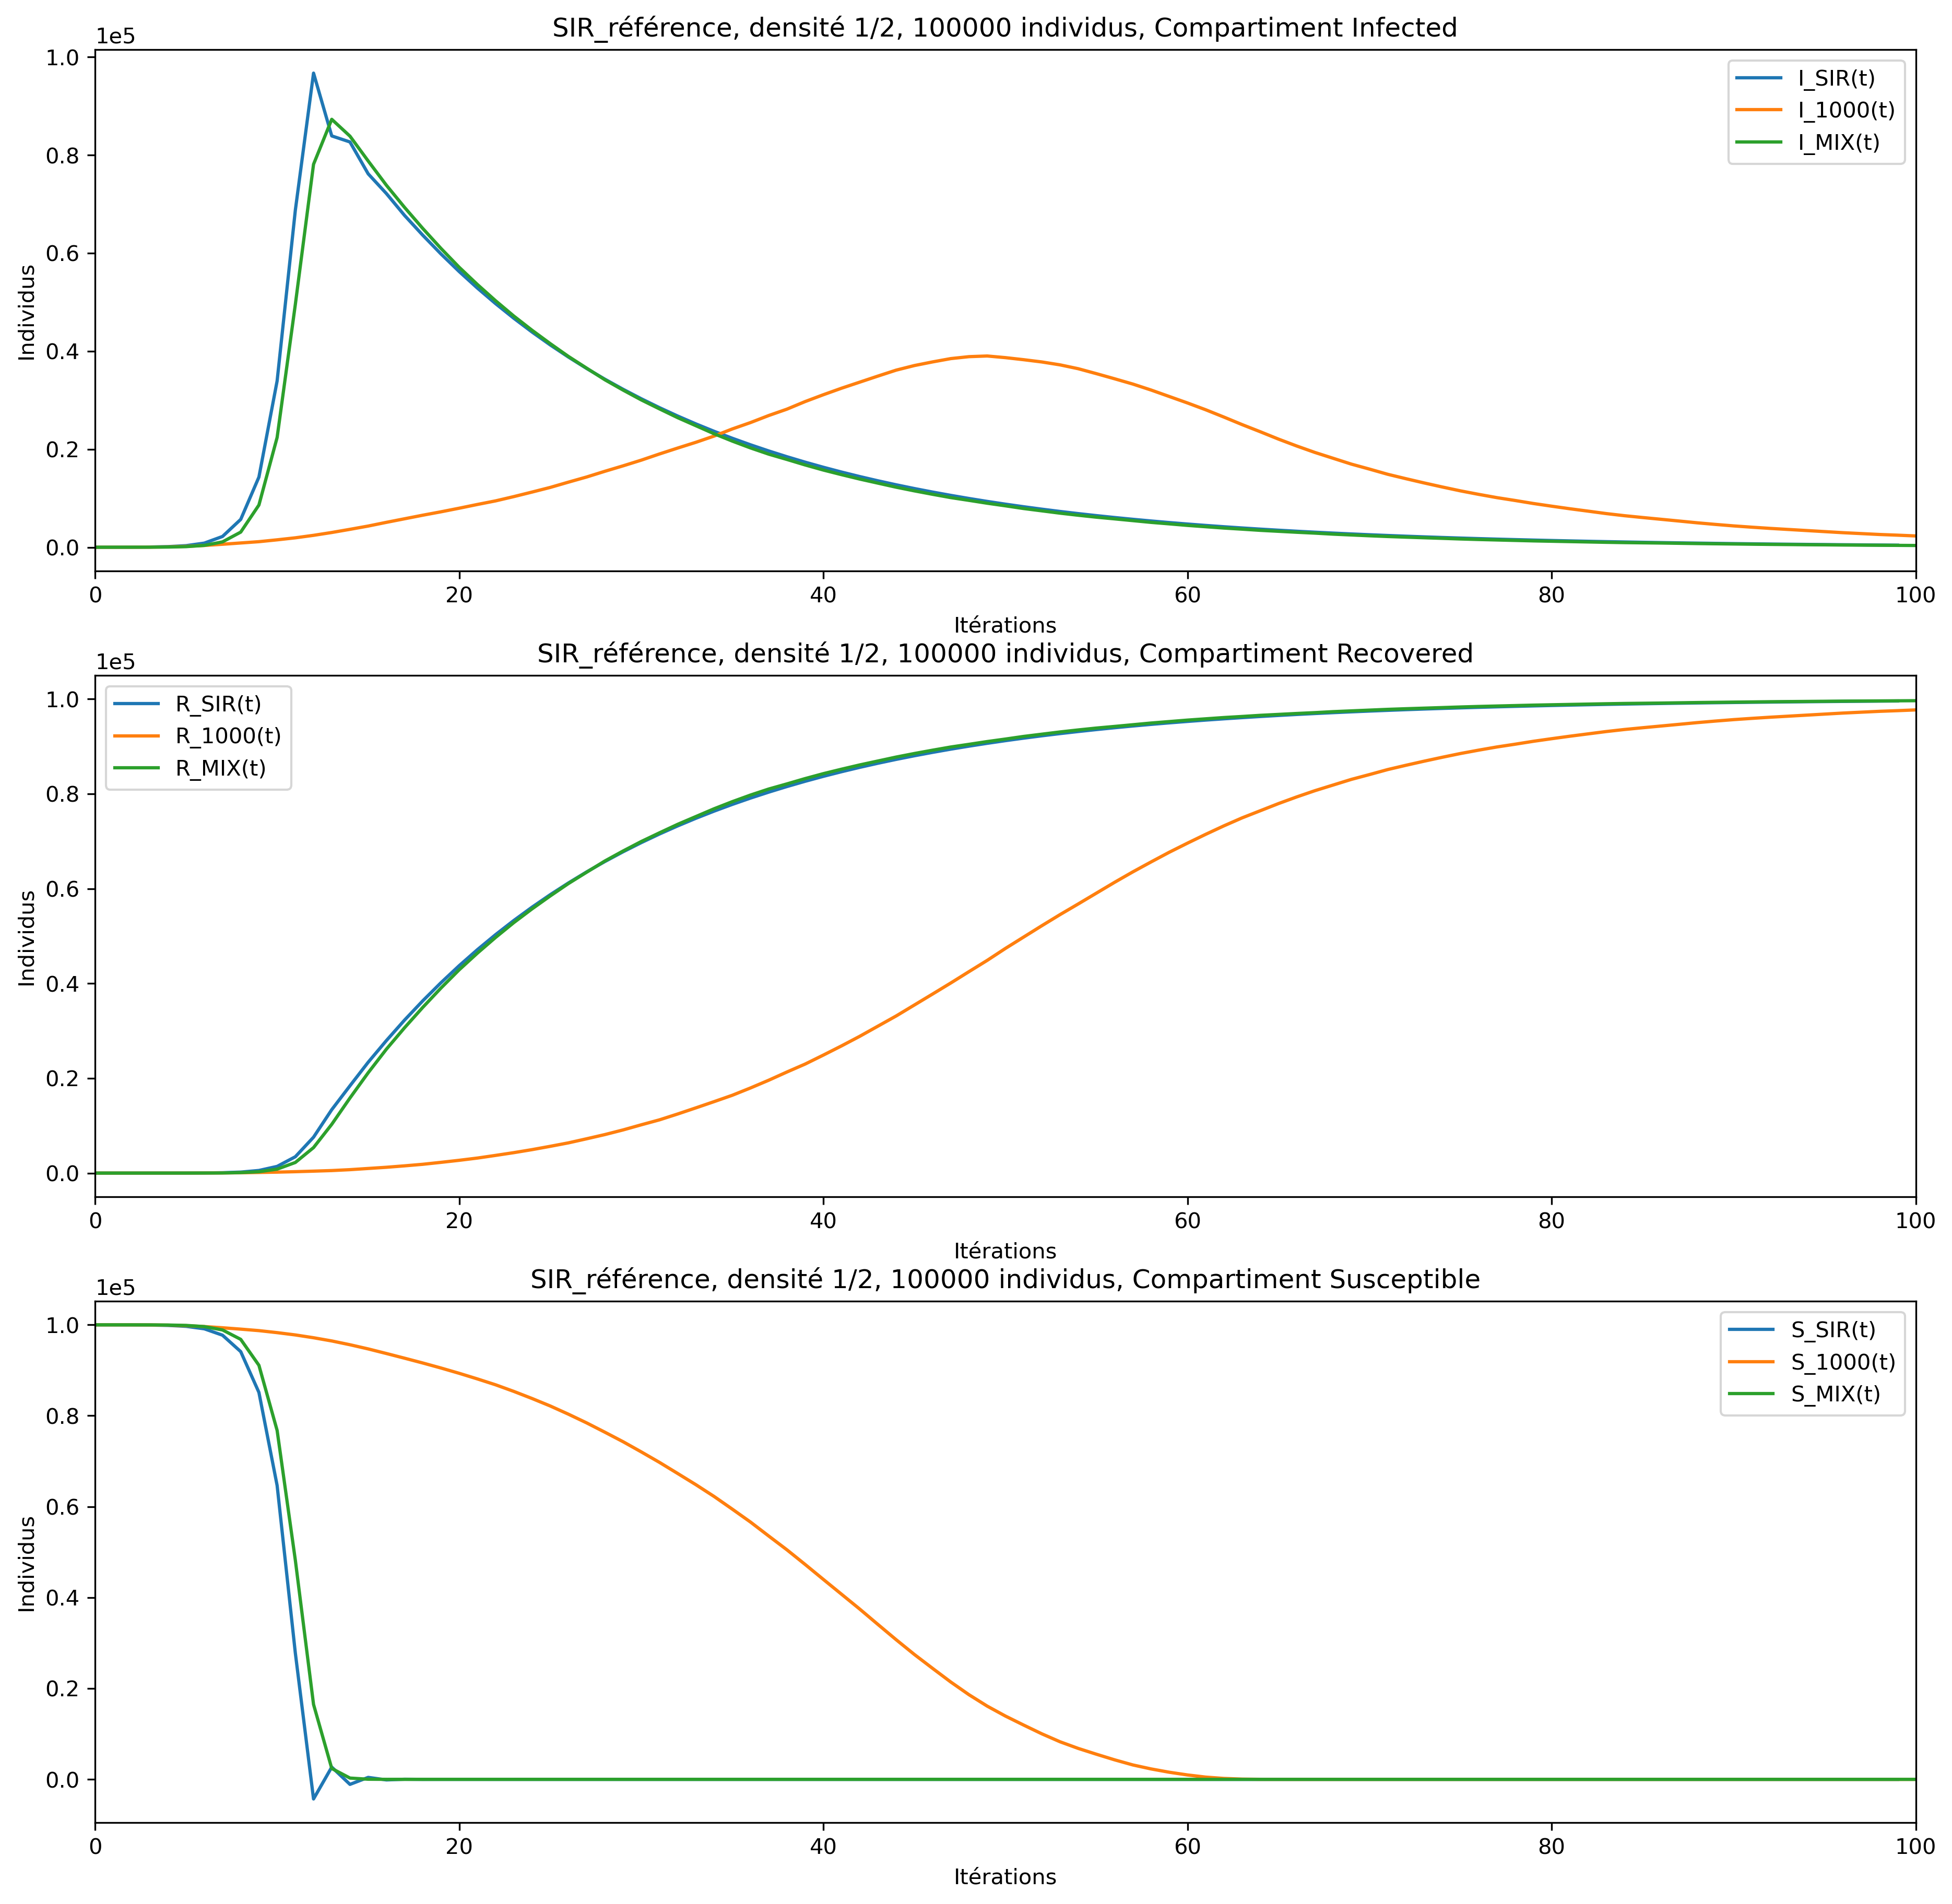
\includegraphics[width=.4\textwidth]{Images/SIR_ref_2_100.png}
	\caption{test}
\end{figure}

Pour les systèmes de forte densité, les simulations aux $1000$ mouvements peinent à se mélanger. Par conséquent, les événements sont plus tardifs. Nous pouvons observer les mêmes comportements que pour les simulations SI.

\newpage

\begin{figure}[h]
	\centering
	\captionsetup{justification=centering}
	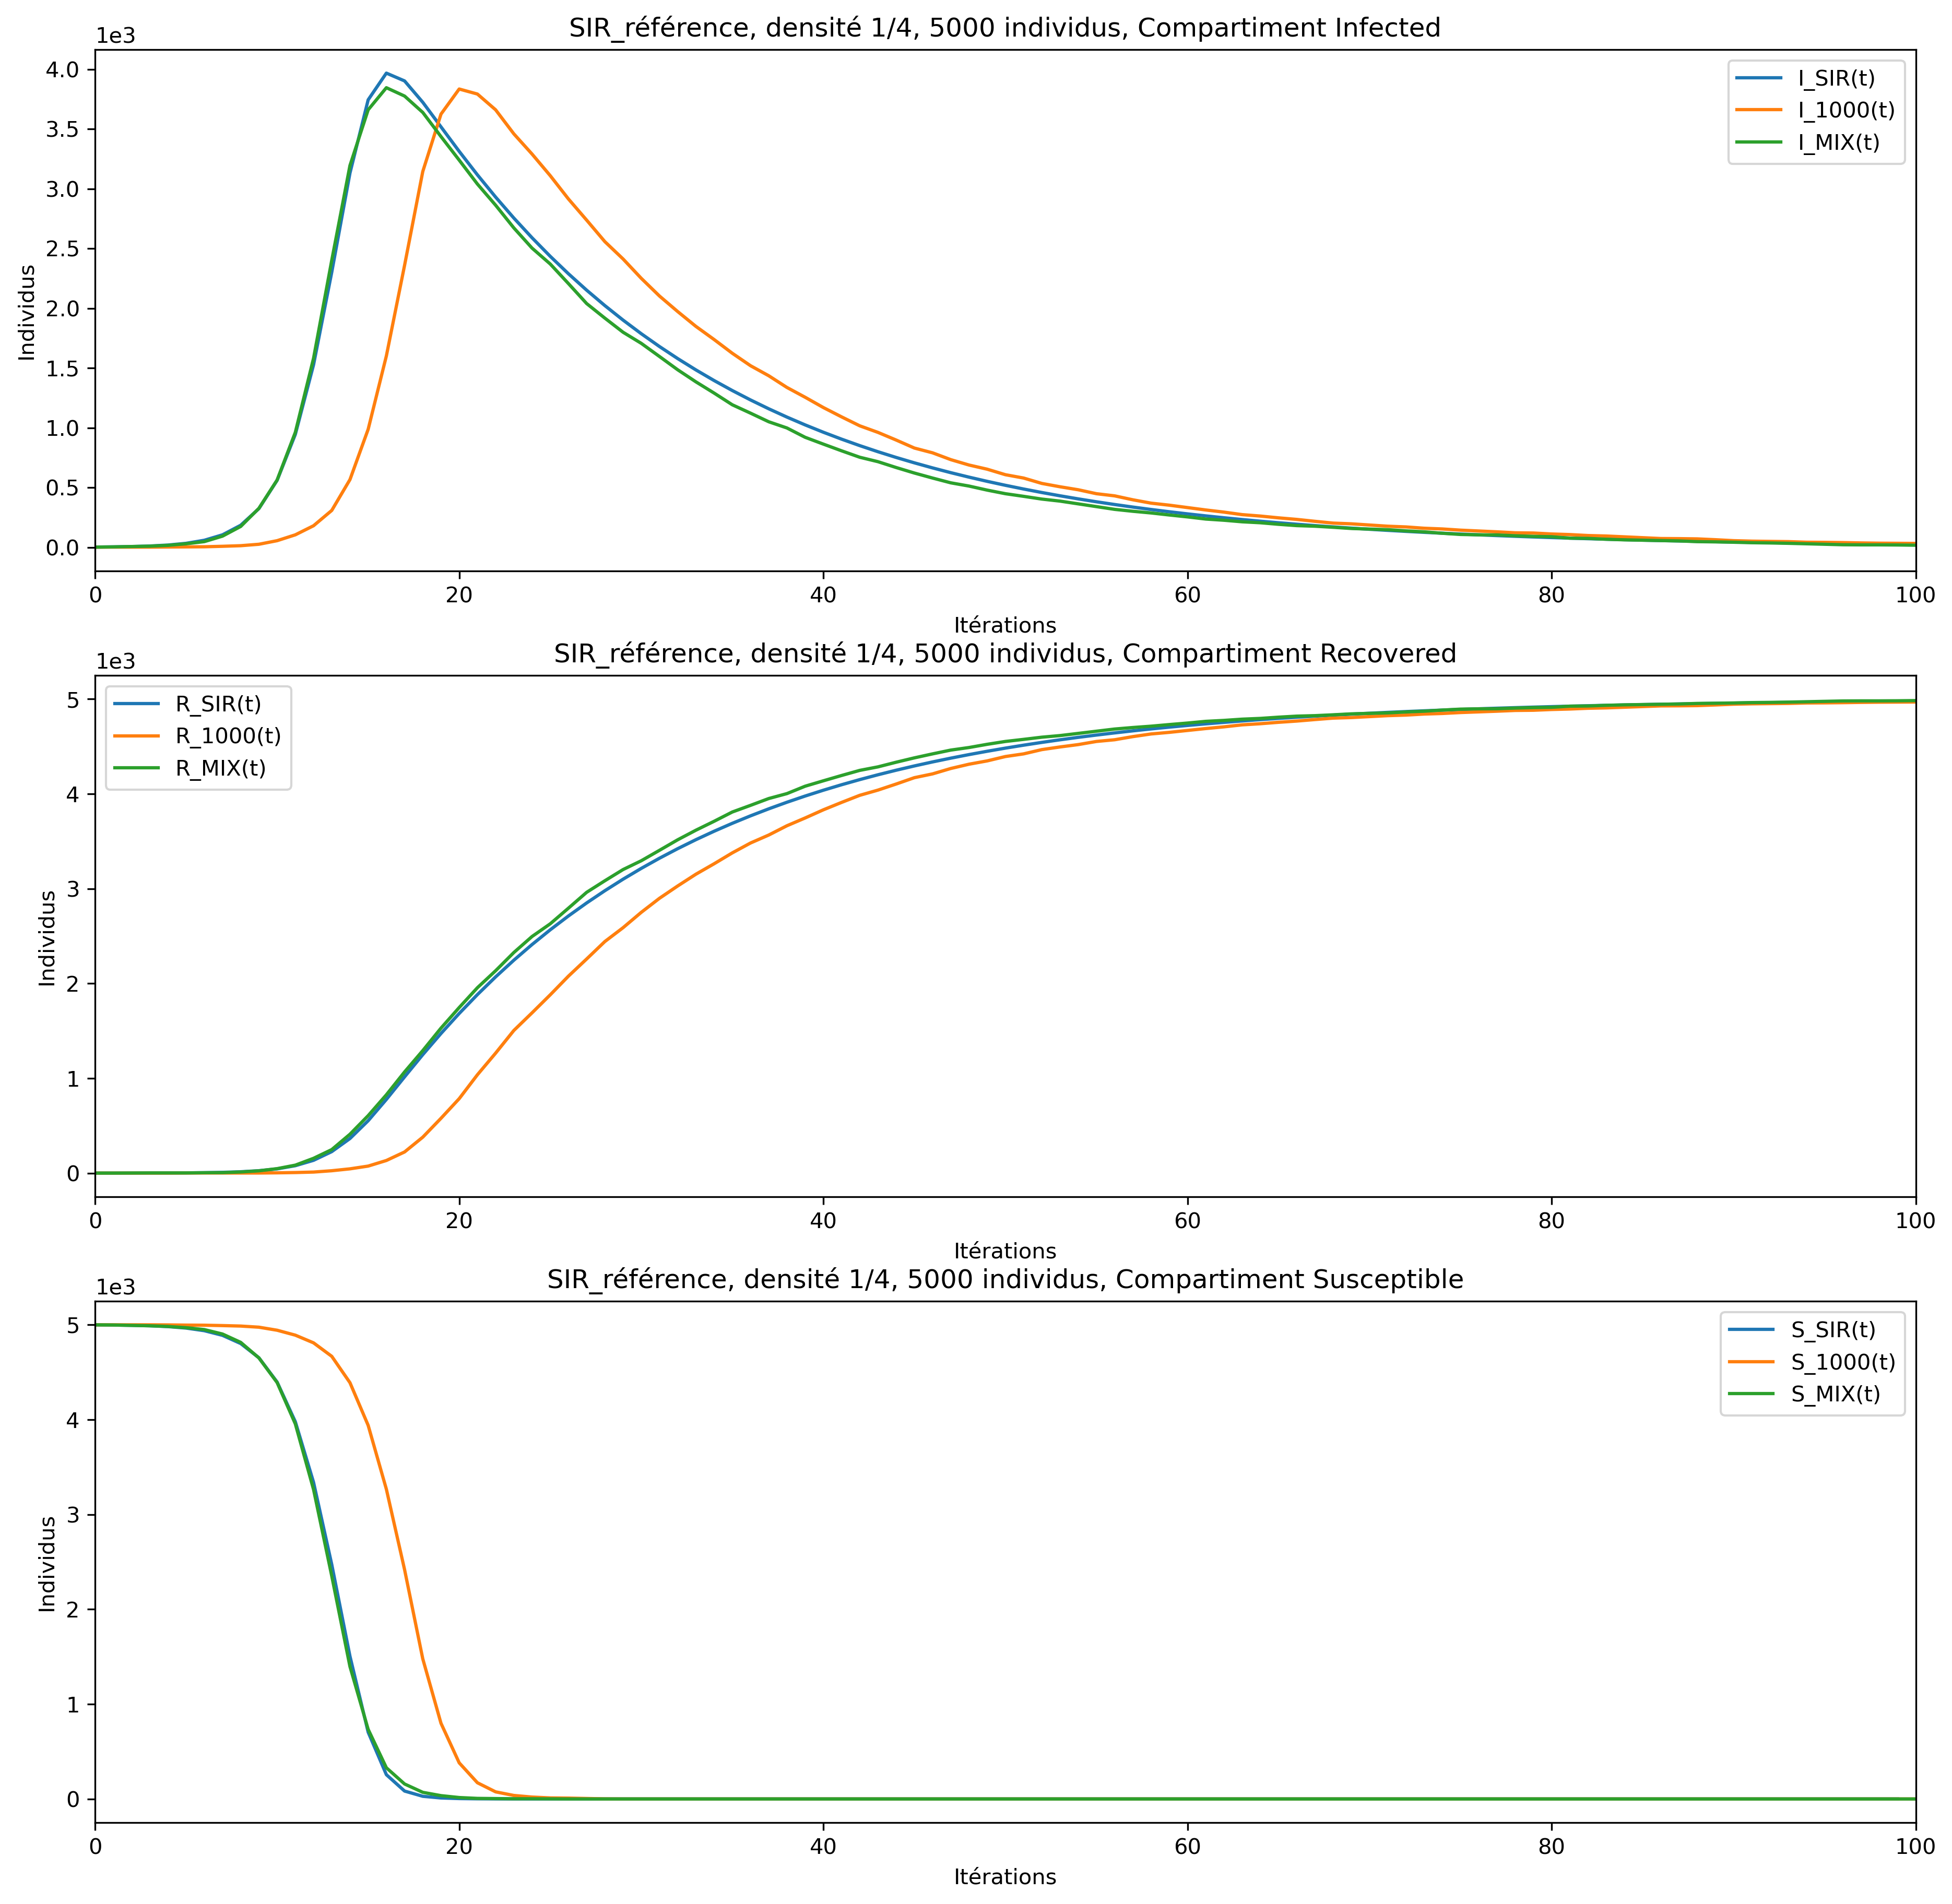
\includegraphics[width=.4\textwidth]{Images/SIR_ref_4_5.png}
	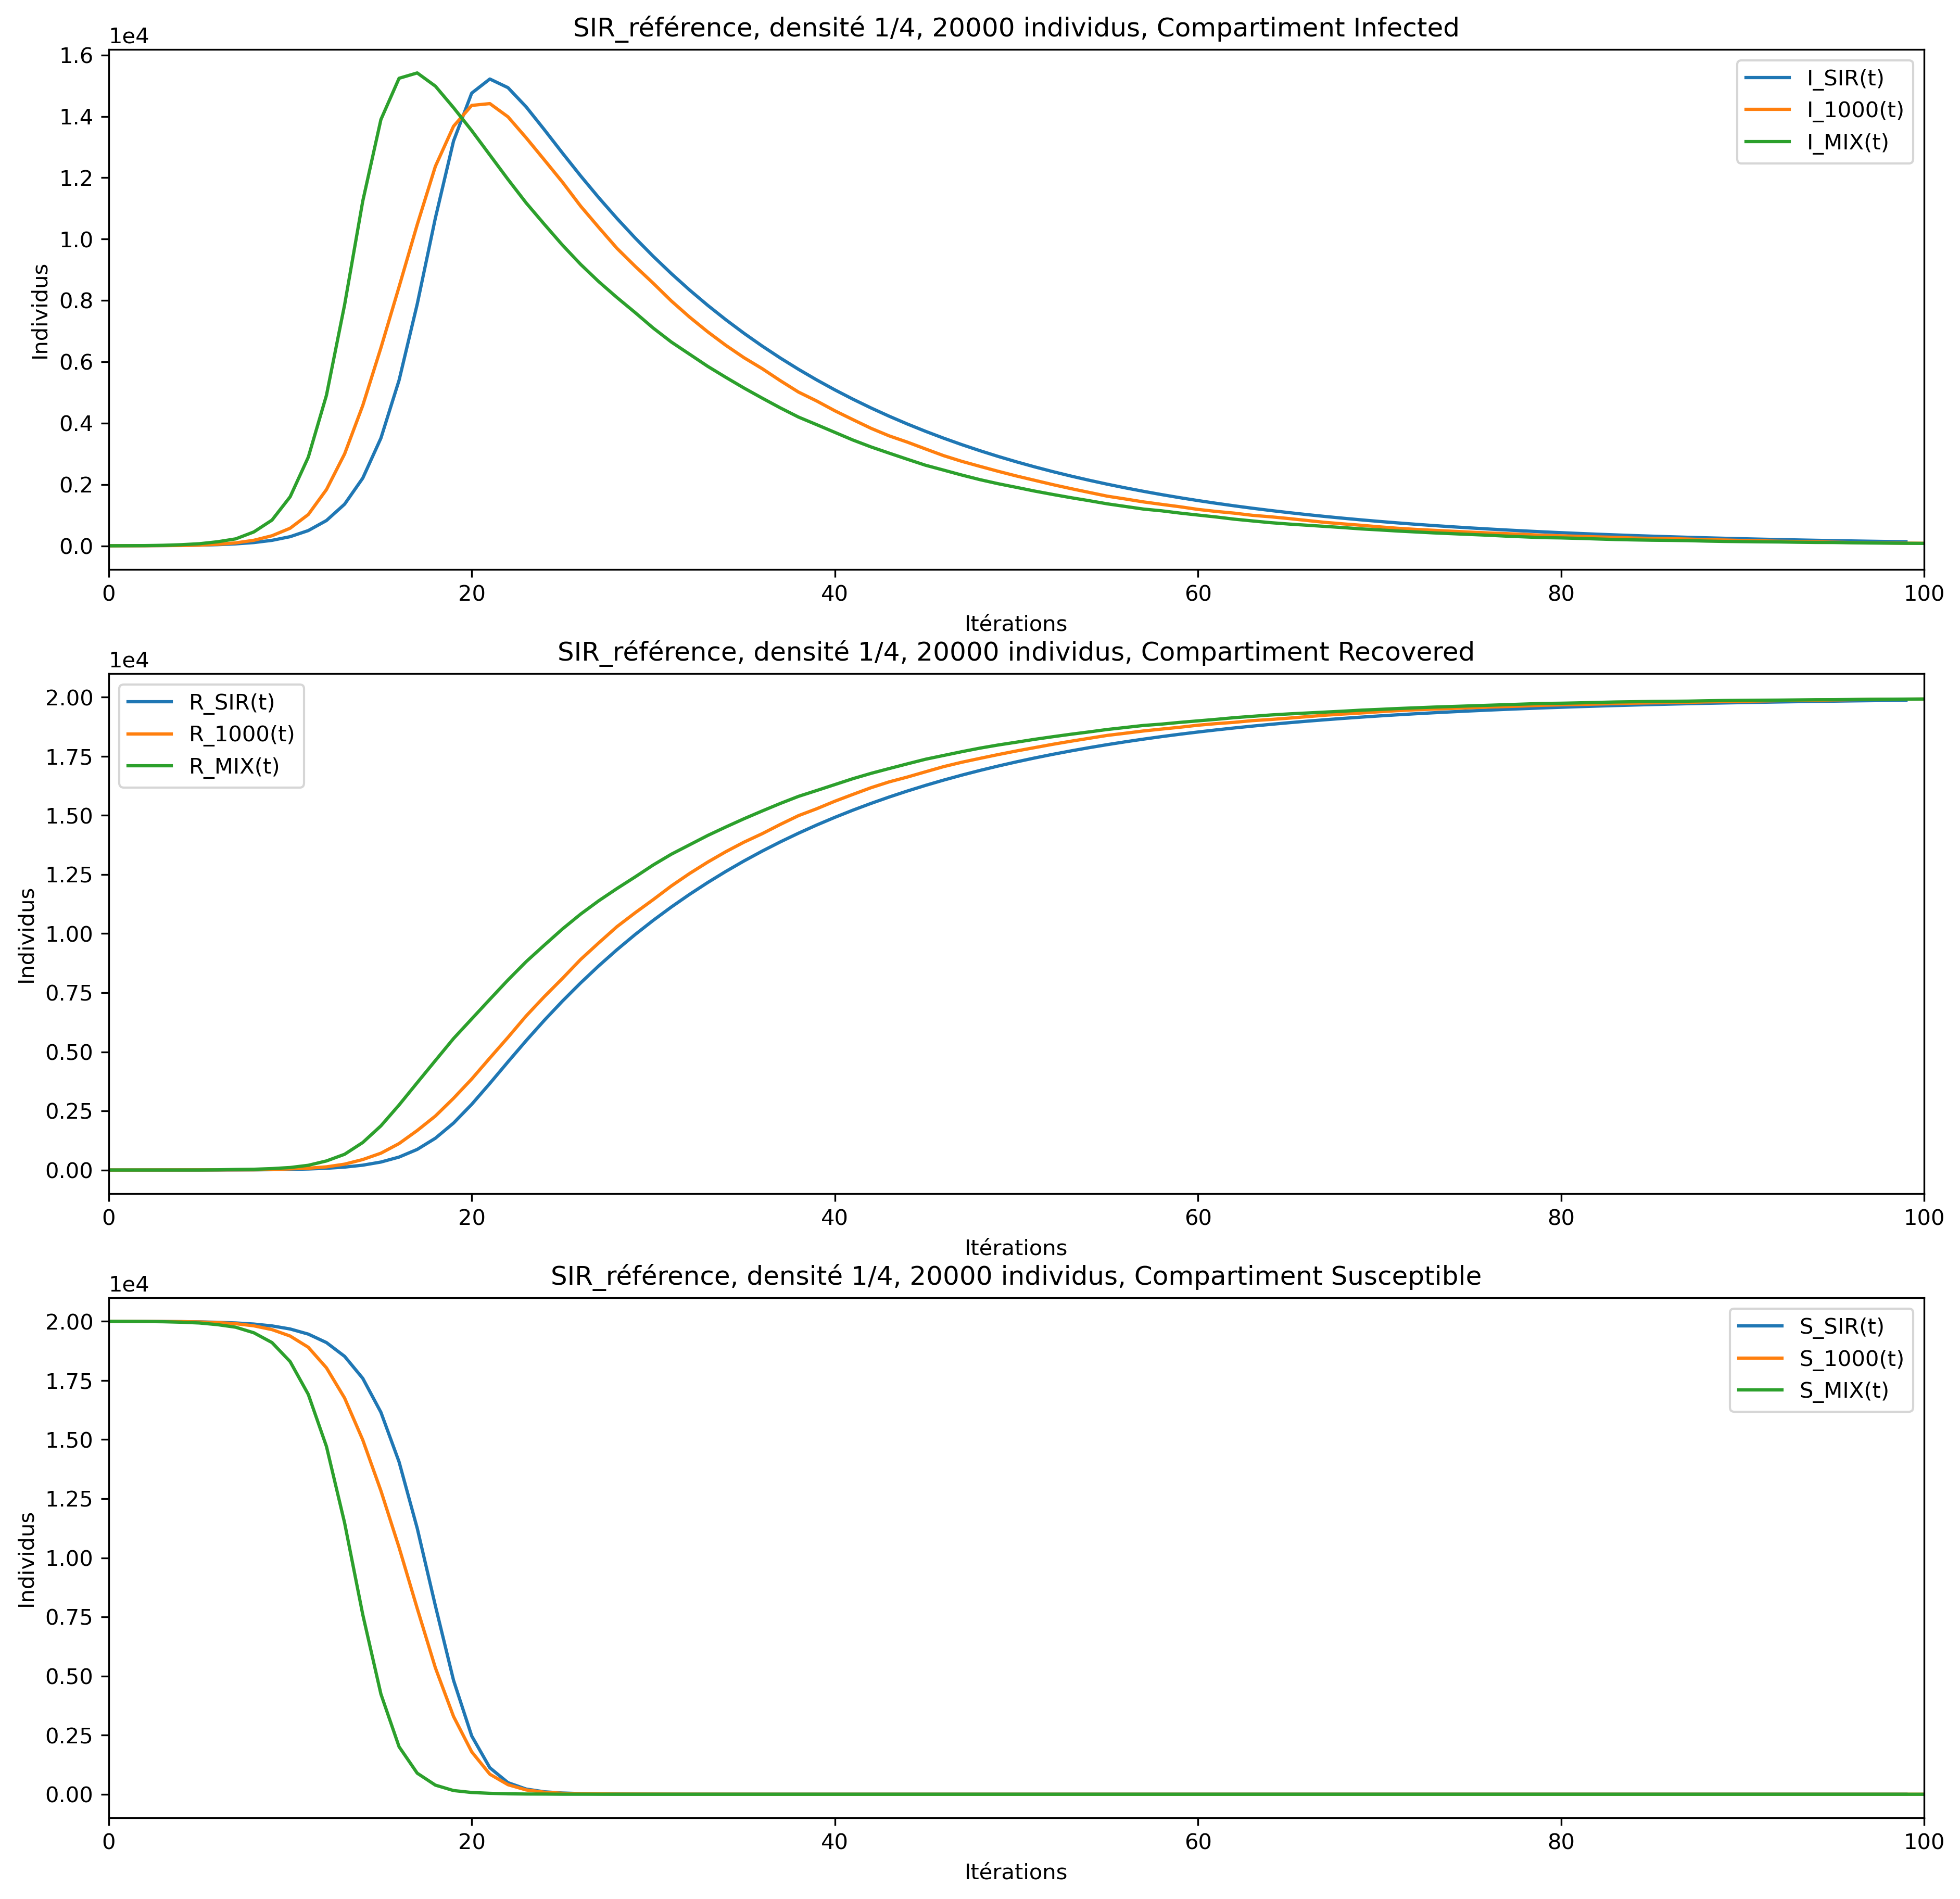
\includegraphics[width=.4\textwidth]{Images/SIR_ref_4_20.png}
	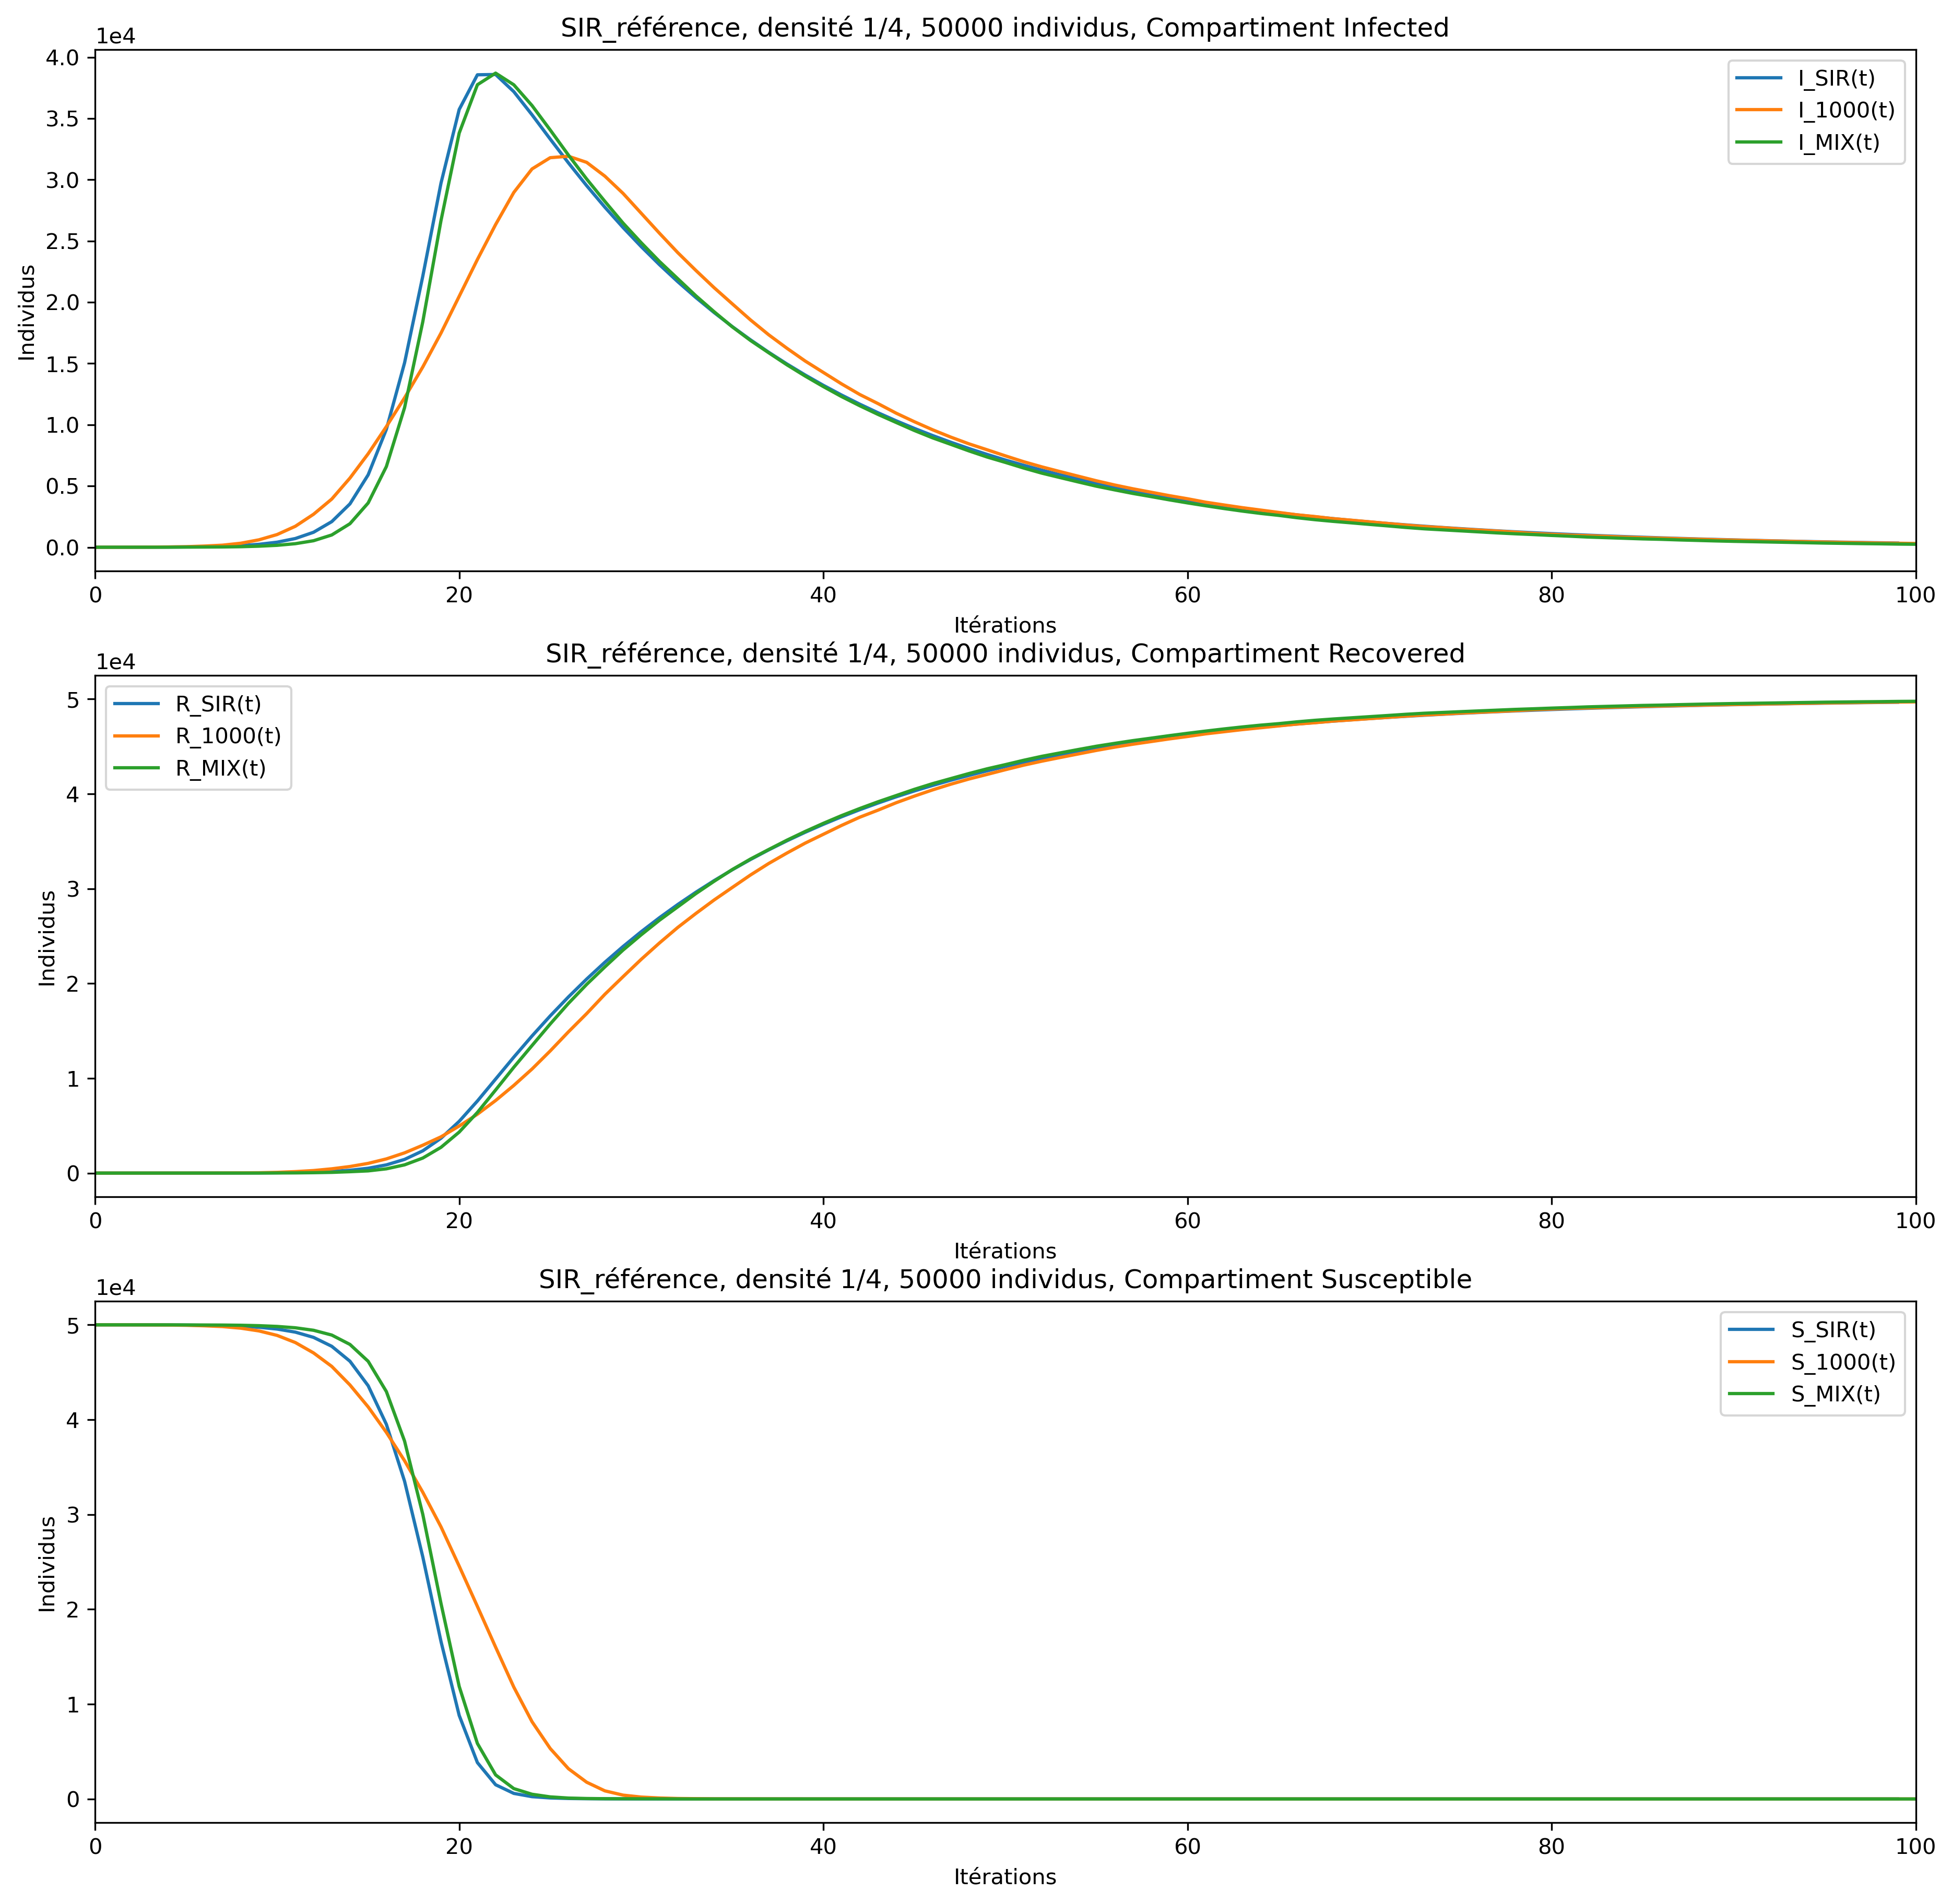
\includegraphics[width=.4\textwidth]{Images/SIR_ref_4_50.png}
	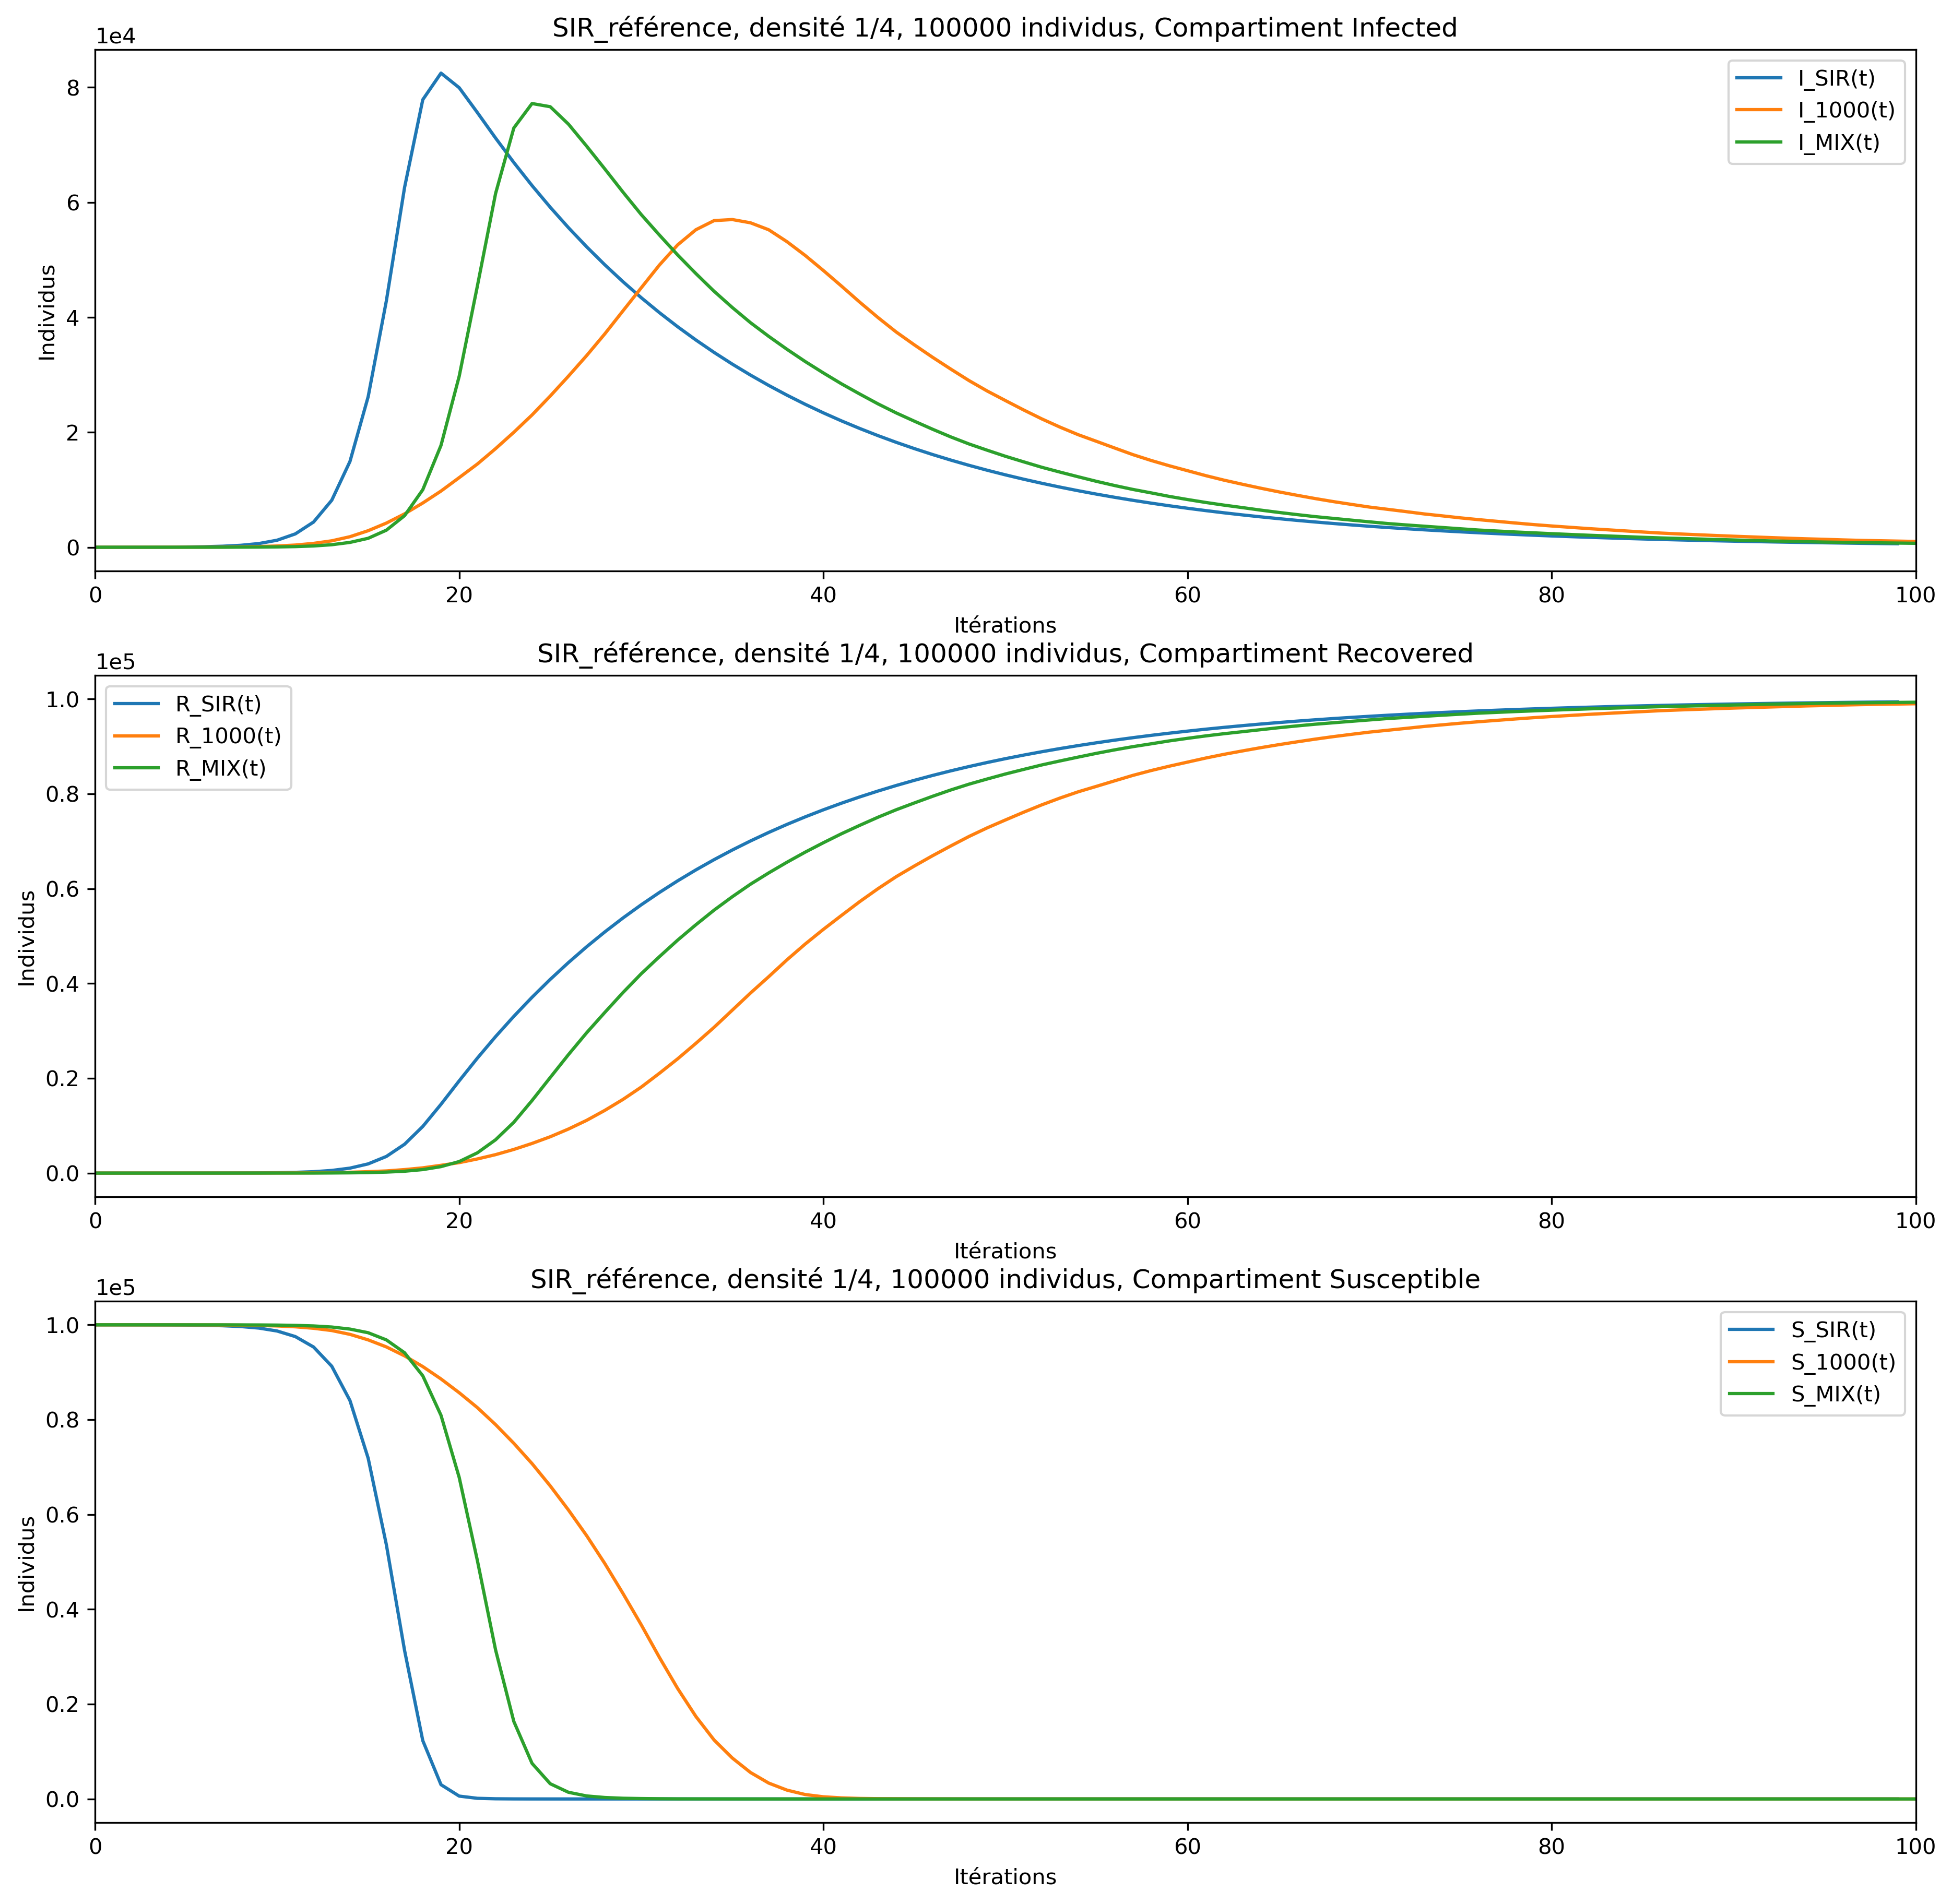
\includegraphics[width=.4\textwidth]{Images/SIR_ref_4_100.png}
	\caption{test}
\end{figure}

En densité $\frac{1}{4}$ les simulations des $1000$ mouvements tendent d'avantage vers le mélange parfait. Les courbes sont toujours plus progressives et donc les événements plus lents.

\newpage

\begin{figure}[h]
	\centering
	\captionsetup{justification=centering}
	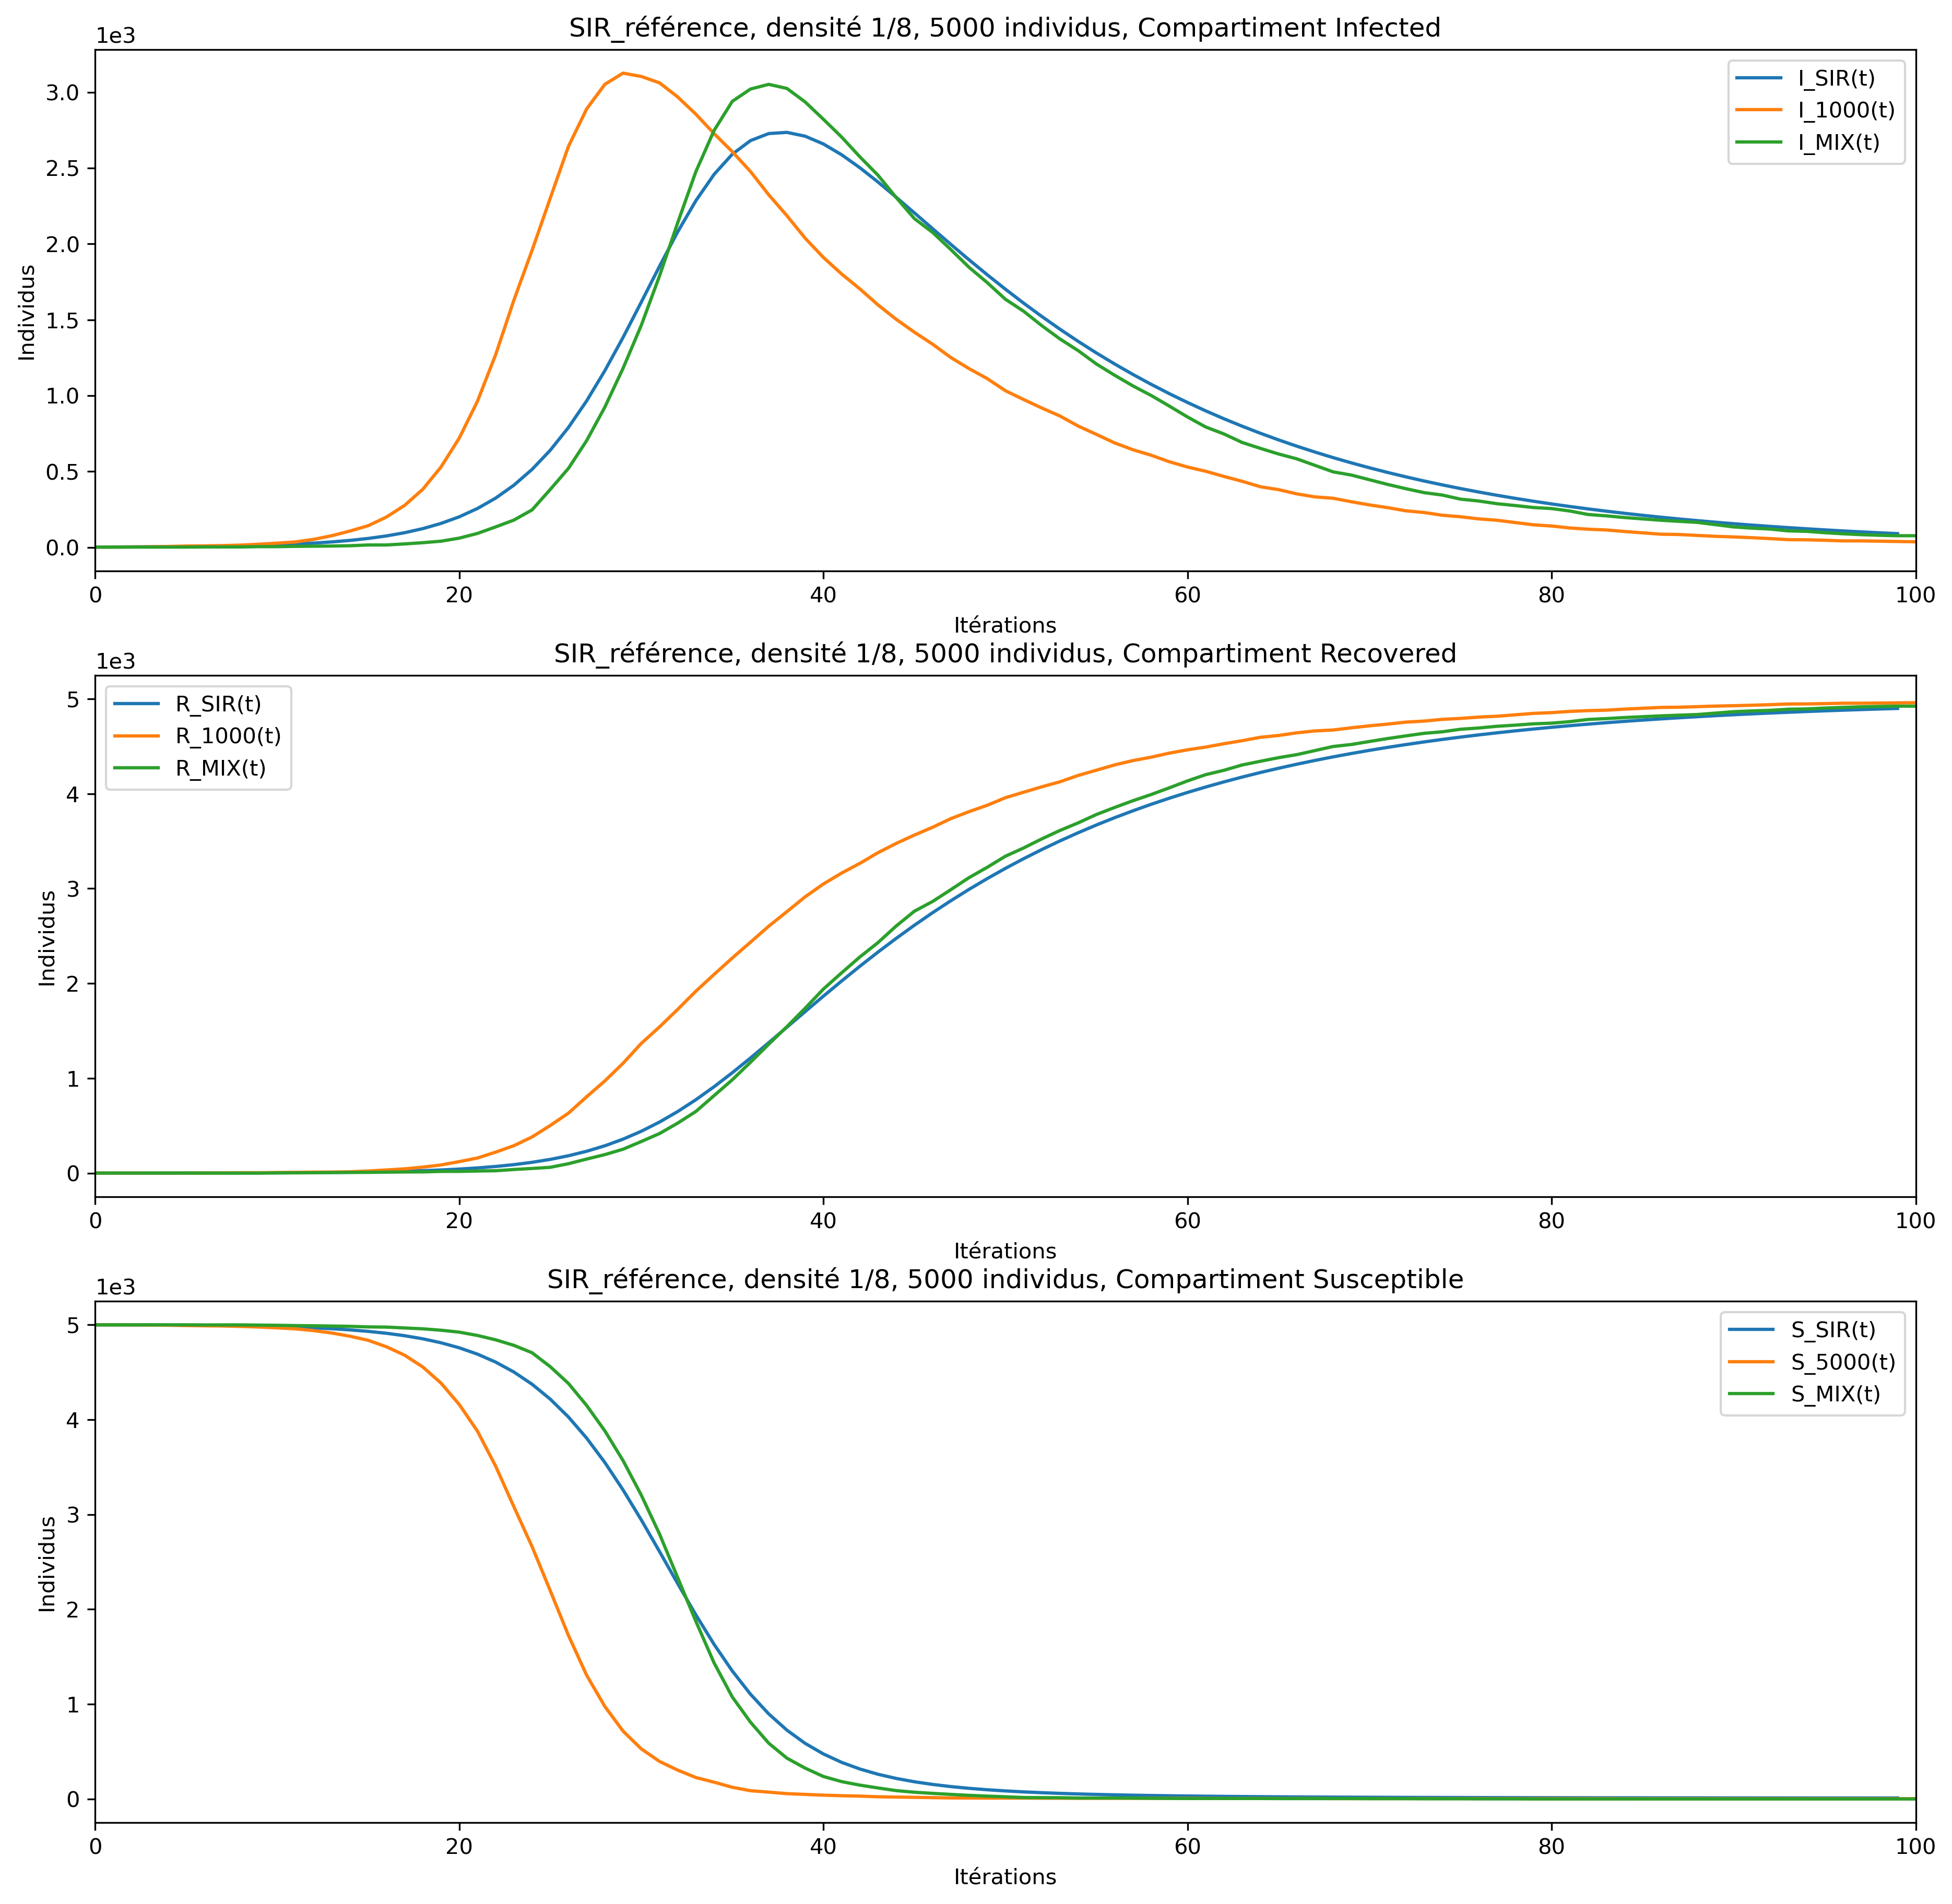
\includegraphics[width=.4\textwidth]{Images/SIR_ref_8_5.png}
	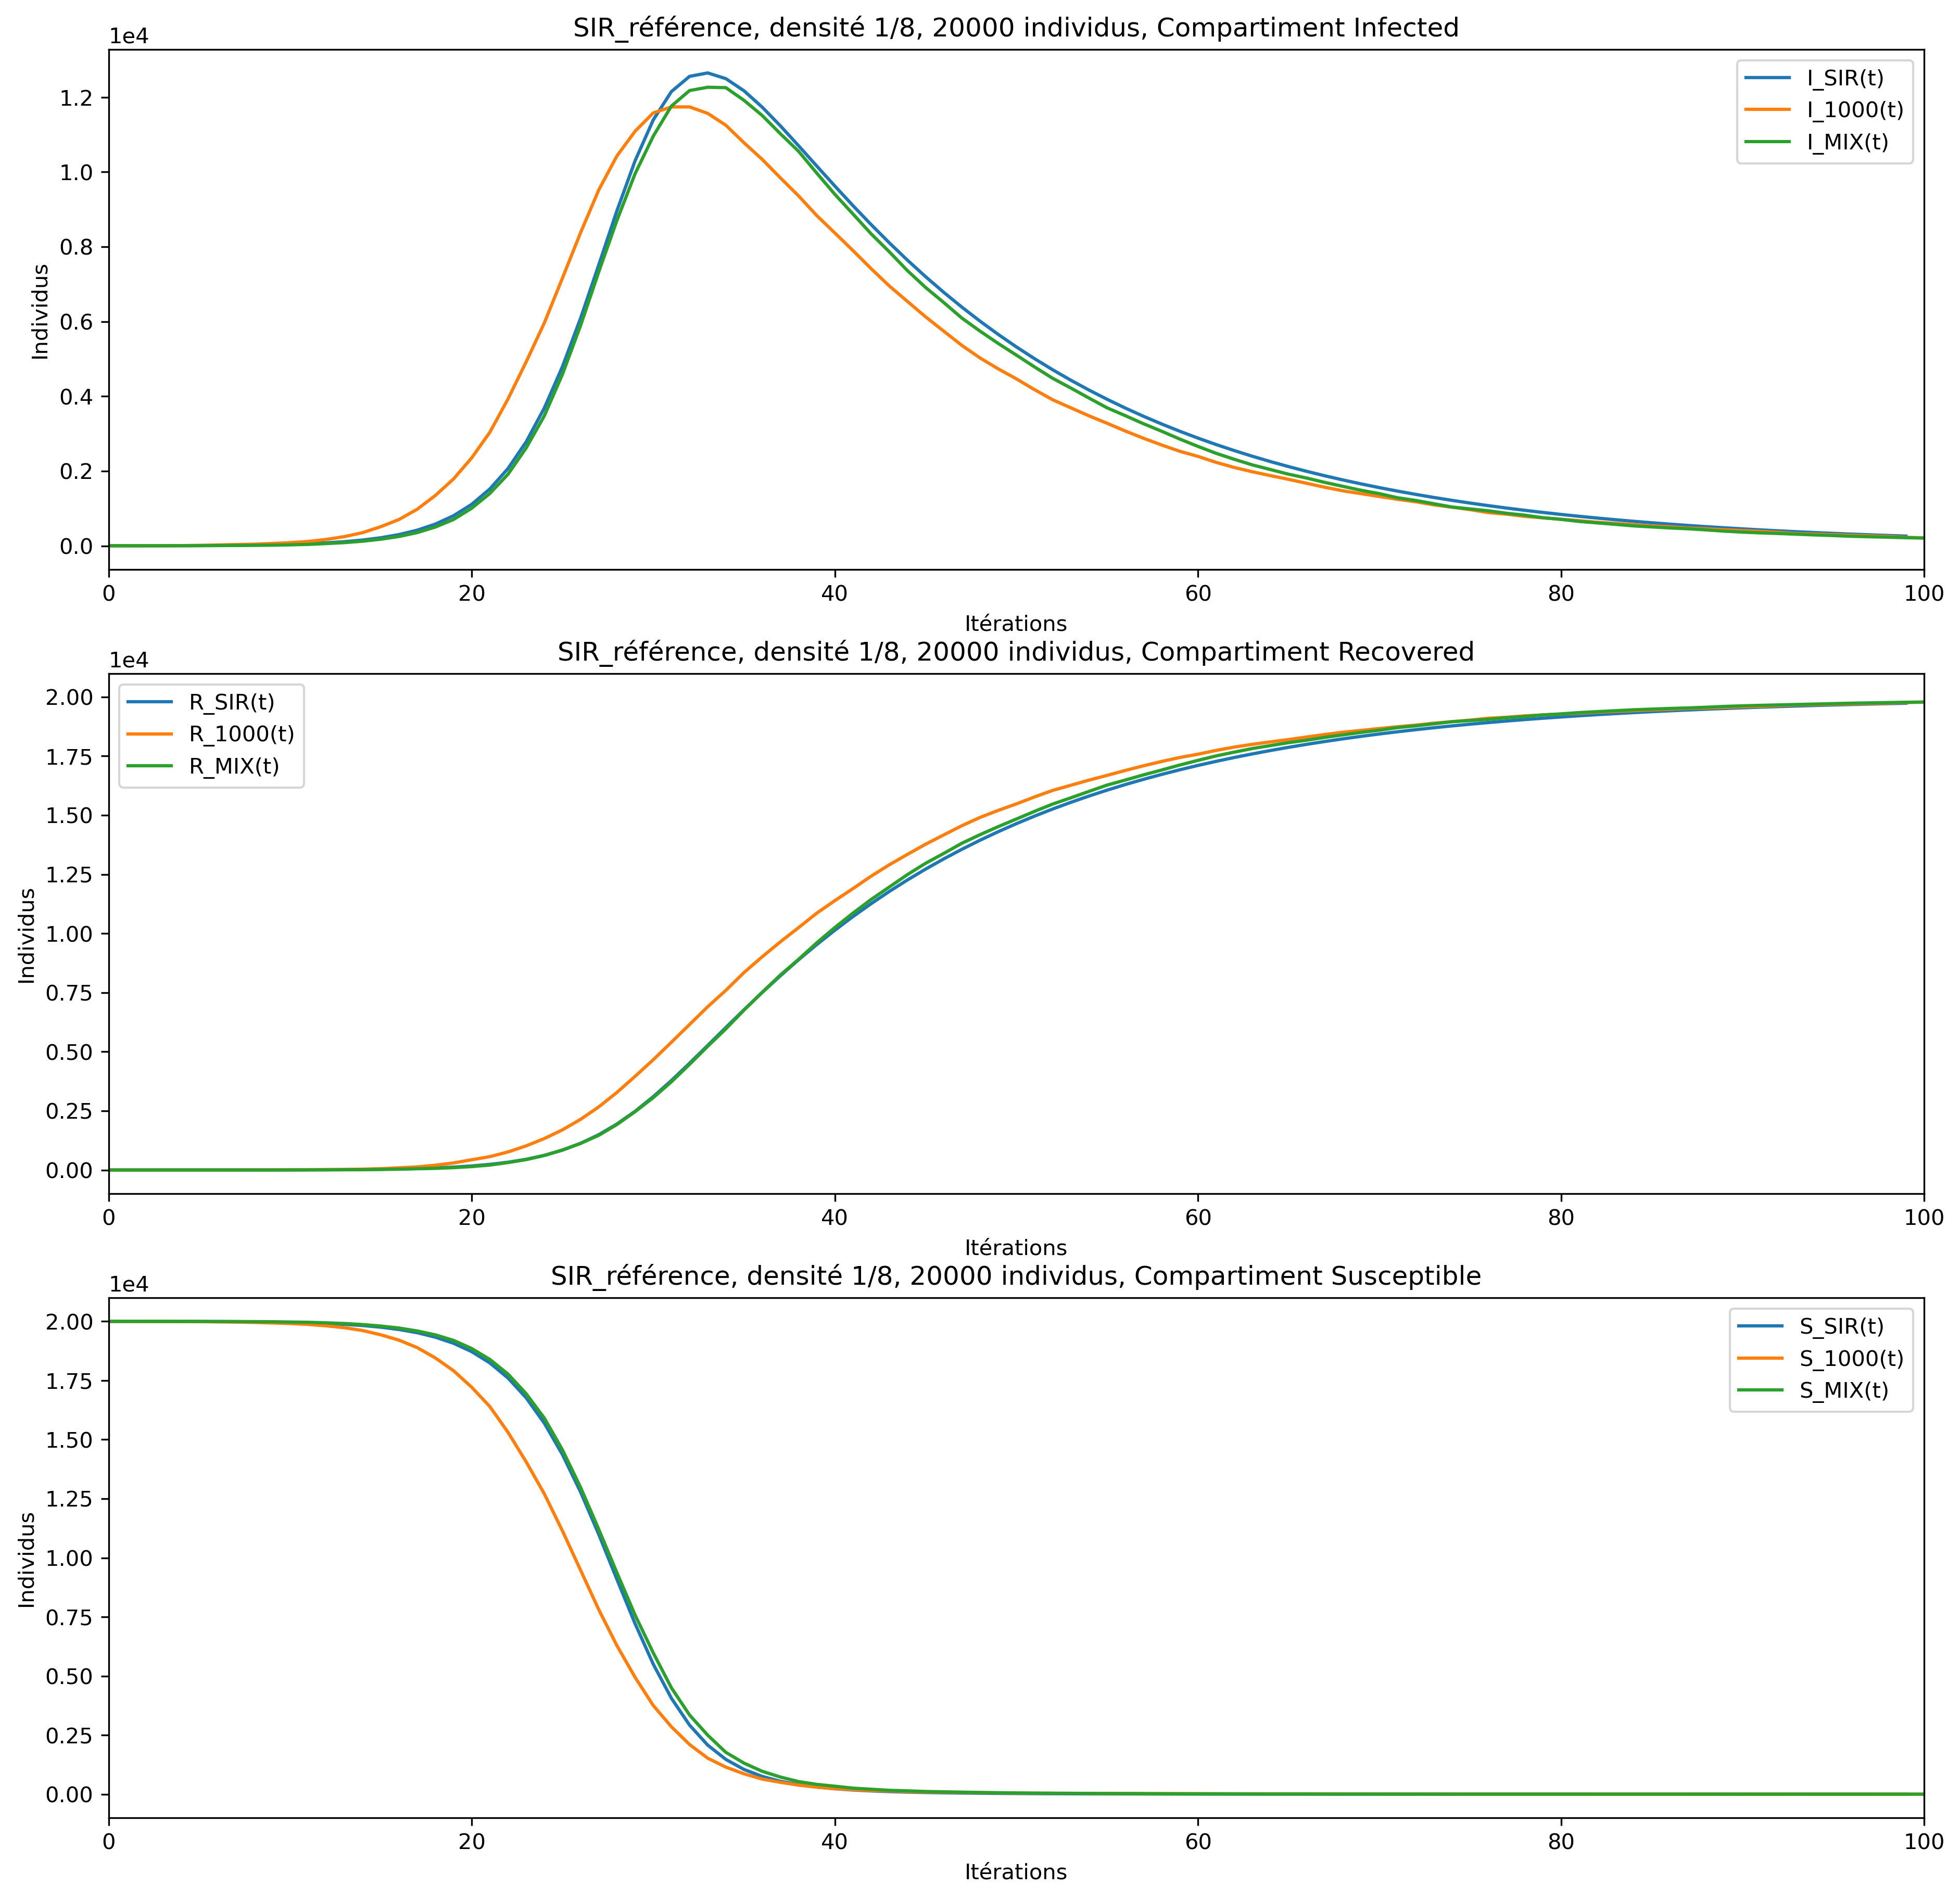
\includegraphics[width=.4\textwidth]{Images/SIR_ref_8_20.png}
	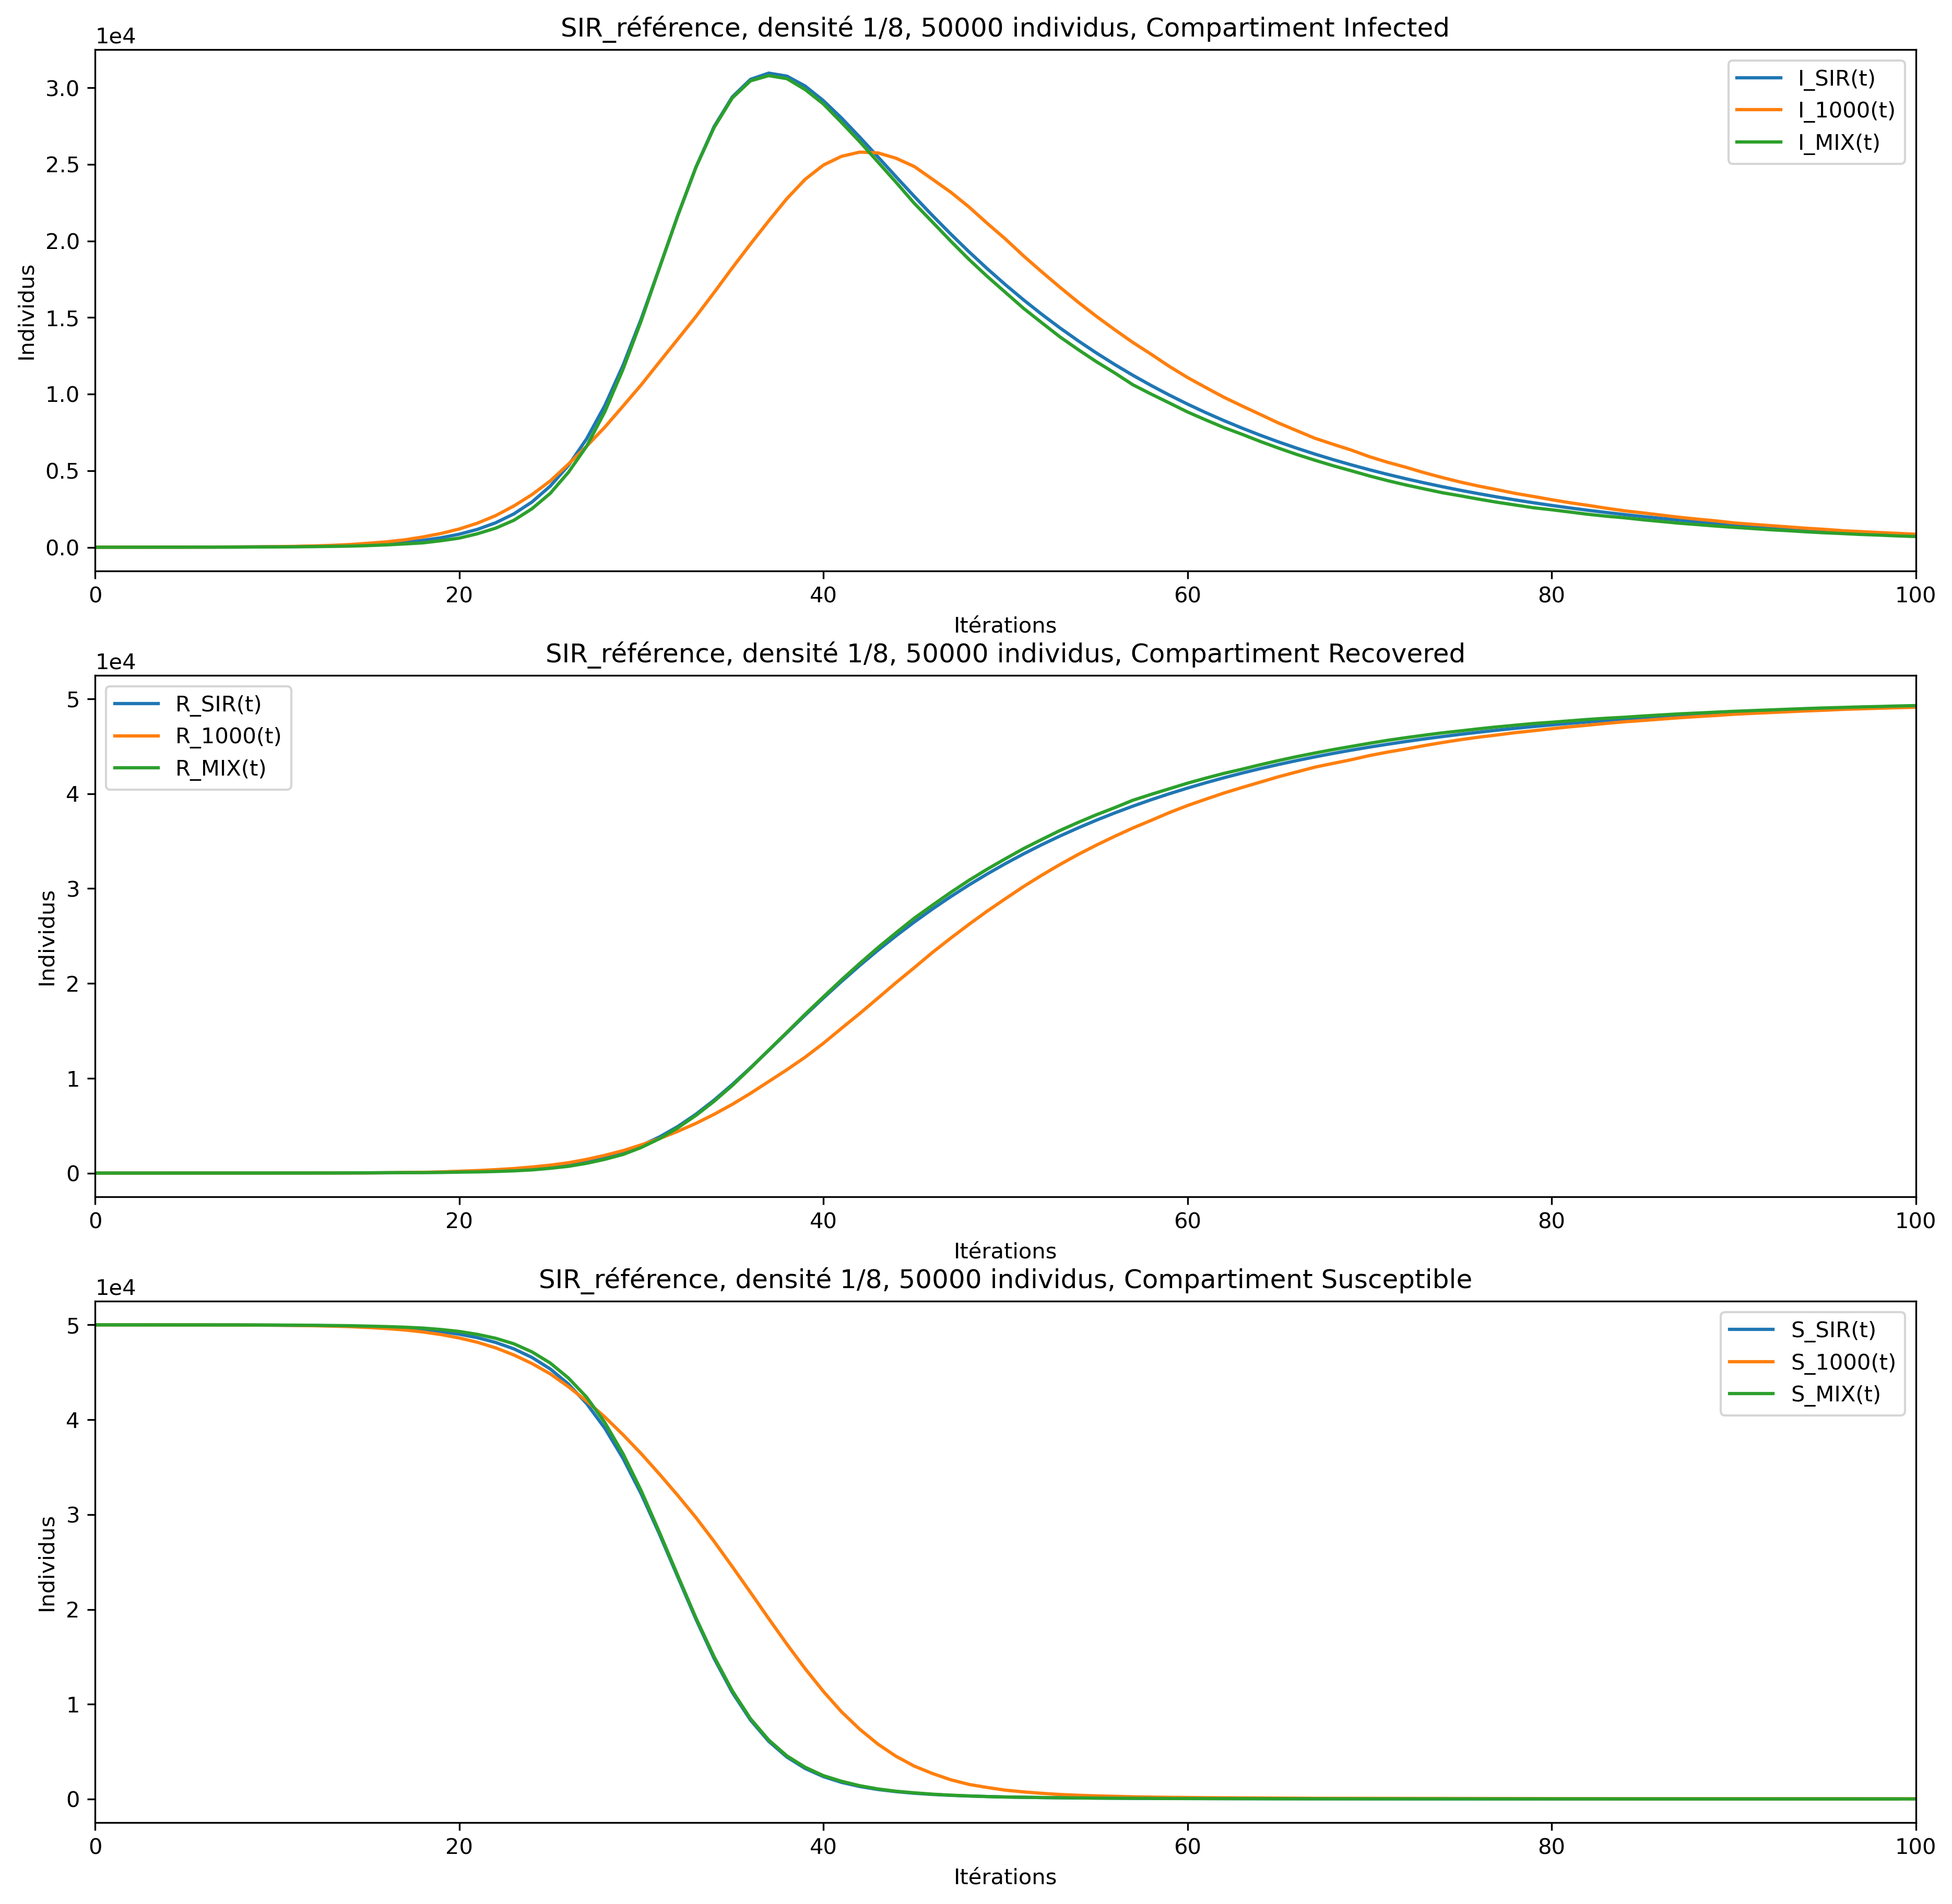
\includegraphics[width=.4\textwidth]{Images/SIR_ref_8_50.png}
	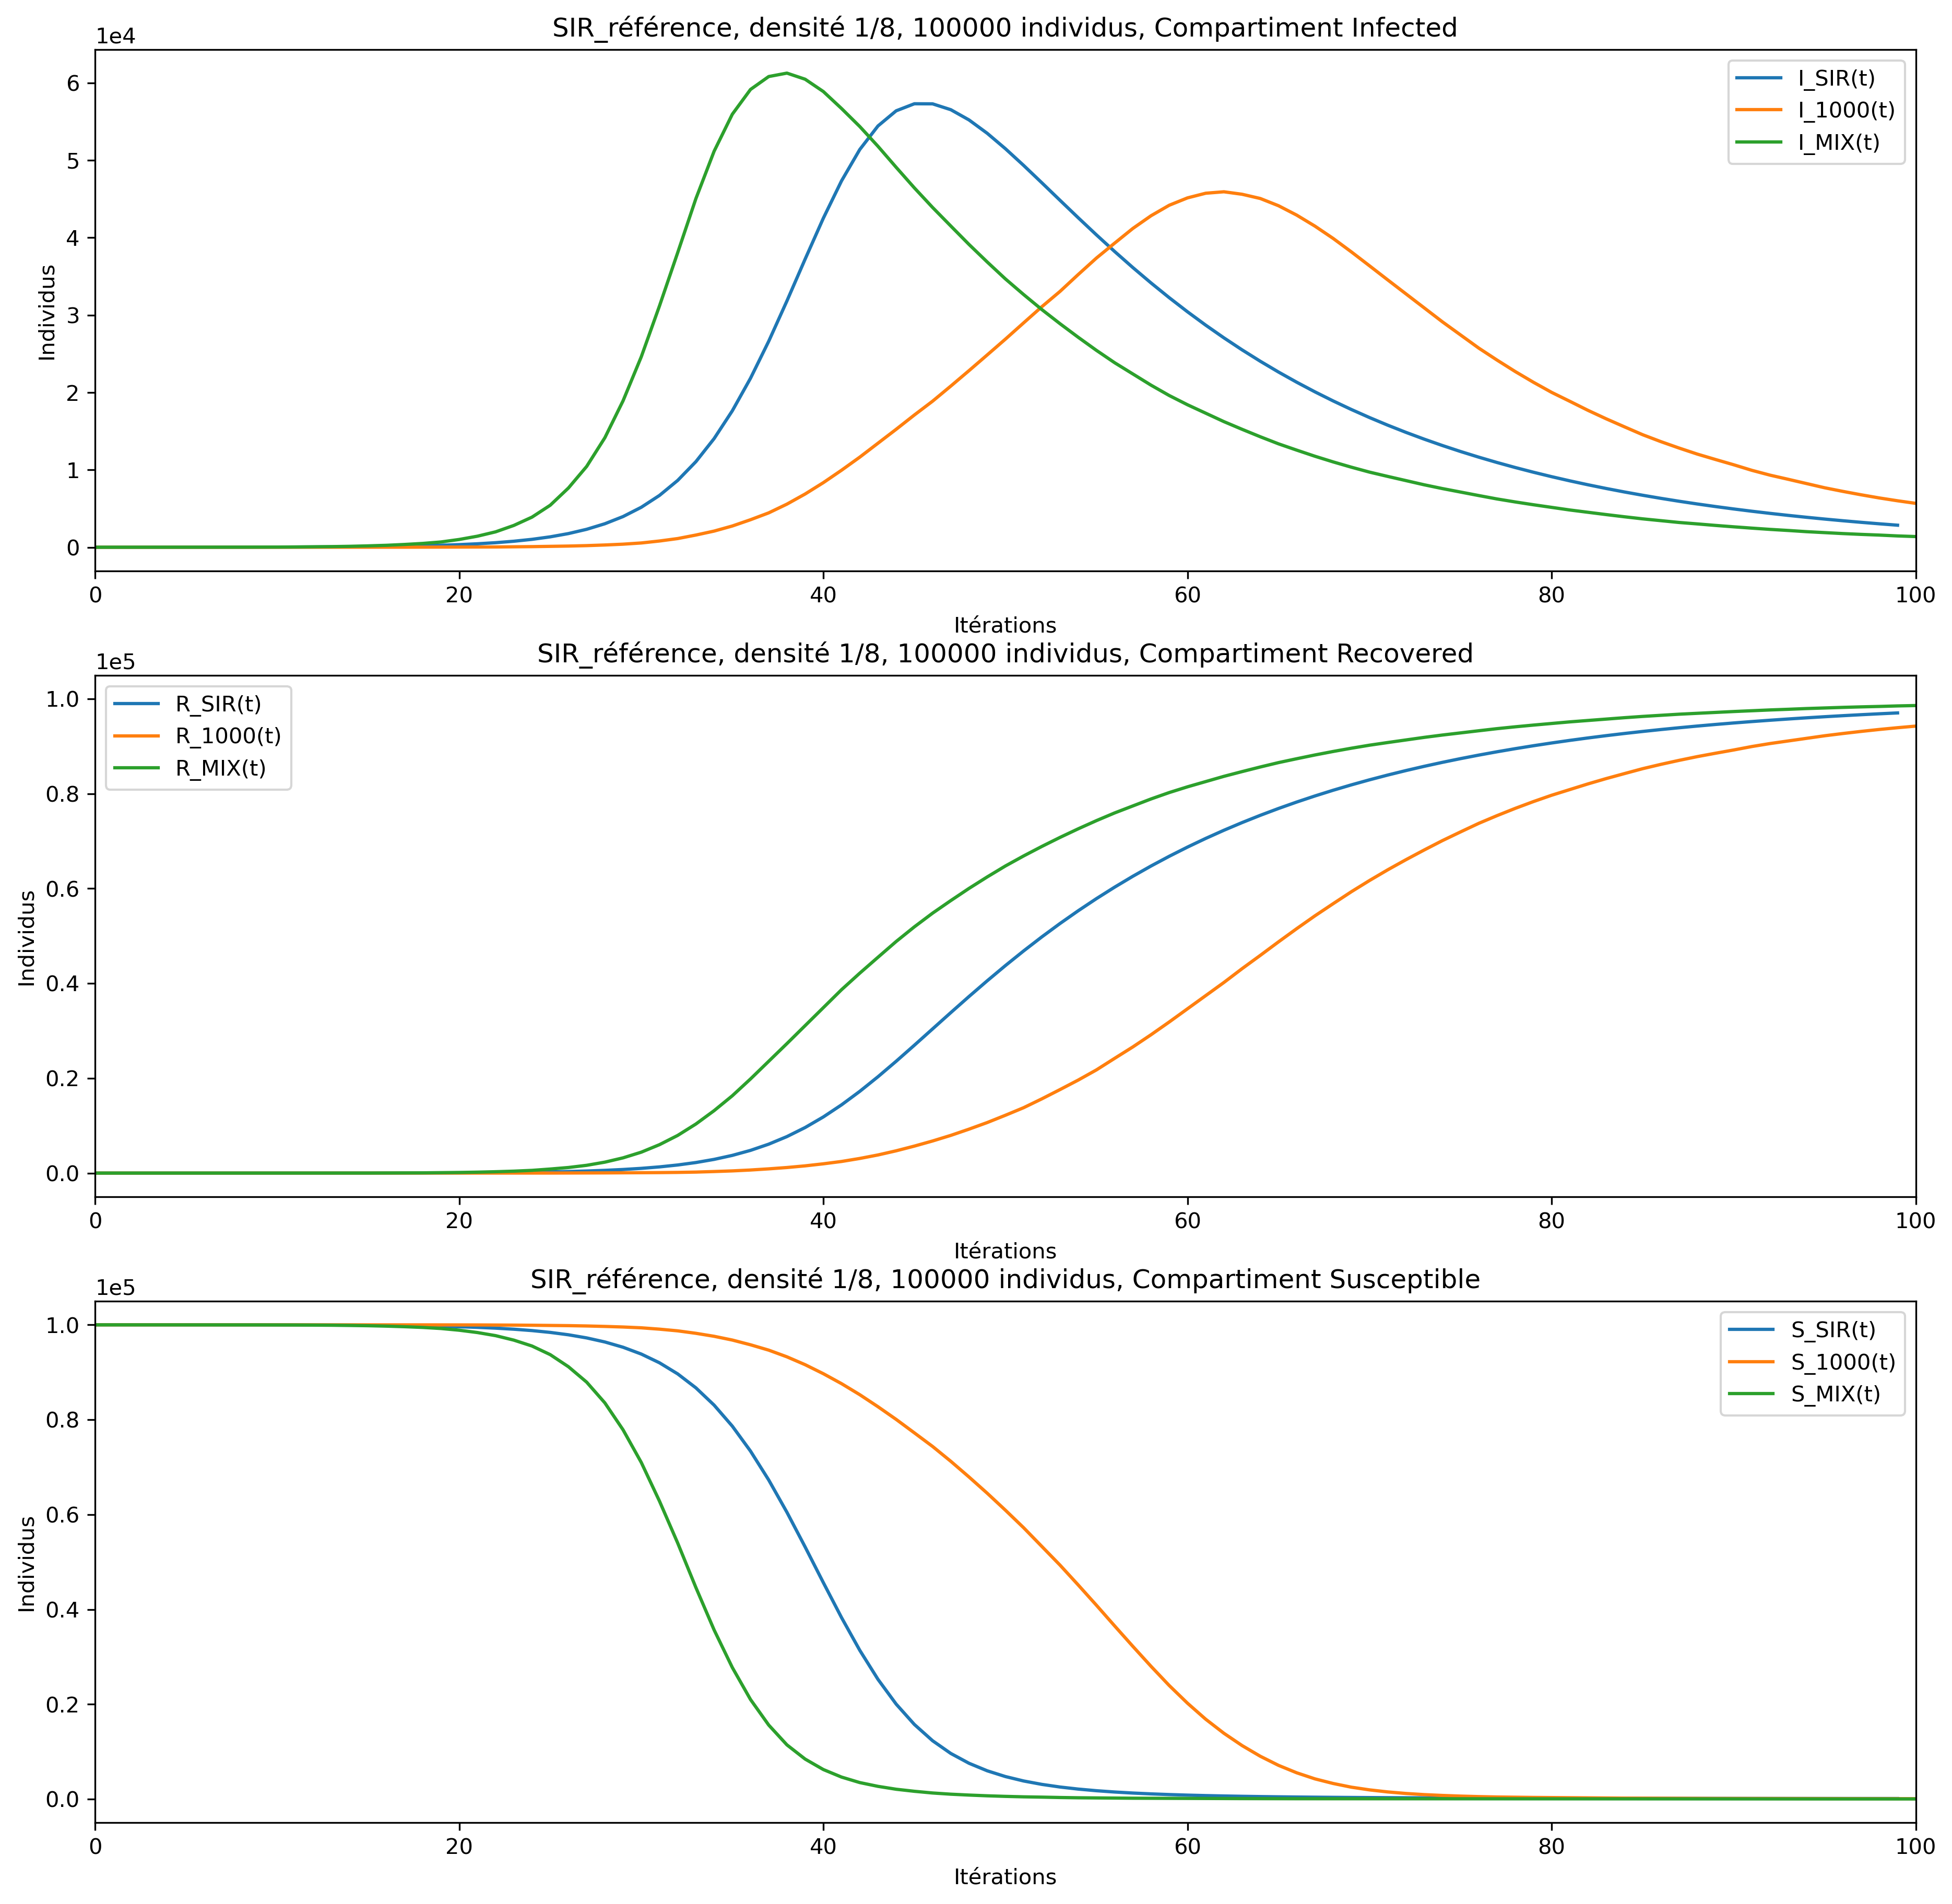
\includegraphics[width=.4\textwidth]{Images/SIR_ref_8_100.png}
	\caption{test}
\end{figure}

En plus de retrouver les mêmes comportements qu'observés précédemment, il y a un nouveau phénomène que nous pouvons observer ici. Ce phénomène est particulièrement présent dans les simulations à $5000$, $20000$ et $100000$ individus. Nous remarquons que la croissance des courbes pour les simulations de mélange parfait sont plus rapides que le modèle mathématique SIR. Ce comportement est dû au fait que nos simulations peuvent nécessiter d'un temps de latence avant l'émergence d'un événement. Alors que au contraire le modèle SIR n'est pas victime de cette latence.\\

Par conséquent, pour joindre le modèle SIR aux simulations il faut prendre en compte le temps de latence et l'ajouter au modèle SI artificiellement. Ce temps de latence est particulièrement présent sur les systèmes peu denses car dans ces configurations les pandémies peuvent prendre du temps à apparaitre. Ce phénomène est étudié dans un autre chapitre.

\newpage

\begin{figure}[h]
	\centering
	\captionsetup{justification=centering}
	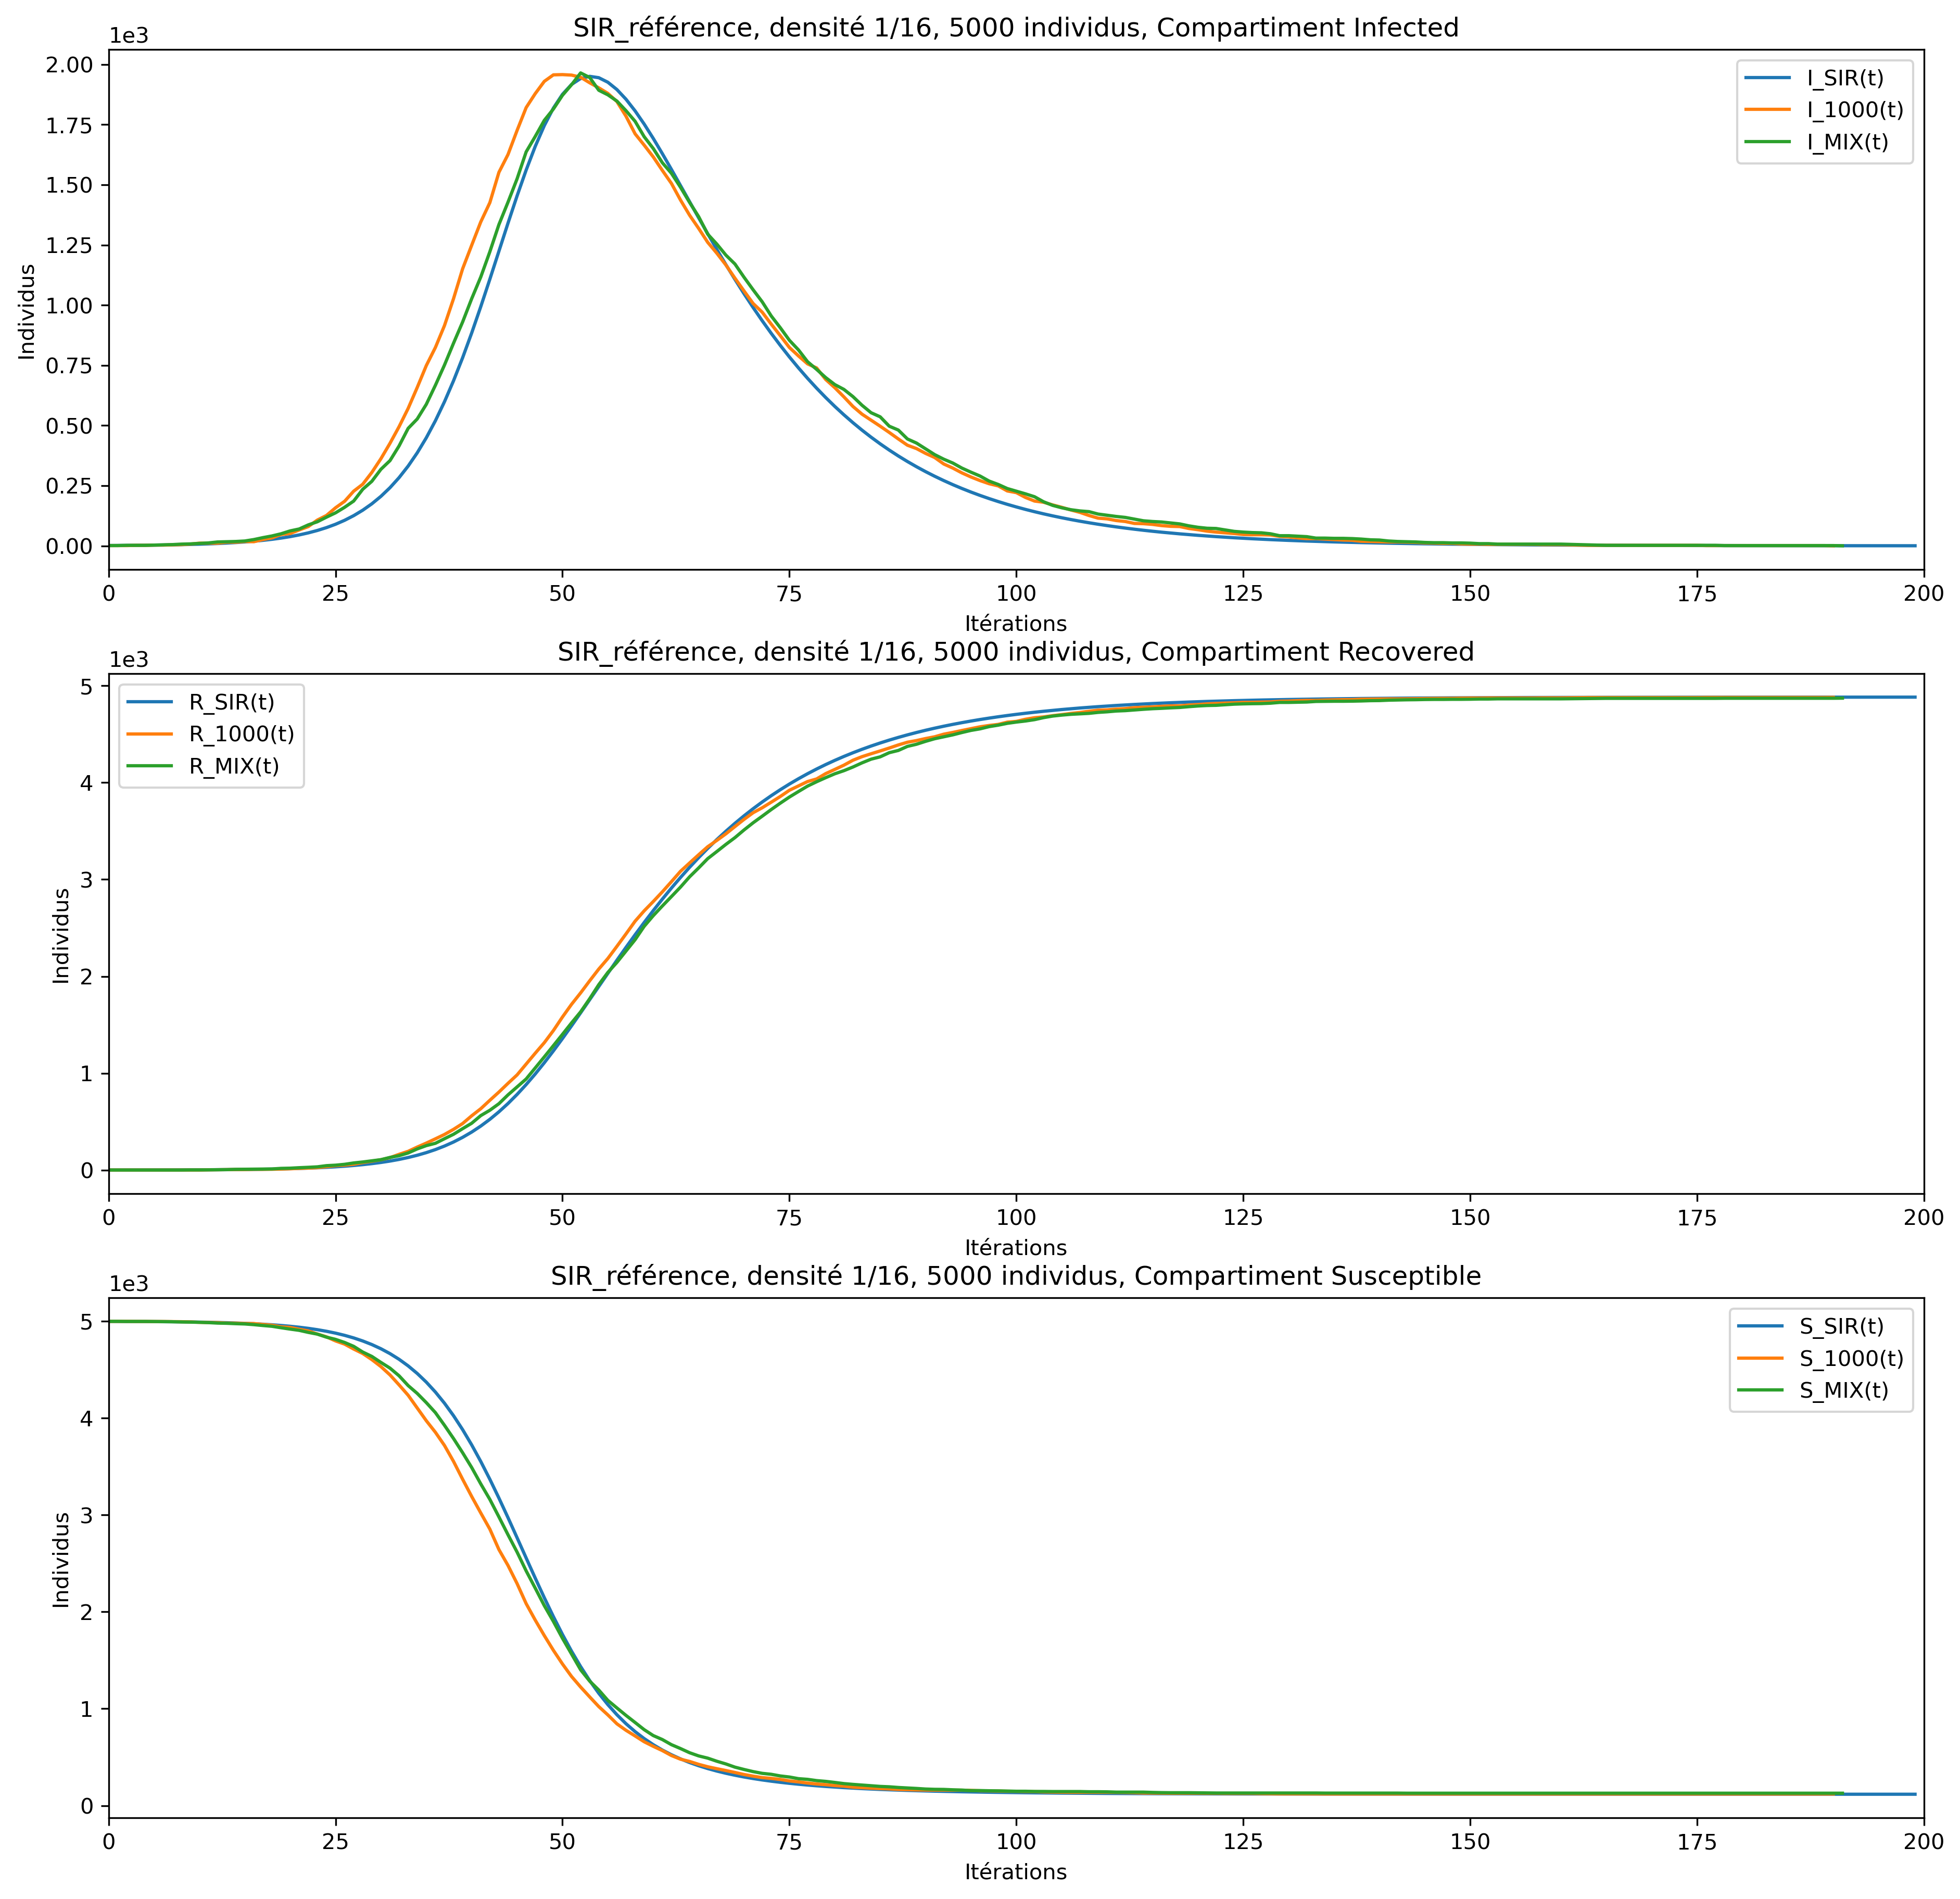
\includegraphics[width=.4\textwidth]{Images/SIR_ref_16_5.png}
	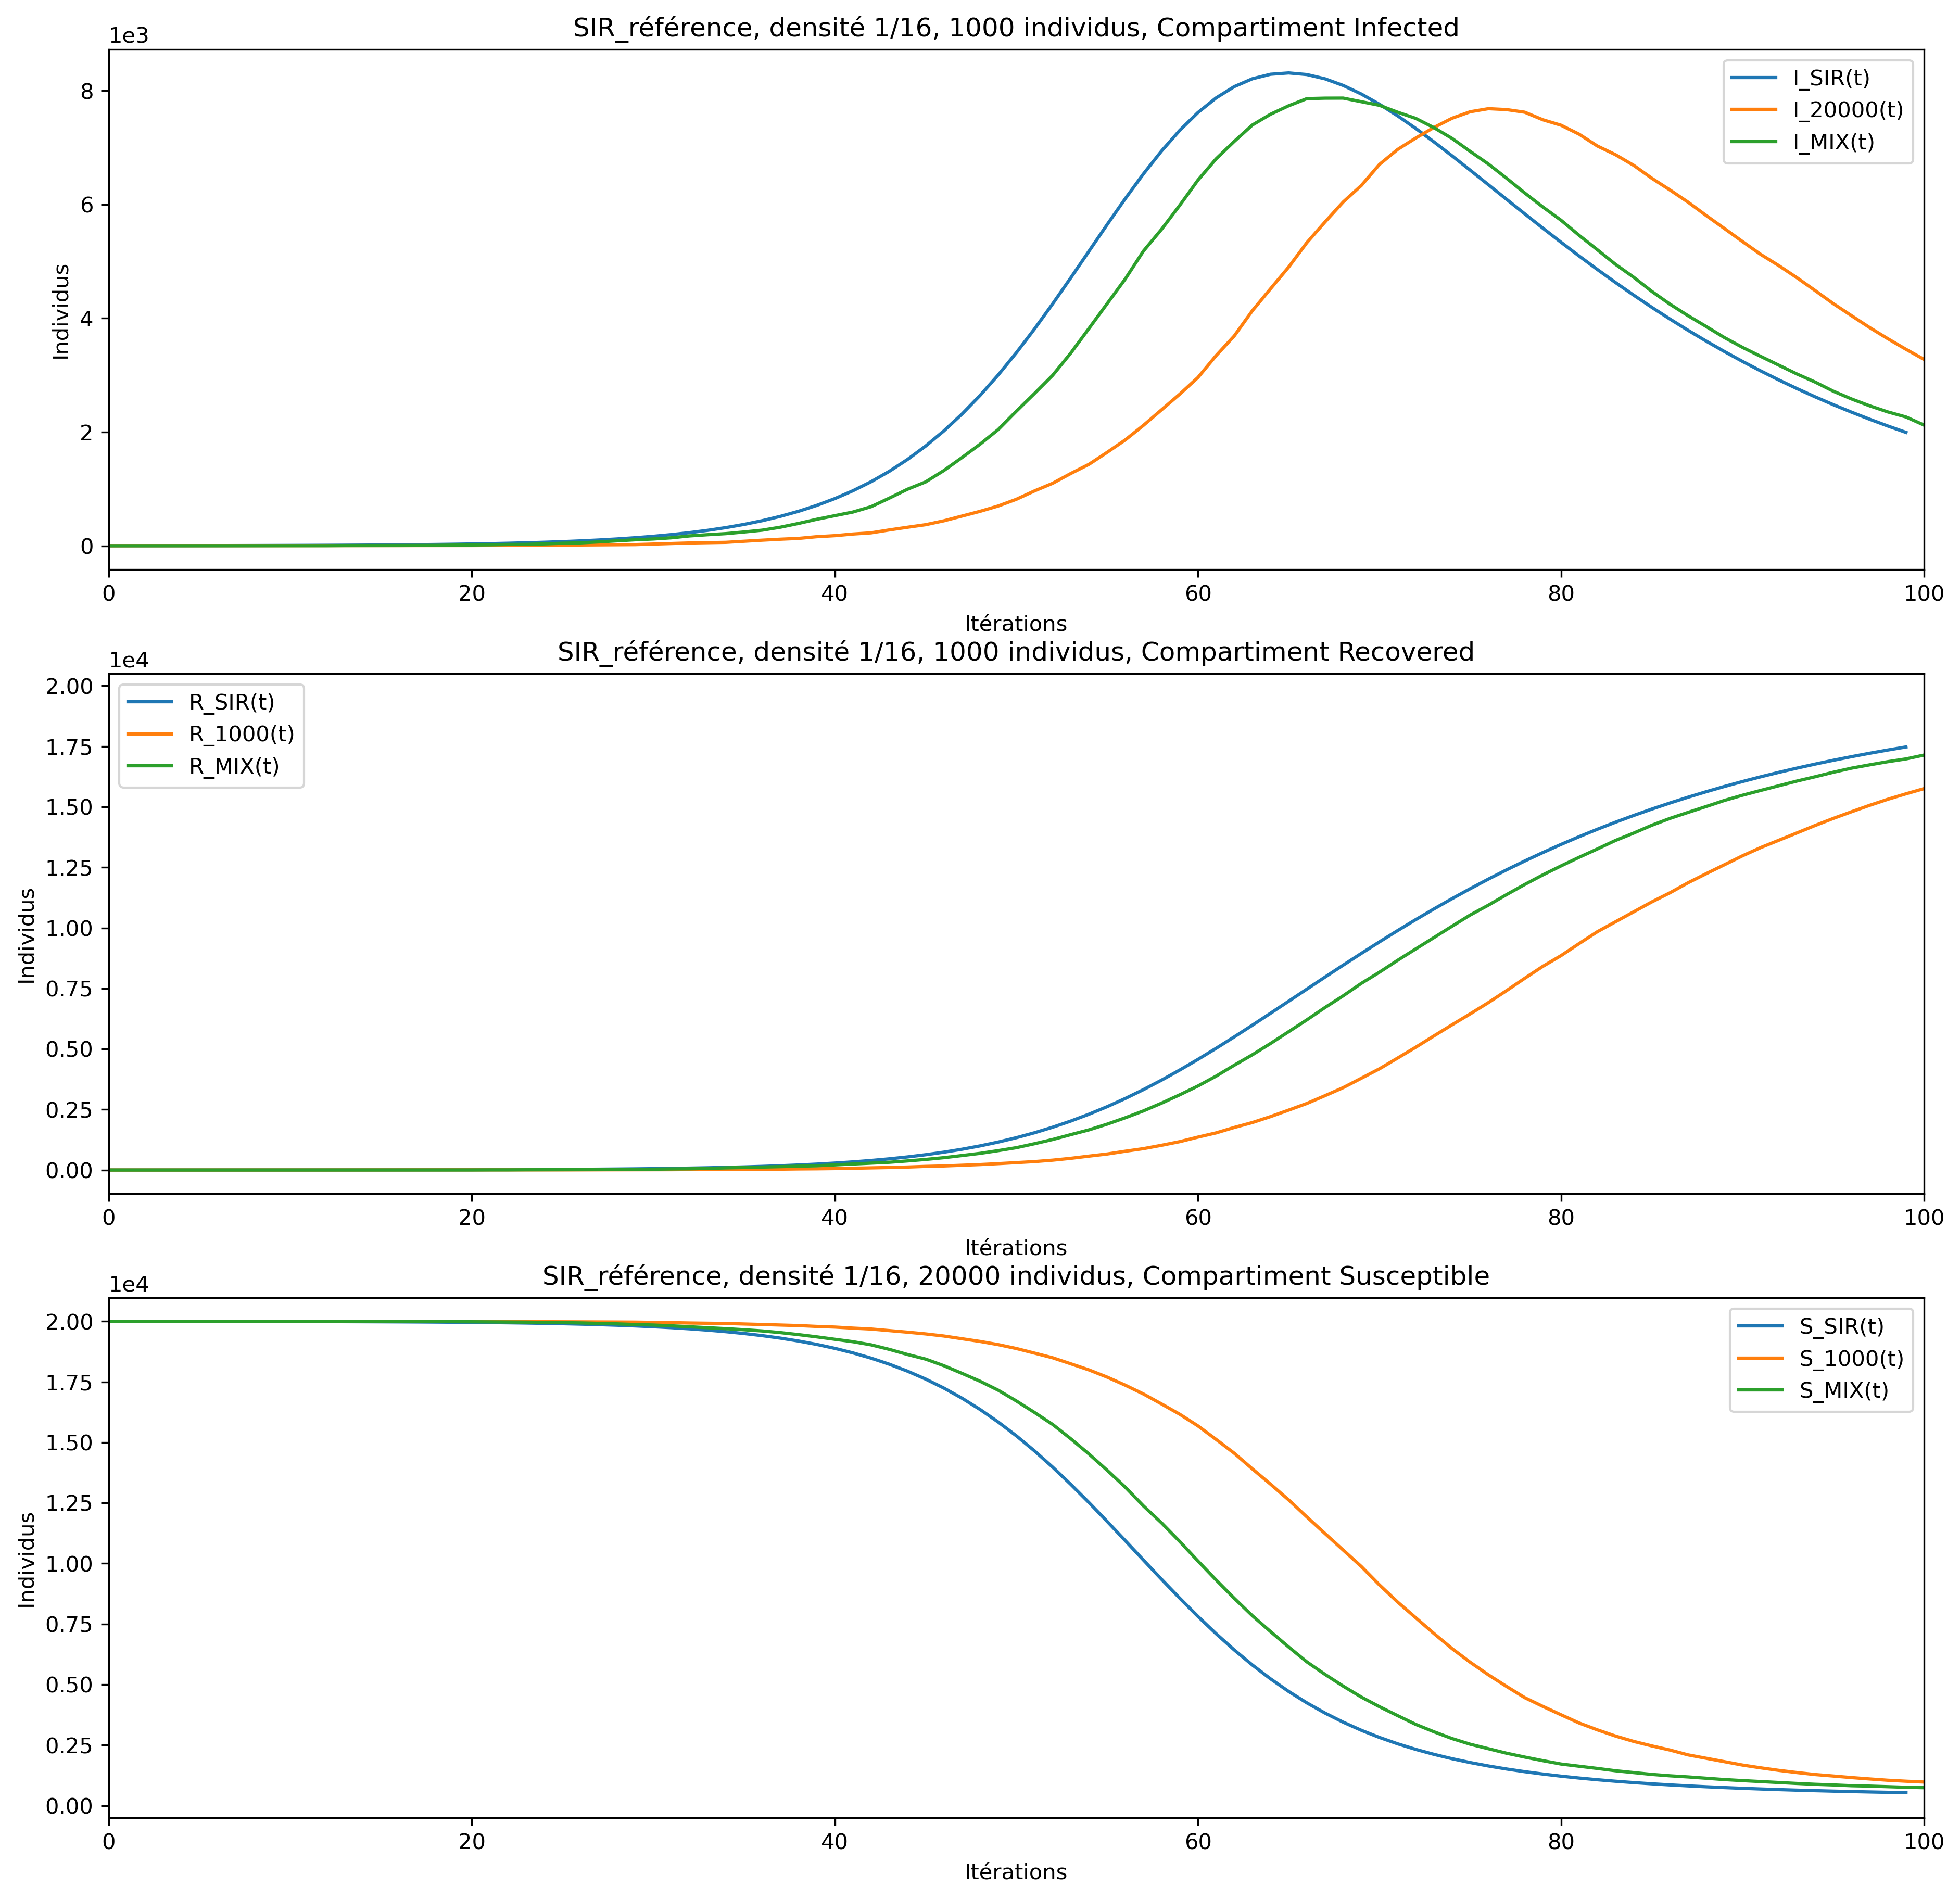
\includegraphics[width=.4\textwidth]{Images/SIR_ref_16_20.png}
	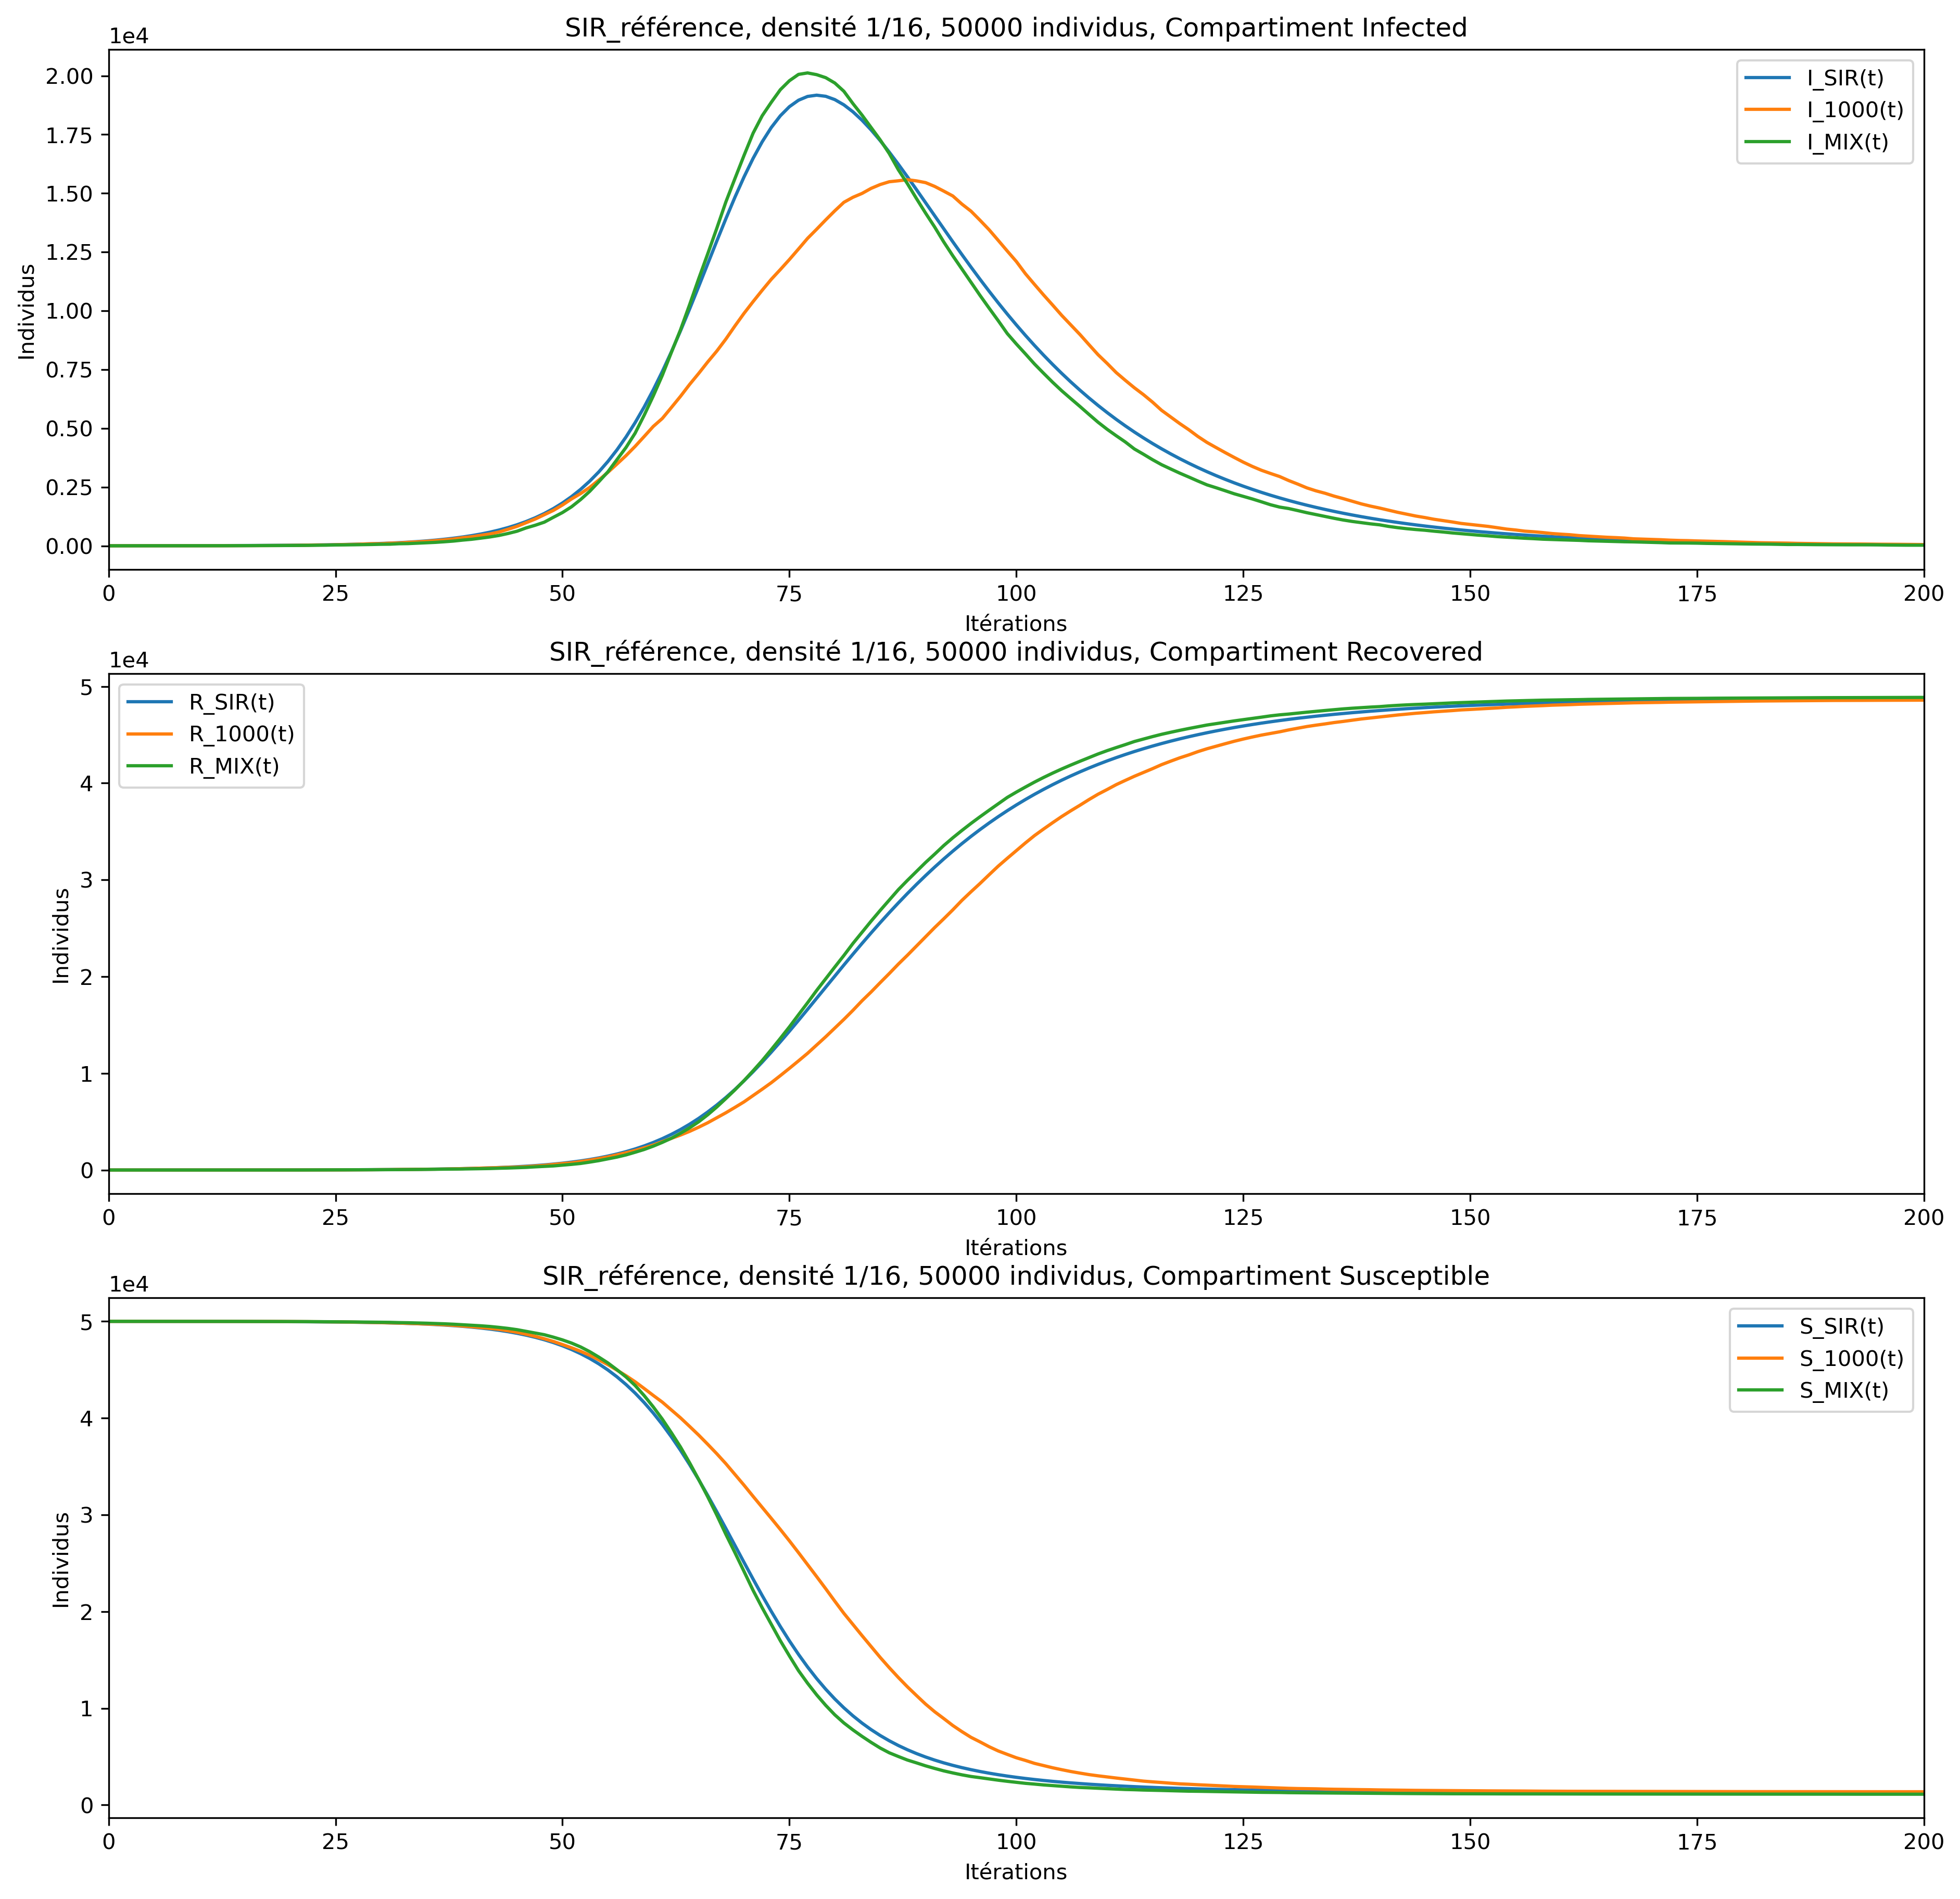
\includegraphics[width=.4\textwidth]{Images/SIR_ref_16_50.png}
	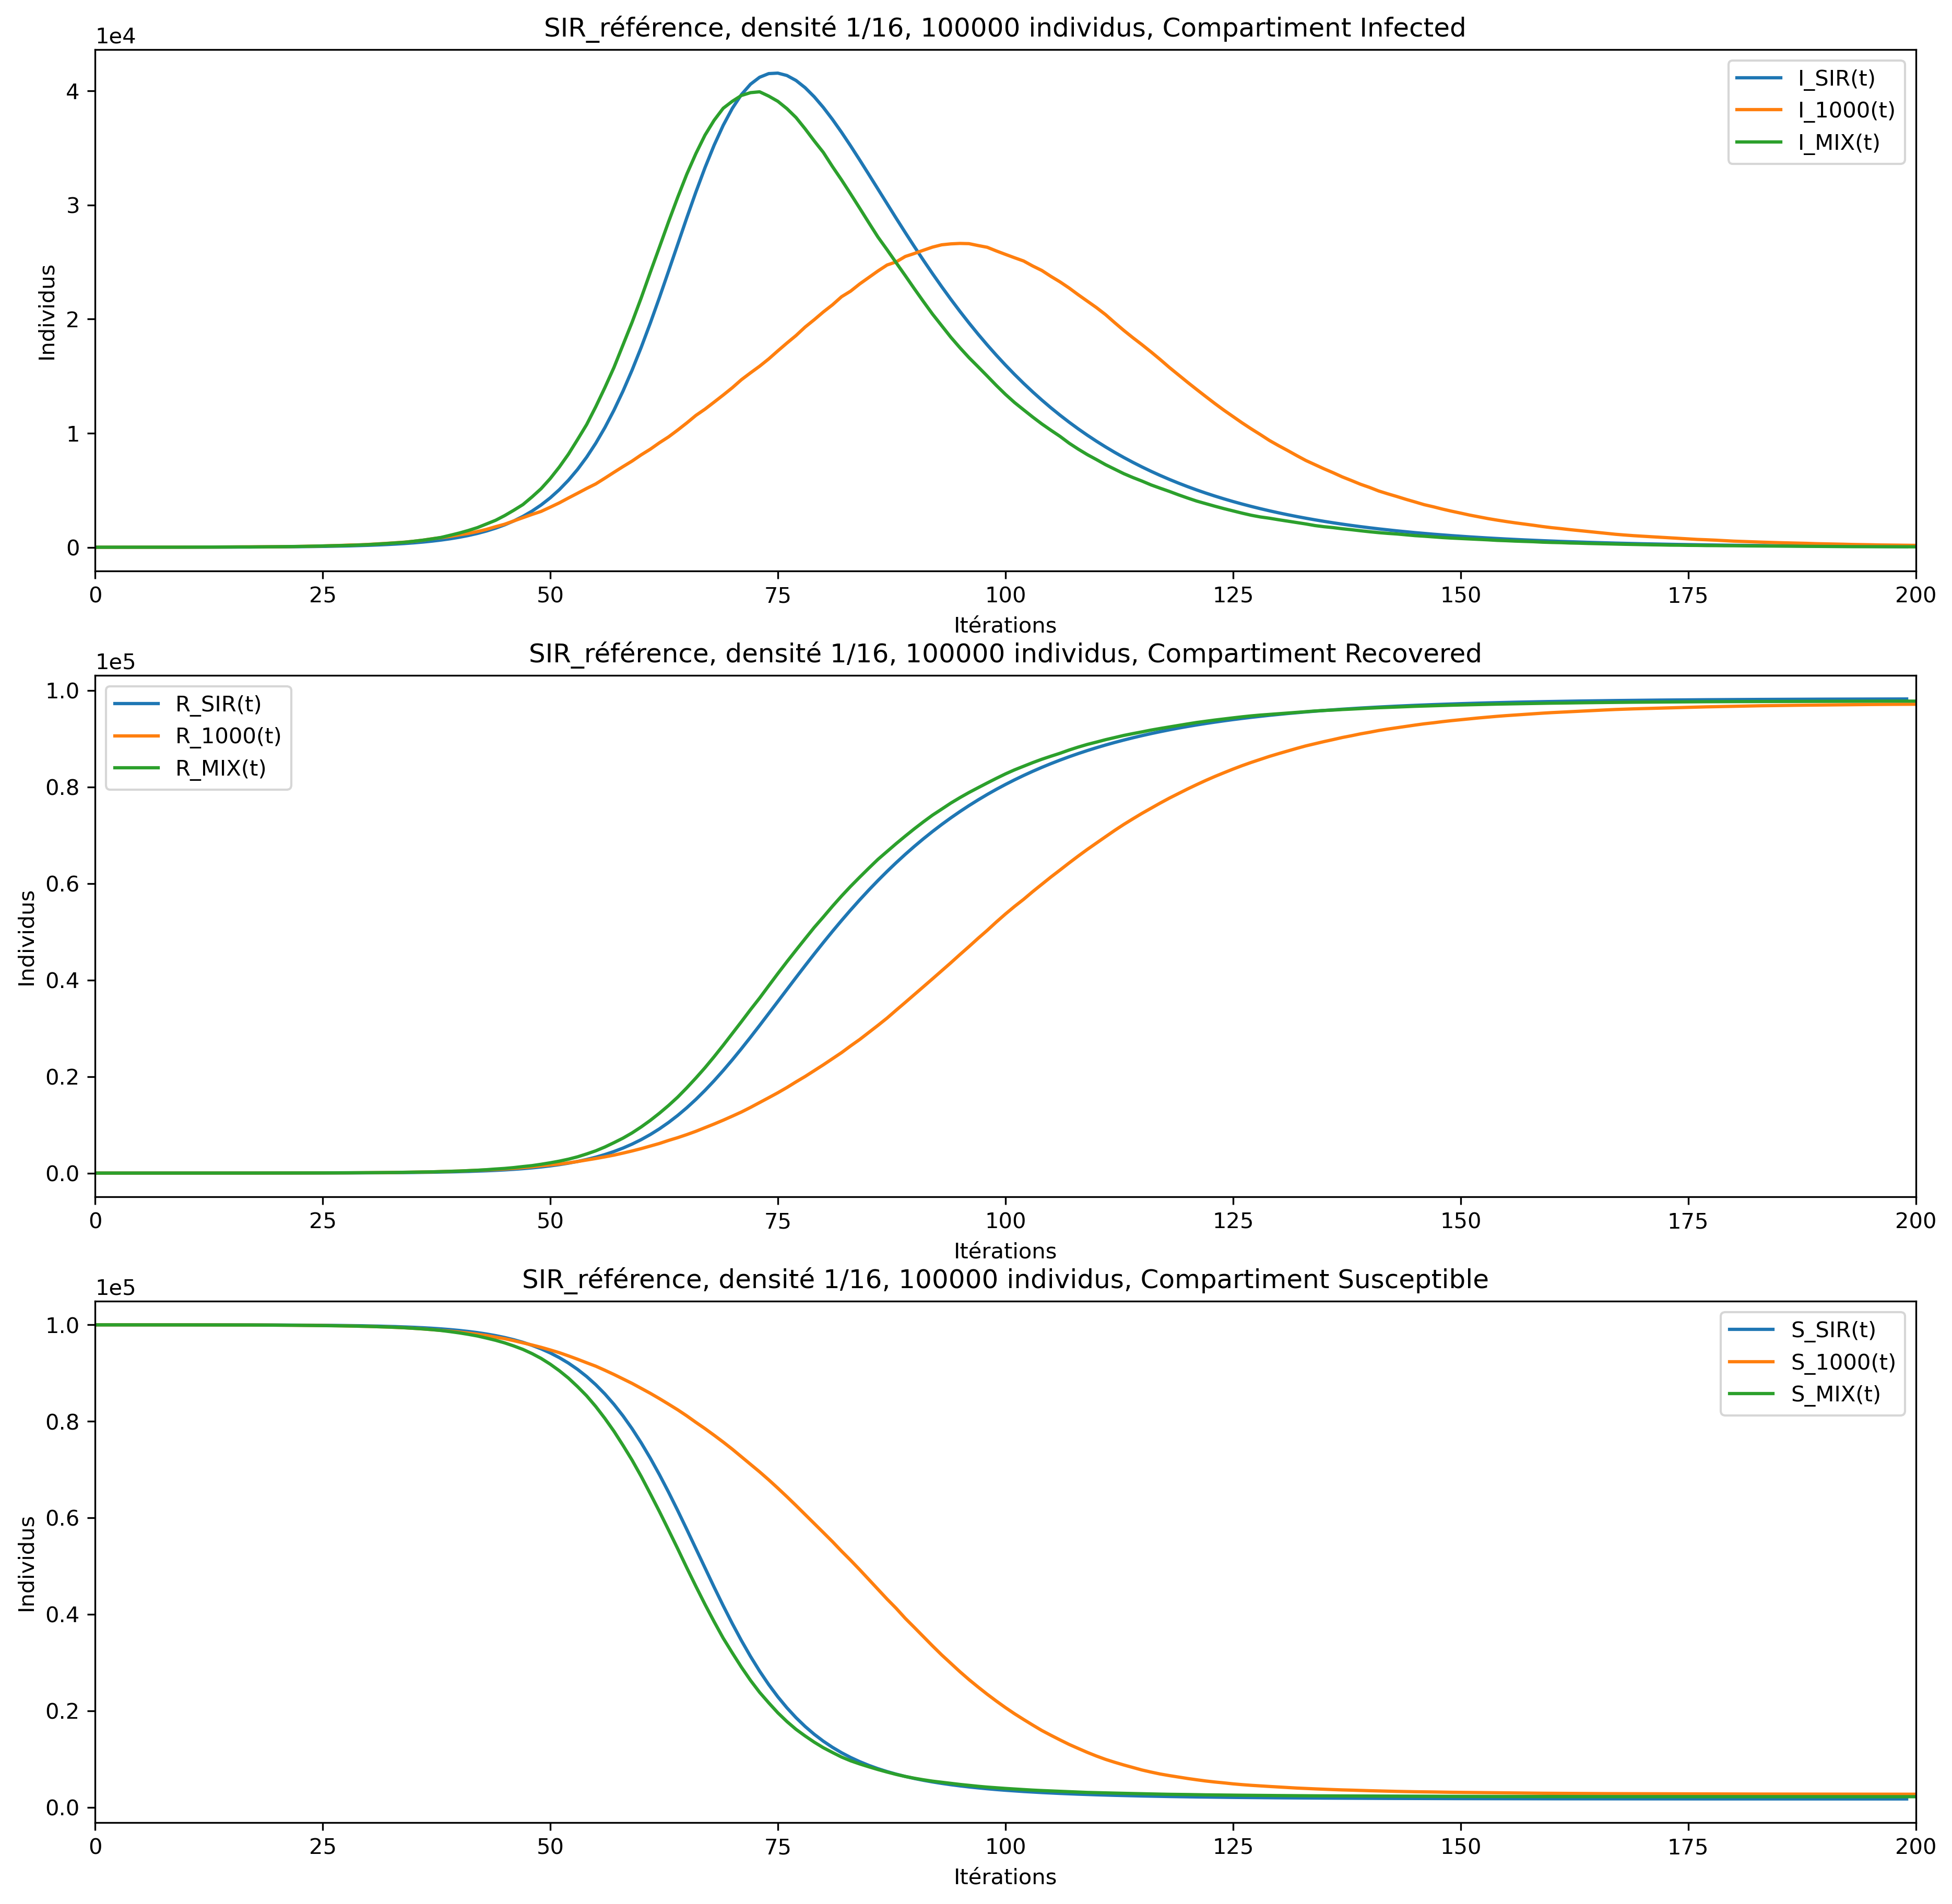
\includegraphics[width=.4\textwidth]{Images/SIR_ref_16_100.png}
	\caption{test}
\end{figure}

Tout comme pour le modèle SI, les simulations aux $1000$ mouvements sont ralenties par les systèmes de grande taille car le mouvement des individus est réduit par rapport à la taille du système. C'est la raison pour laquelle les courbes au $1000$ mouvements sont retardées.\\

Malgré des observations déjà analysées, nous obsevons des oscillations sur la simulation à $5000$ indiviuds. Ce phénomène n'était pas présent sur les simulations SI et ceci à cause de l'absense du compartiment $Recovered$. Deux raisons explique ce comportement, le premier est que le mécanisme d'immunisation transfert des individus du compartiment $I$ au $R$ et donc abaisse la courbe. Le second est dû à la densité du système qui est très faible, par conséquent il y a peu de contactes qui s'effectuent ce qui crée des oscillations. Ces oscillations sont aussi présentes sur des sytèmes plus denses mais pas perceptibles car moyennée par un grand nombre d'événements.

\section{Analyses}

\subsection{Mean Absolute Error}

Le mean absolute error permet de quantifier les différences entre les simulations et le modèle mathématique SIR. Les calculs suivants ont été effectués sur les simulations au mélnage parfait. Contrairement au modèle SI, le modèle SIR contient trois courbes différentes par conséquent chacune de ces courbes a sont propre MAE. Le tableau ci-dessous donne la moyenne de ces trois résultats et ceci pour toutes les simulations SIR.

\begin{table}[H]
	\centering
	\captionsetup{justification=centering}
	\caption[Mean Aboslute Error Normalized : SI]{Mean Aboslute Error Normalized : modèle SIR, mélange parfait \label{tab:grid}}
	\begin{tabular}{@{\extracolsep{\fill} } c|| c| c| c| c|}
	 & 5000 & 20000 & 50000 & 100000\\ 
	\midrule
	\midrule
	1/2 & $4.3\mathrm{e}{-3}$ & $2.1\mathrm{e}{-3}$ & $2.7\mathrm{e}{-3}$ & $2.5\mathrm{e}{-3}$\\
	\midrule
	1/4 & $3.8\mathrm{e}{-3}$ & $3.0\mathrm{e}{-3}$ & $2.1\mathrm{e}{-3}$ & $2.6\mathrm{e}{-3}$\\
	\midrule
	1/8 & $9.6\mathrm{e}{-3}$ & $2.8\mathrm{e}{-3}$ & $1.9\mathrm{e}{-3}$ & $2.3\mathrm{e}{-3}$\\
	\midrule
	1/16 & $8.5\mathrm{e}{-3}$ & $3.2\mathrm{e}{-3}$ & $6.2\mathrm{e}{-3}$ & $7.2\mathrm{e}{-3}$\\
	\bottomrule
	\end{tabular}
	\end{table}

Les tésultats pour le modèle SIR sont généralement moins précis que pour le modèle SI. Certains résultats sont intéressant par exemple les courbes de densité $\frac{1}{8}$ avec $5000$ individus. L'erreur sur cette courbe est élevée car la simulation souffre de latence, par conséquent le déclanchement de l'événement se fait tardivement. C'est également la raison pour laquelle la simulation au $1000$ mouvement évolue plus rapidement que la simulation au mélange parfait.\\

En densité $frac{1}{16}$ d'avantage d'erreurs apparaissent. Premièrement, une plus grande erreur de la simulation à $5000$ individus et due aux oscillations causées par le peu d'événements du système, donc les systèmes peu denses ont une plus grande erreur. Deuxièmement les simulations à faible densité prennent du temps déclancher un événement, ce qui engendre un temps de latence. Ce temps de latence est innexistant dans le modèle SIR, par conséquent notre modèle ne se comporte plus exactement comme un modèle mathématique SIR.

\subsection{Positions des individus}

Cette section a pour but de visualiser l'impacte de la densité des systèmes sur les déplacements des individus et donc sur la qualité du mélange. Les figures suivantes montrent les positions géographiques de tous les individus à une certaine itération. En vert sont affichés les individus sains et en rouge les individus contaminés.\\

L'image ci-dessous montre les positions des individus pour une simulation au mélange parfait à l'itération $20$. Le mode de mélange parfait redistribue tous les individus dans l'espace à chaque itération, par conséquent les individus contaminés sont parfaitement répartis dans l'espace.

\begin{figure}[h]
	\centering
	\captionsetup{justification=centering}
	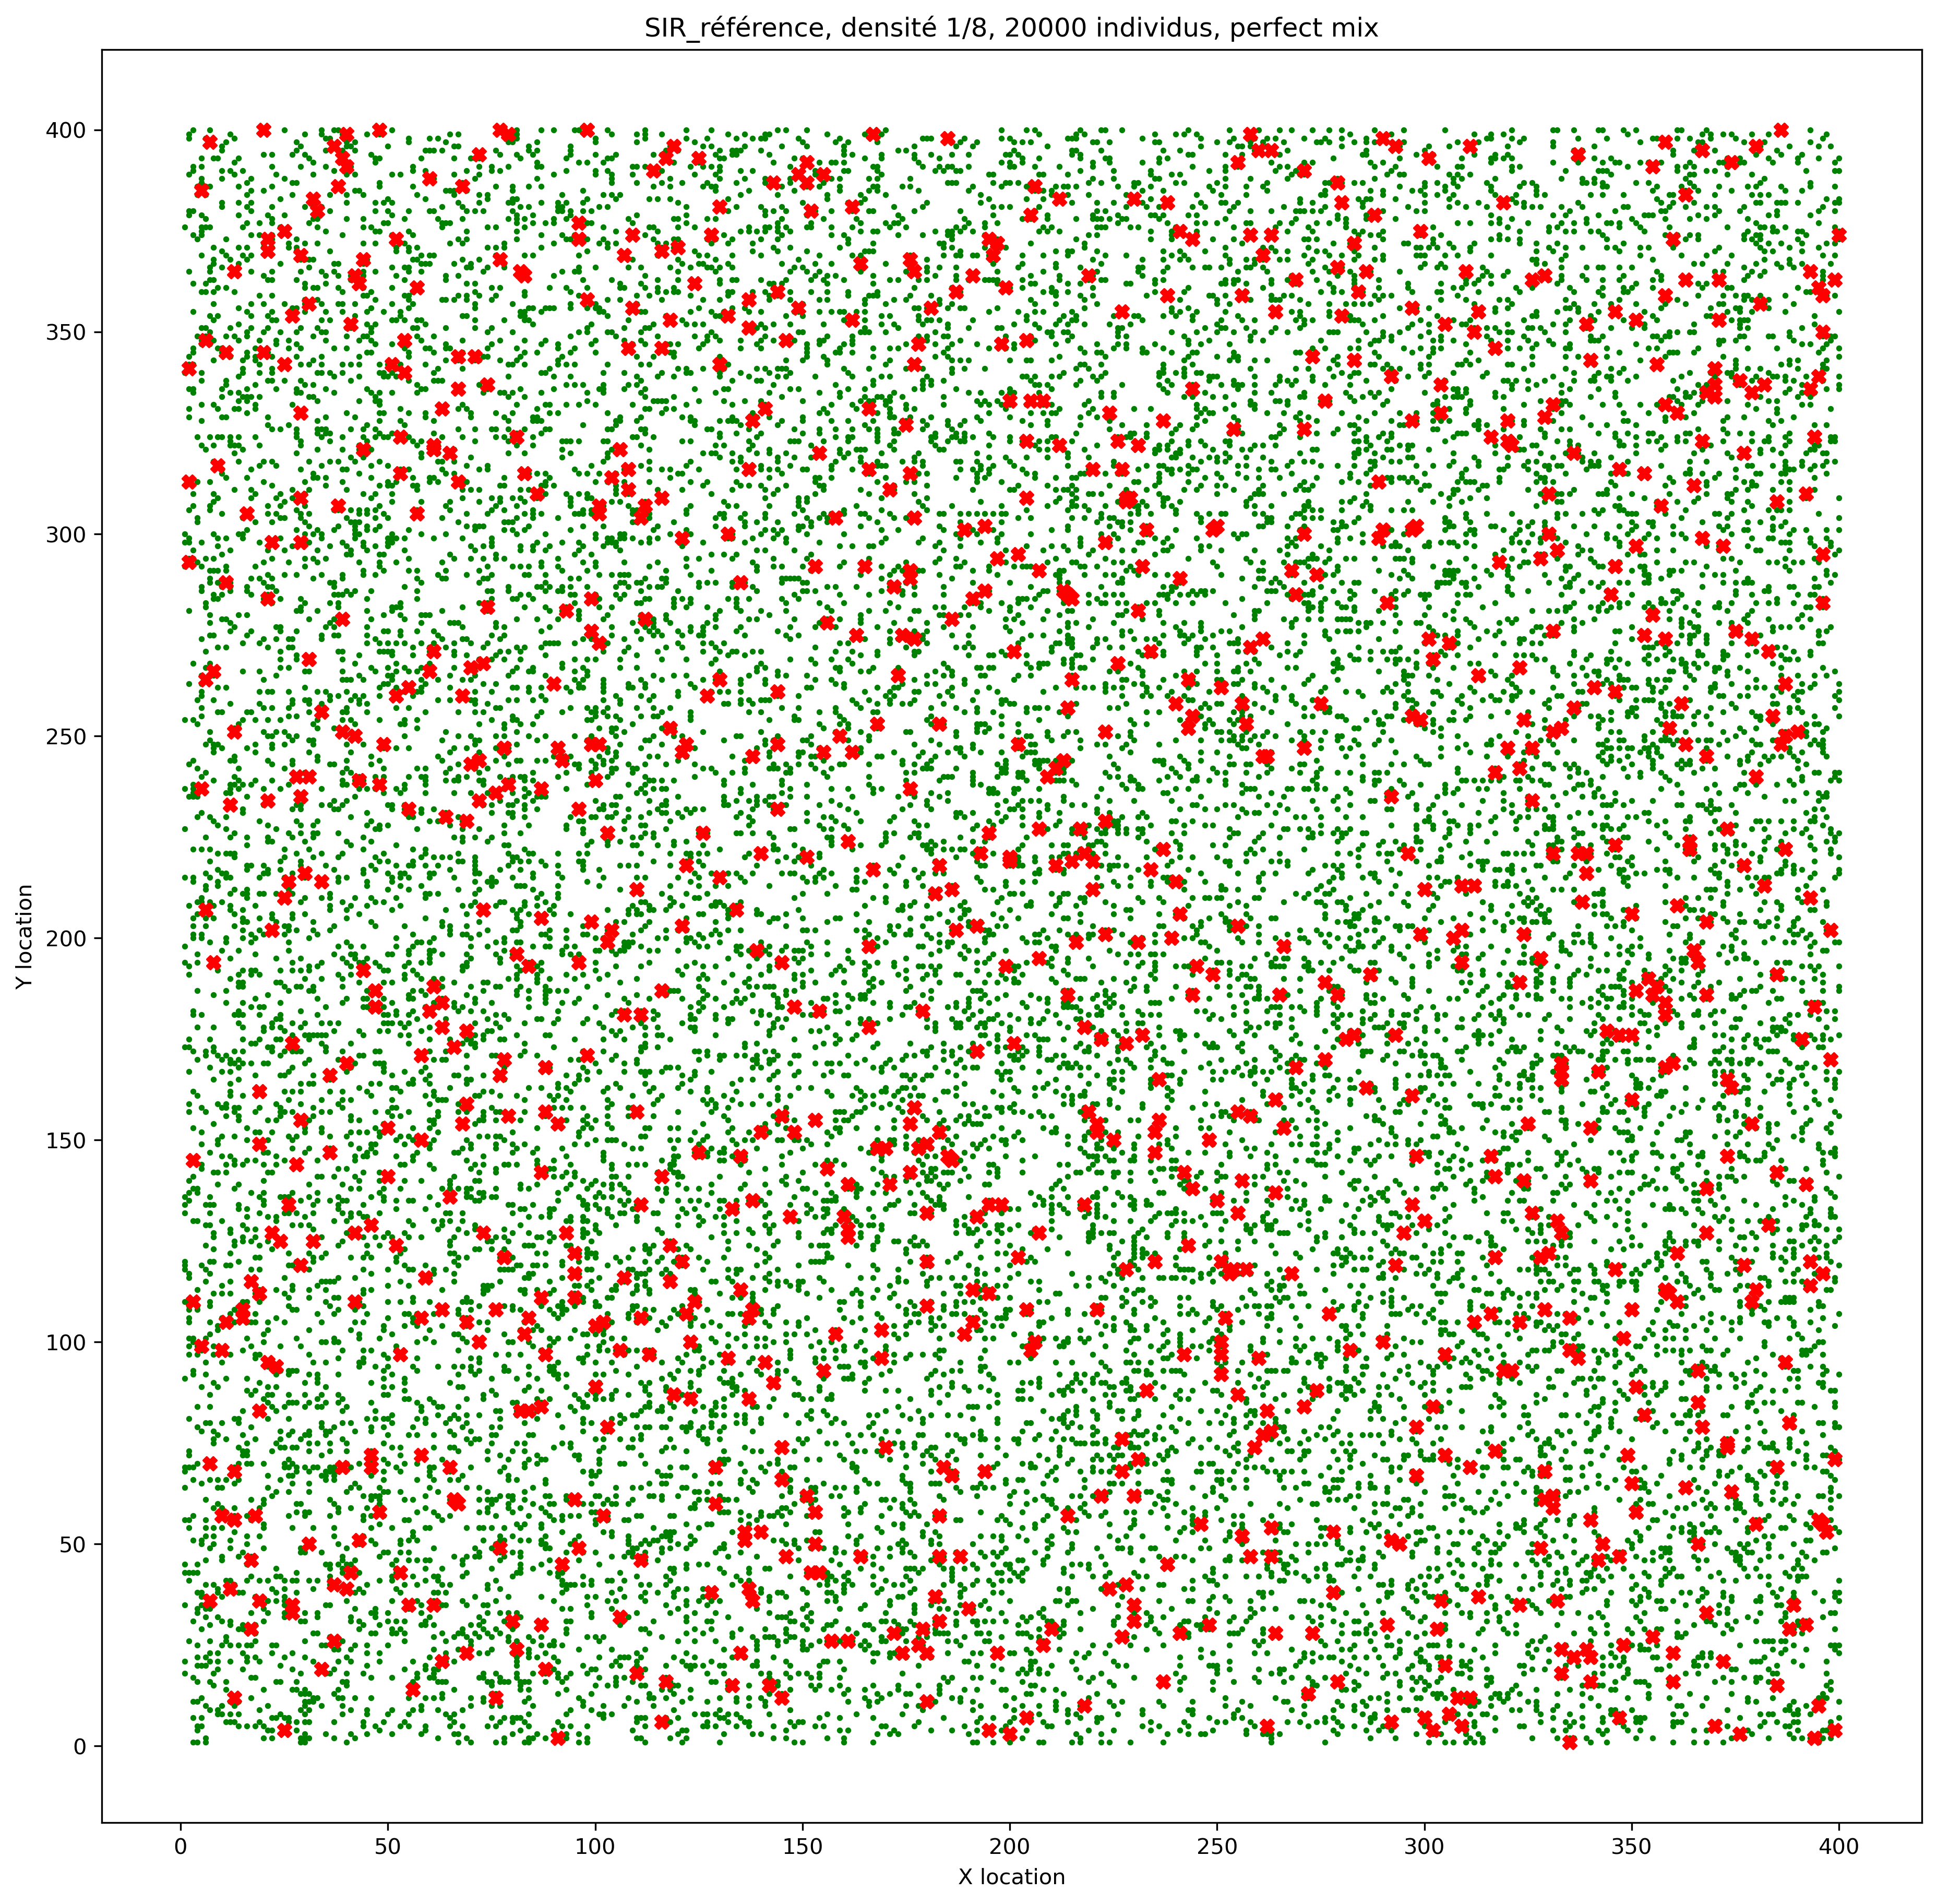
\includegraphics[width=.7\textwidth]{Images/SIR_position_8_20_perfect_mix.png}
	\caption{test}
\end{figure}

Sur les figures qui suivent, nous effectuons la même mesure mais cette fois-ci sur des simulations aux $1000$ mouvements. L'idée est de pouvoir observer la qualité du mélange de population en fonction de la densité du système.

\newpage

\begin{figure}[h]
	\centering
	\captionsetup{justification=centering}
	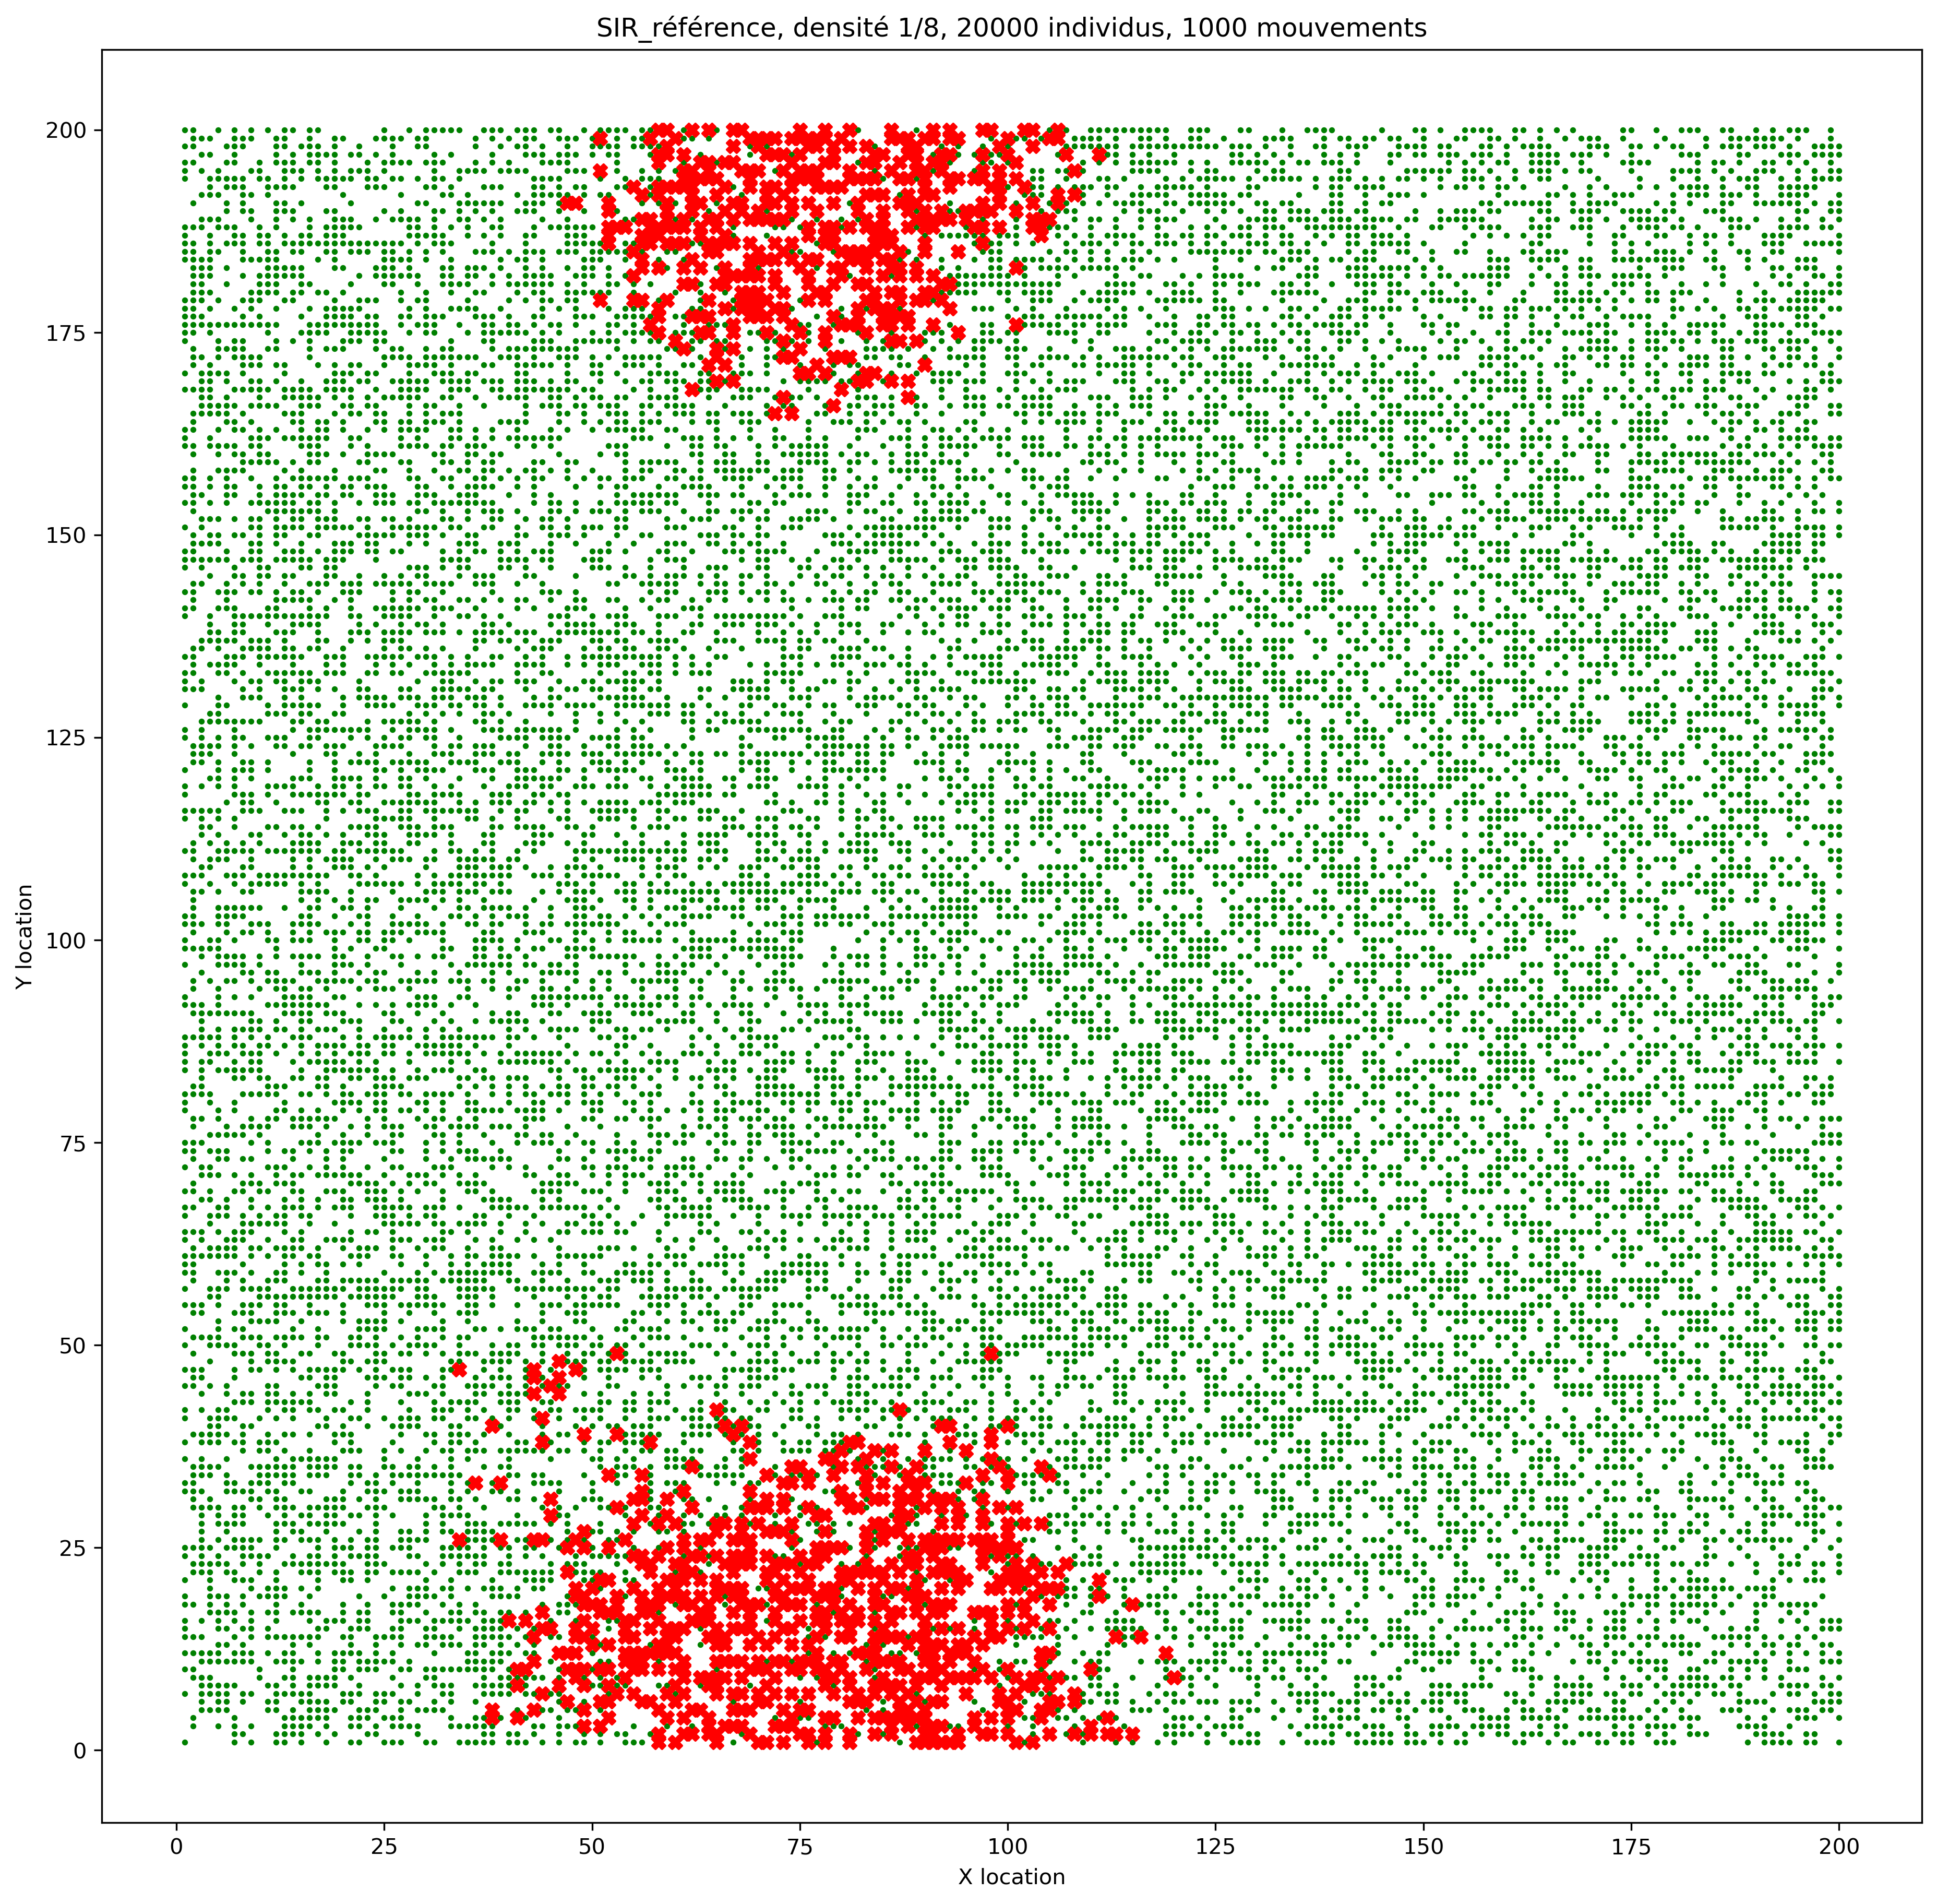
\includegraphics[width=.4\textwidth]{Images/SIR_position_2_20.png}
	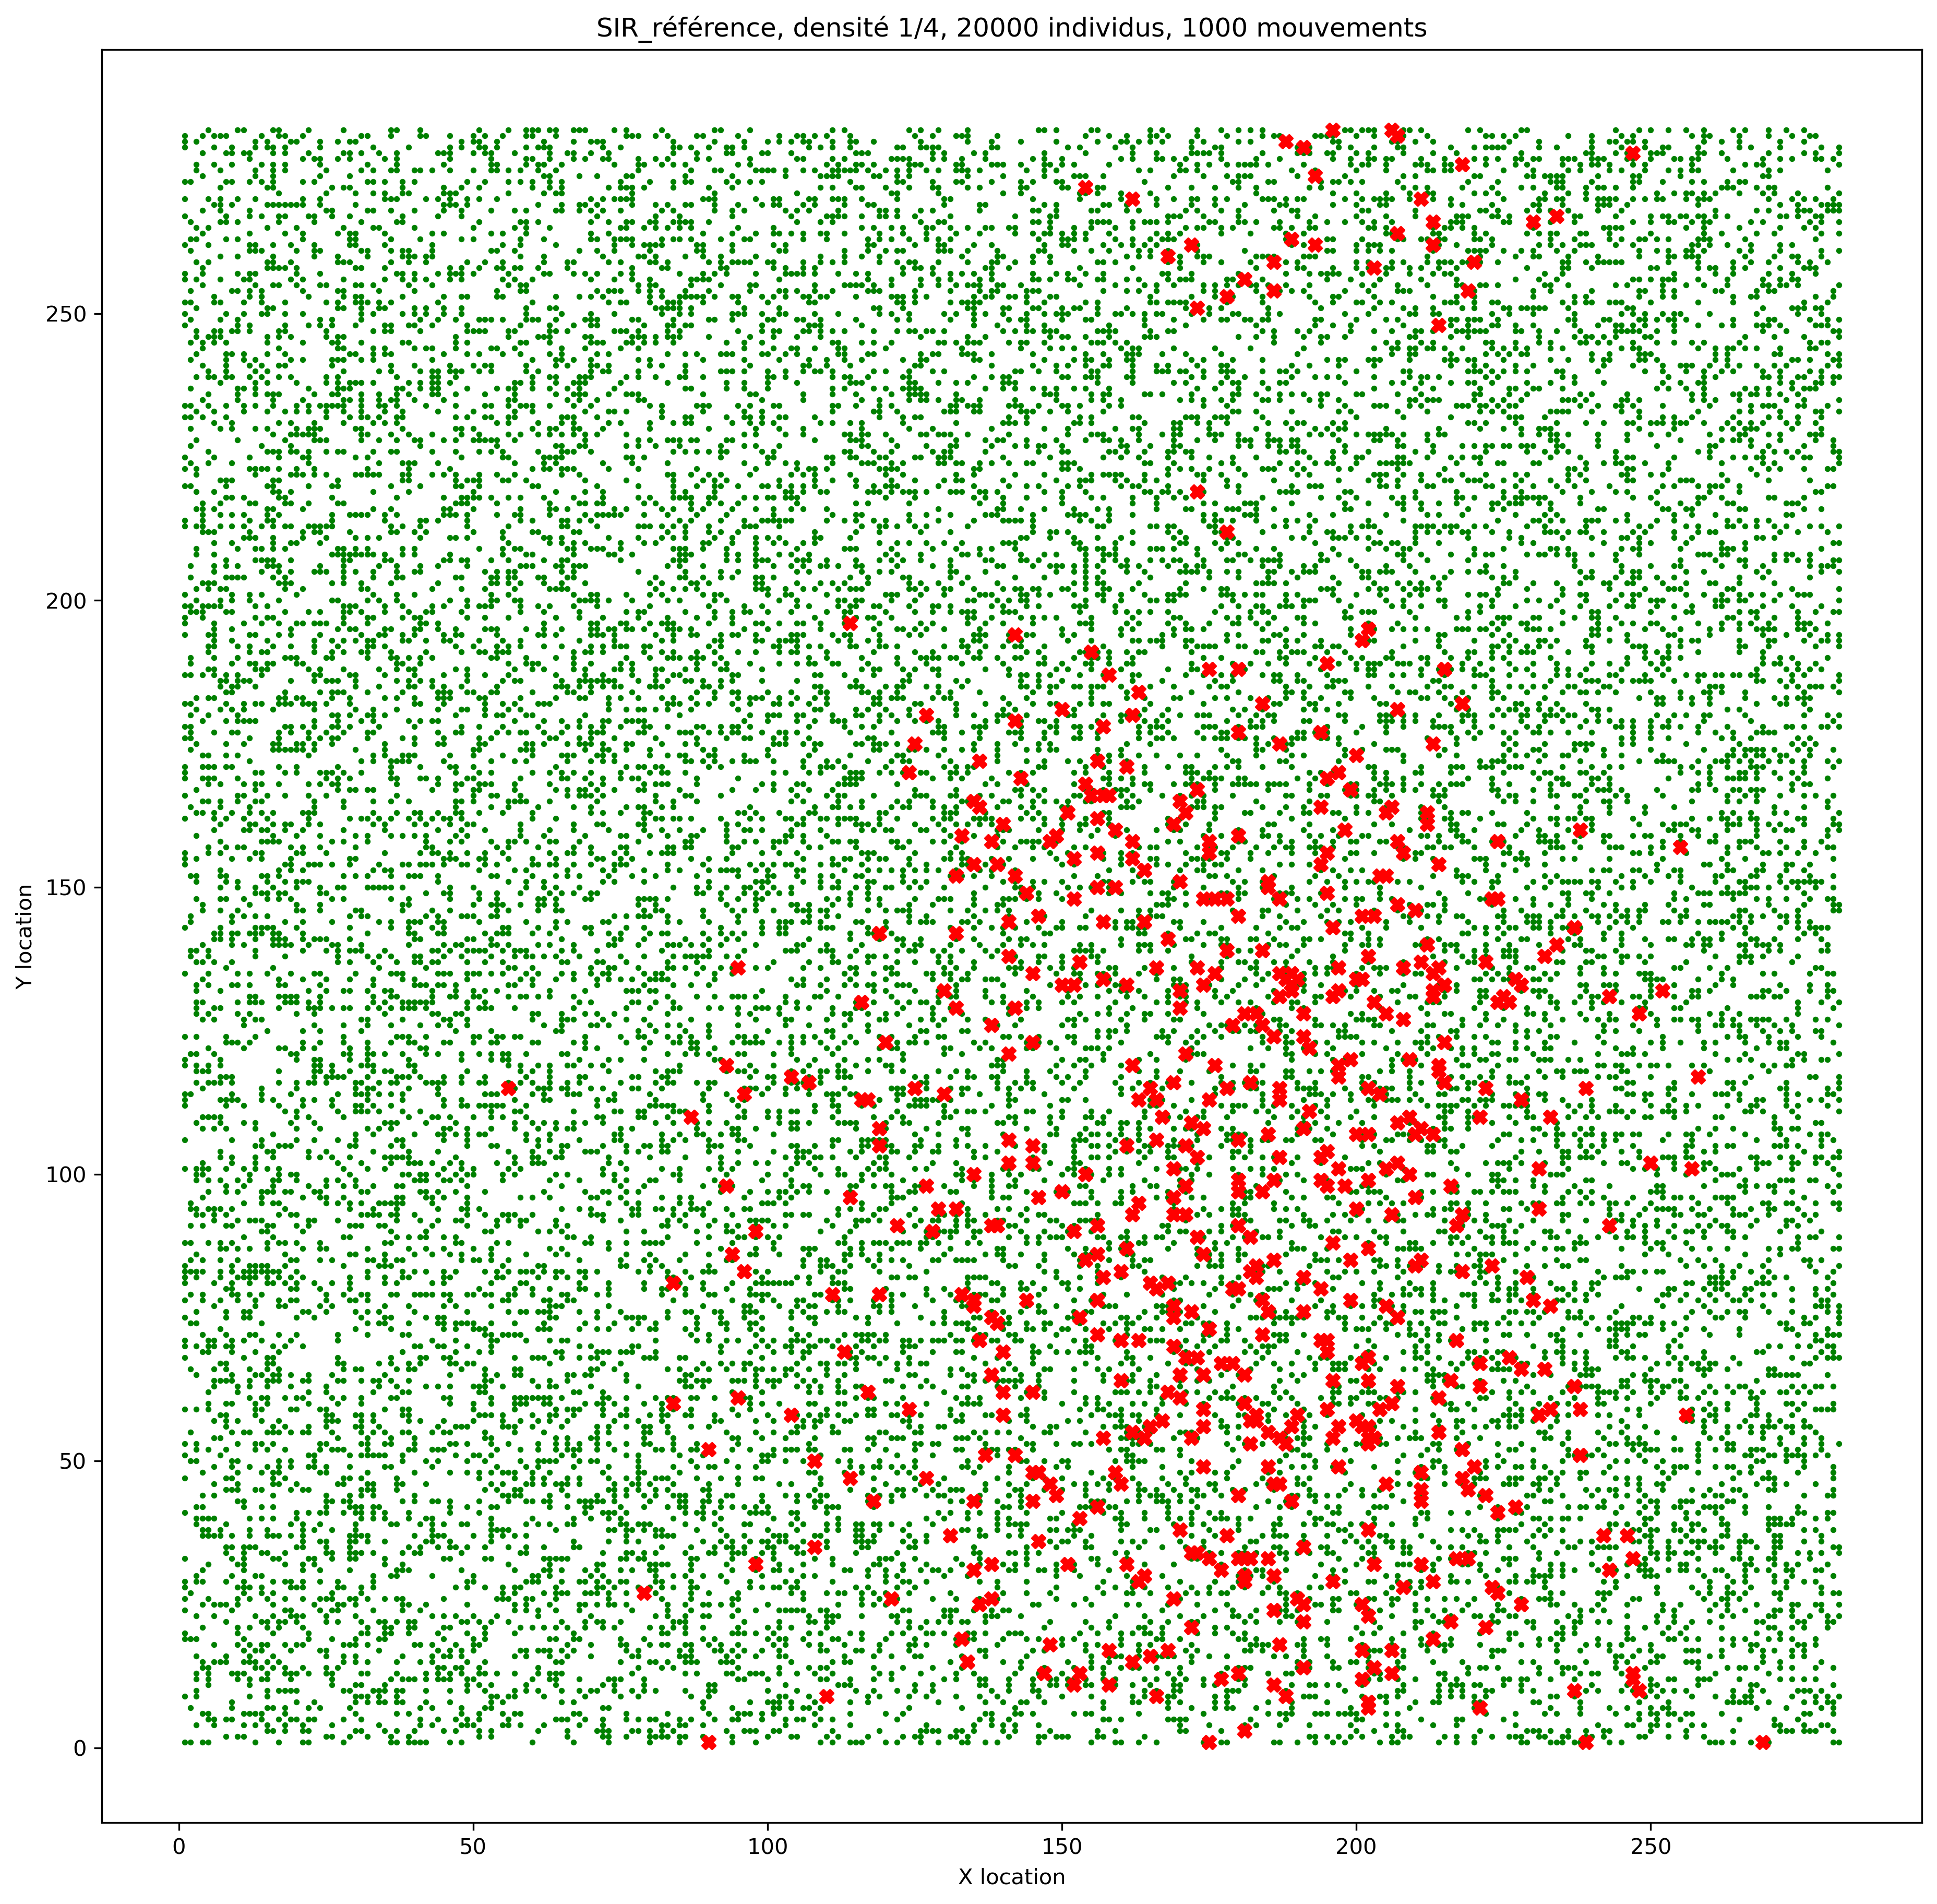
\includegraphics[width=.4\textwidth]{Images/SIR_position_4_20.png}
	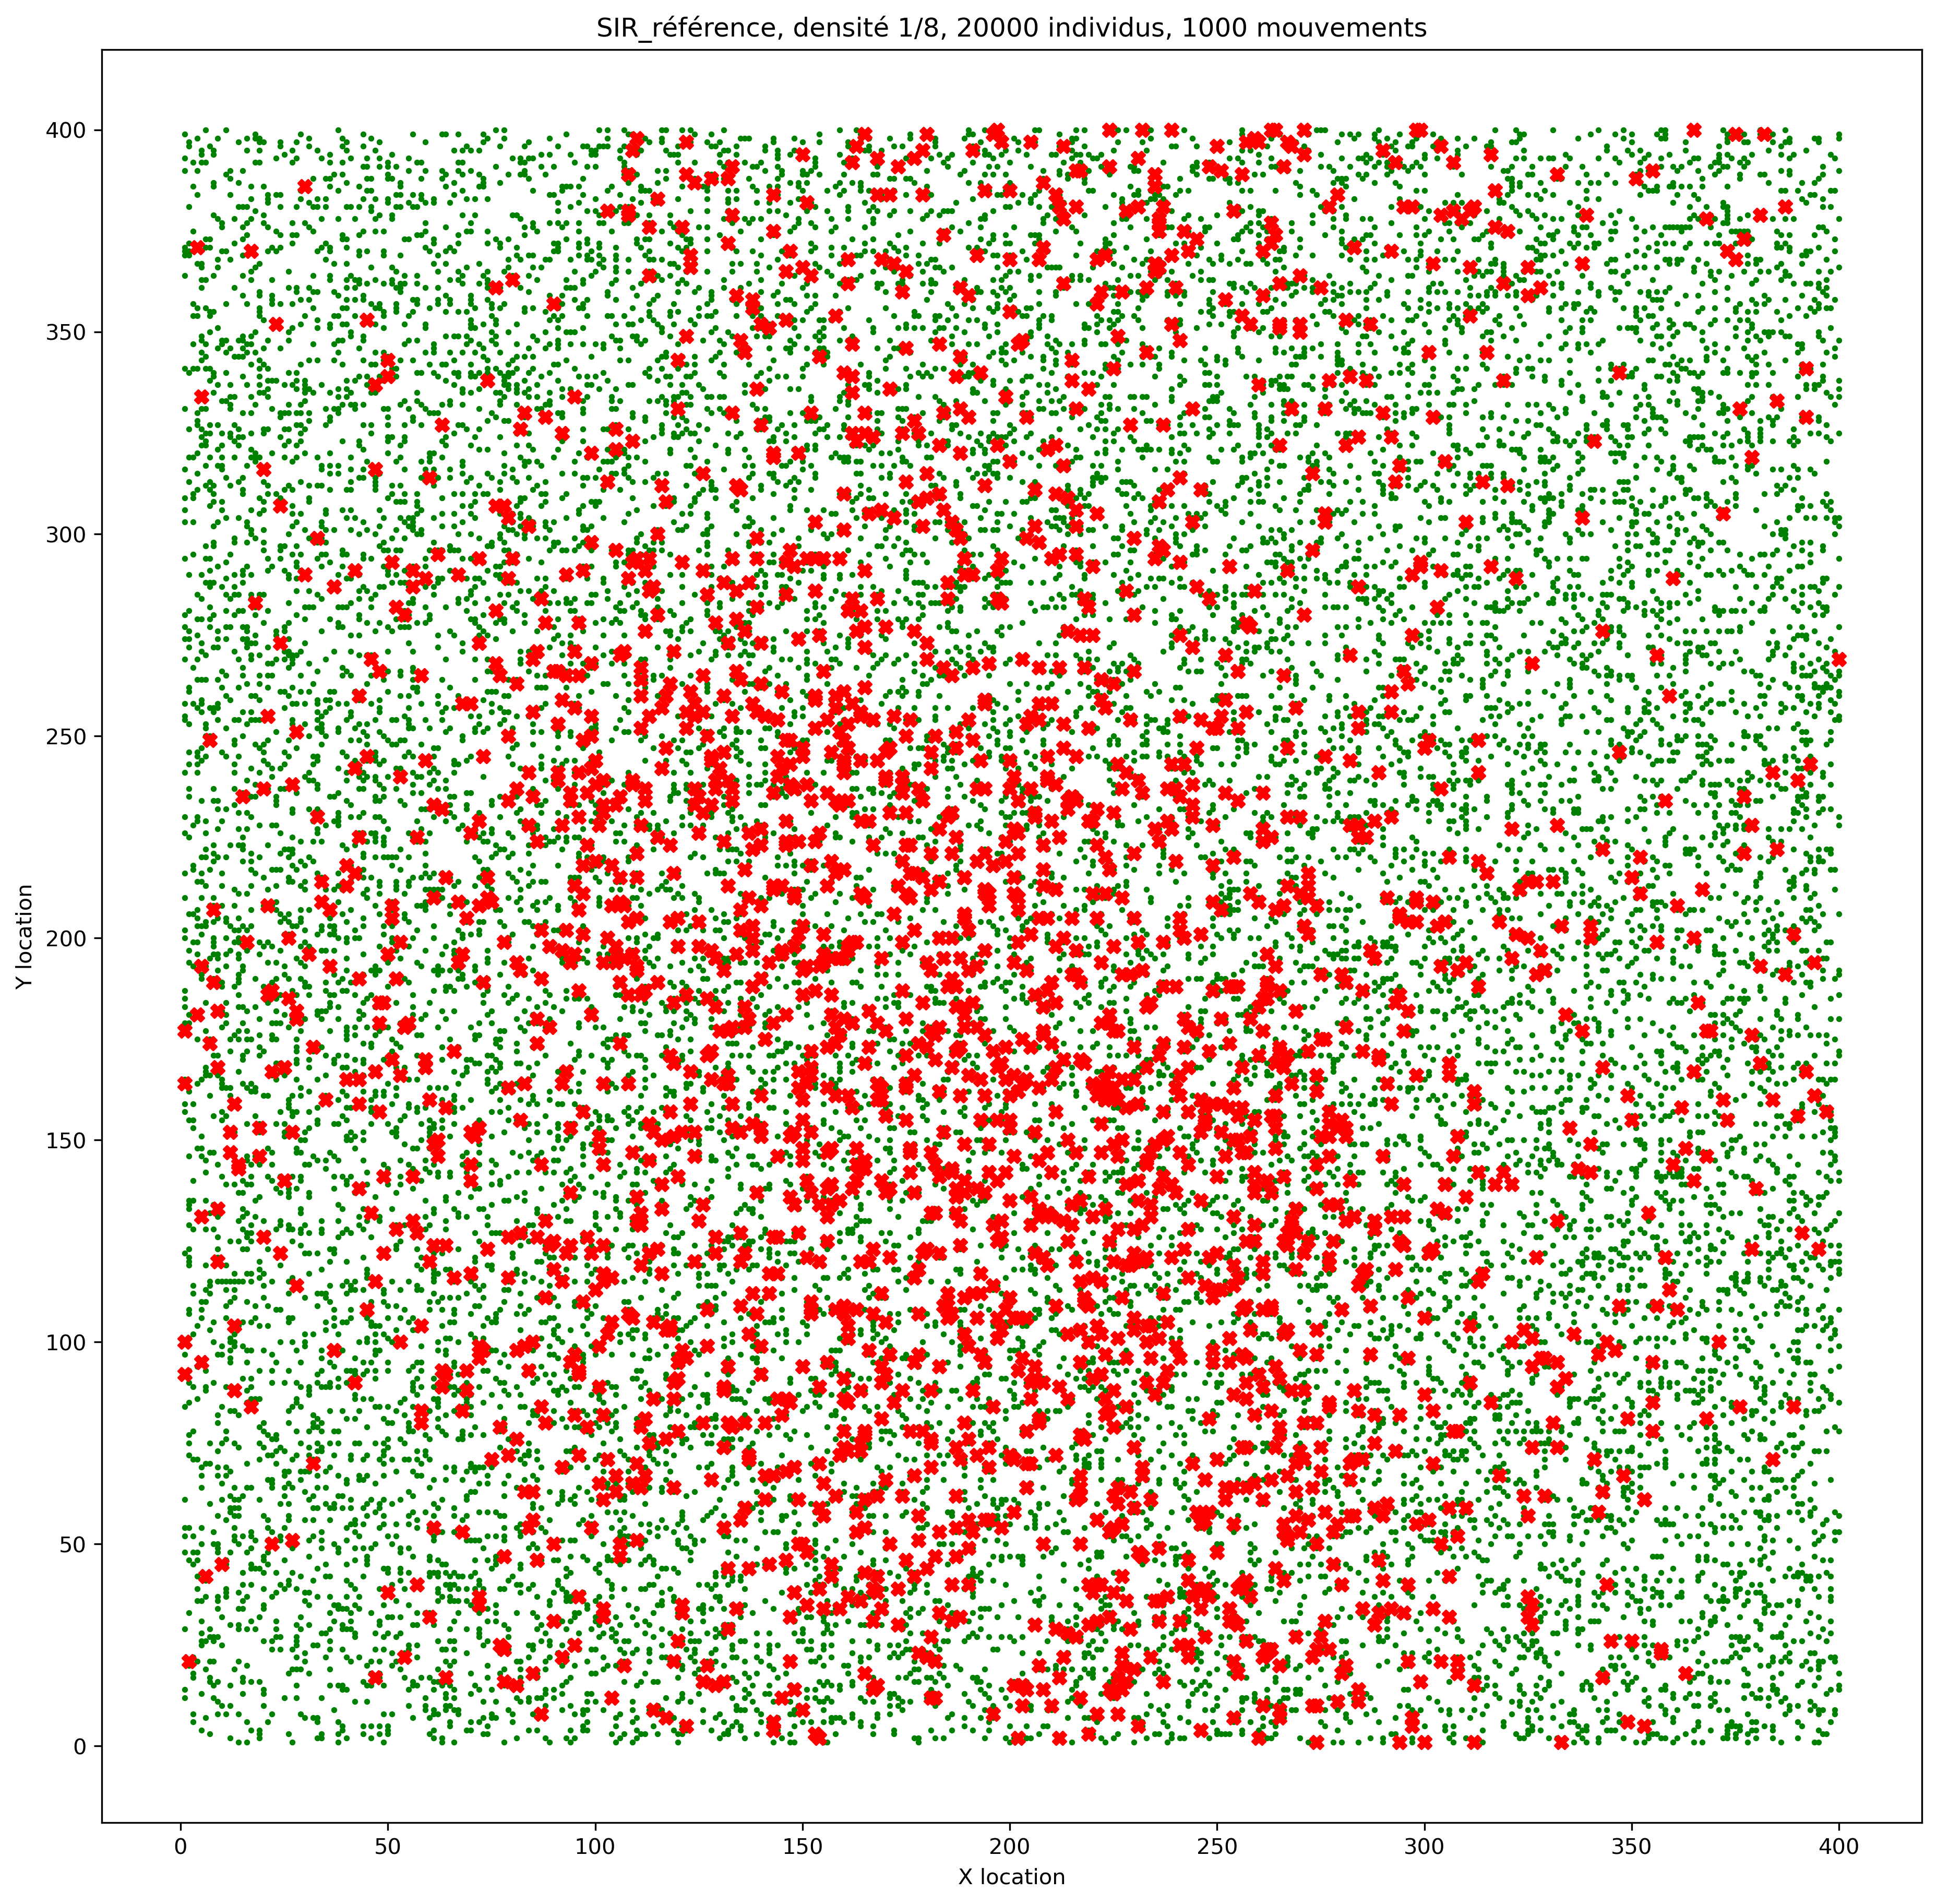
\includegraphics[width=.4\textwidth]{Images/SIR_position_8_20.png}
	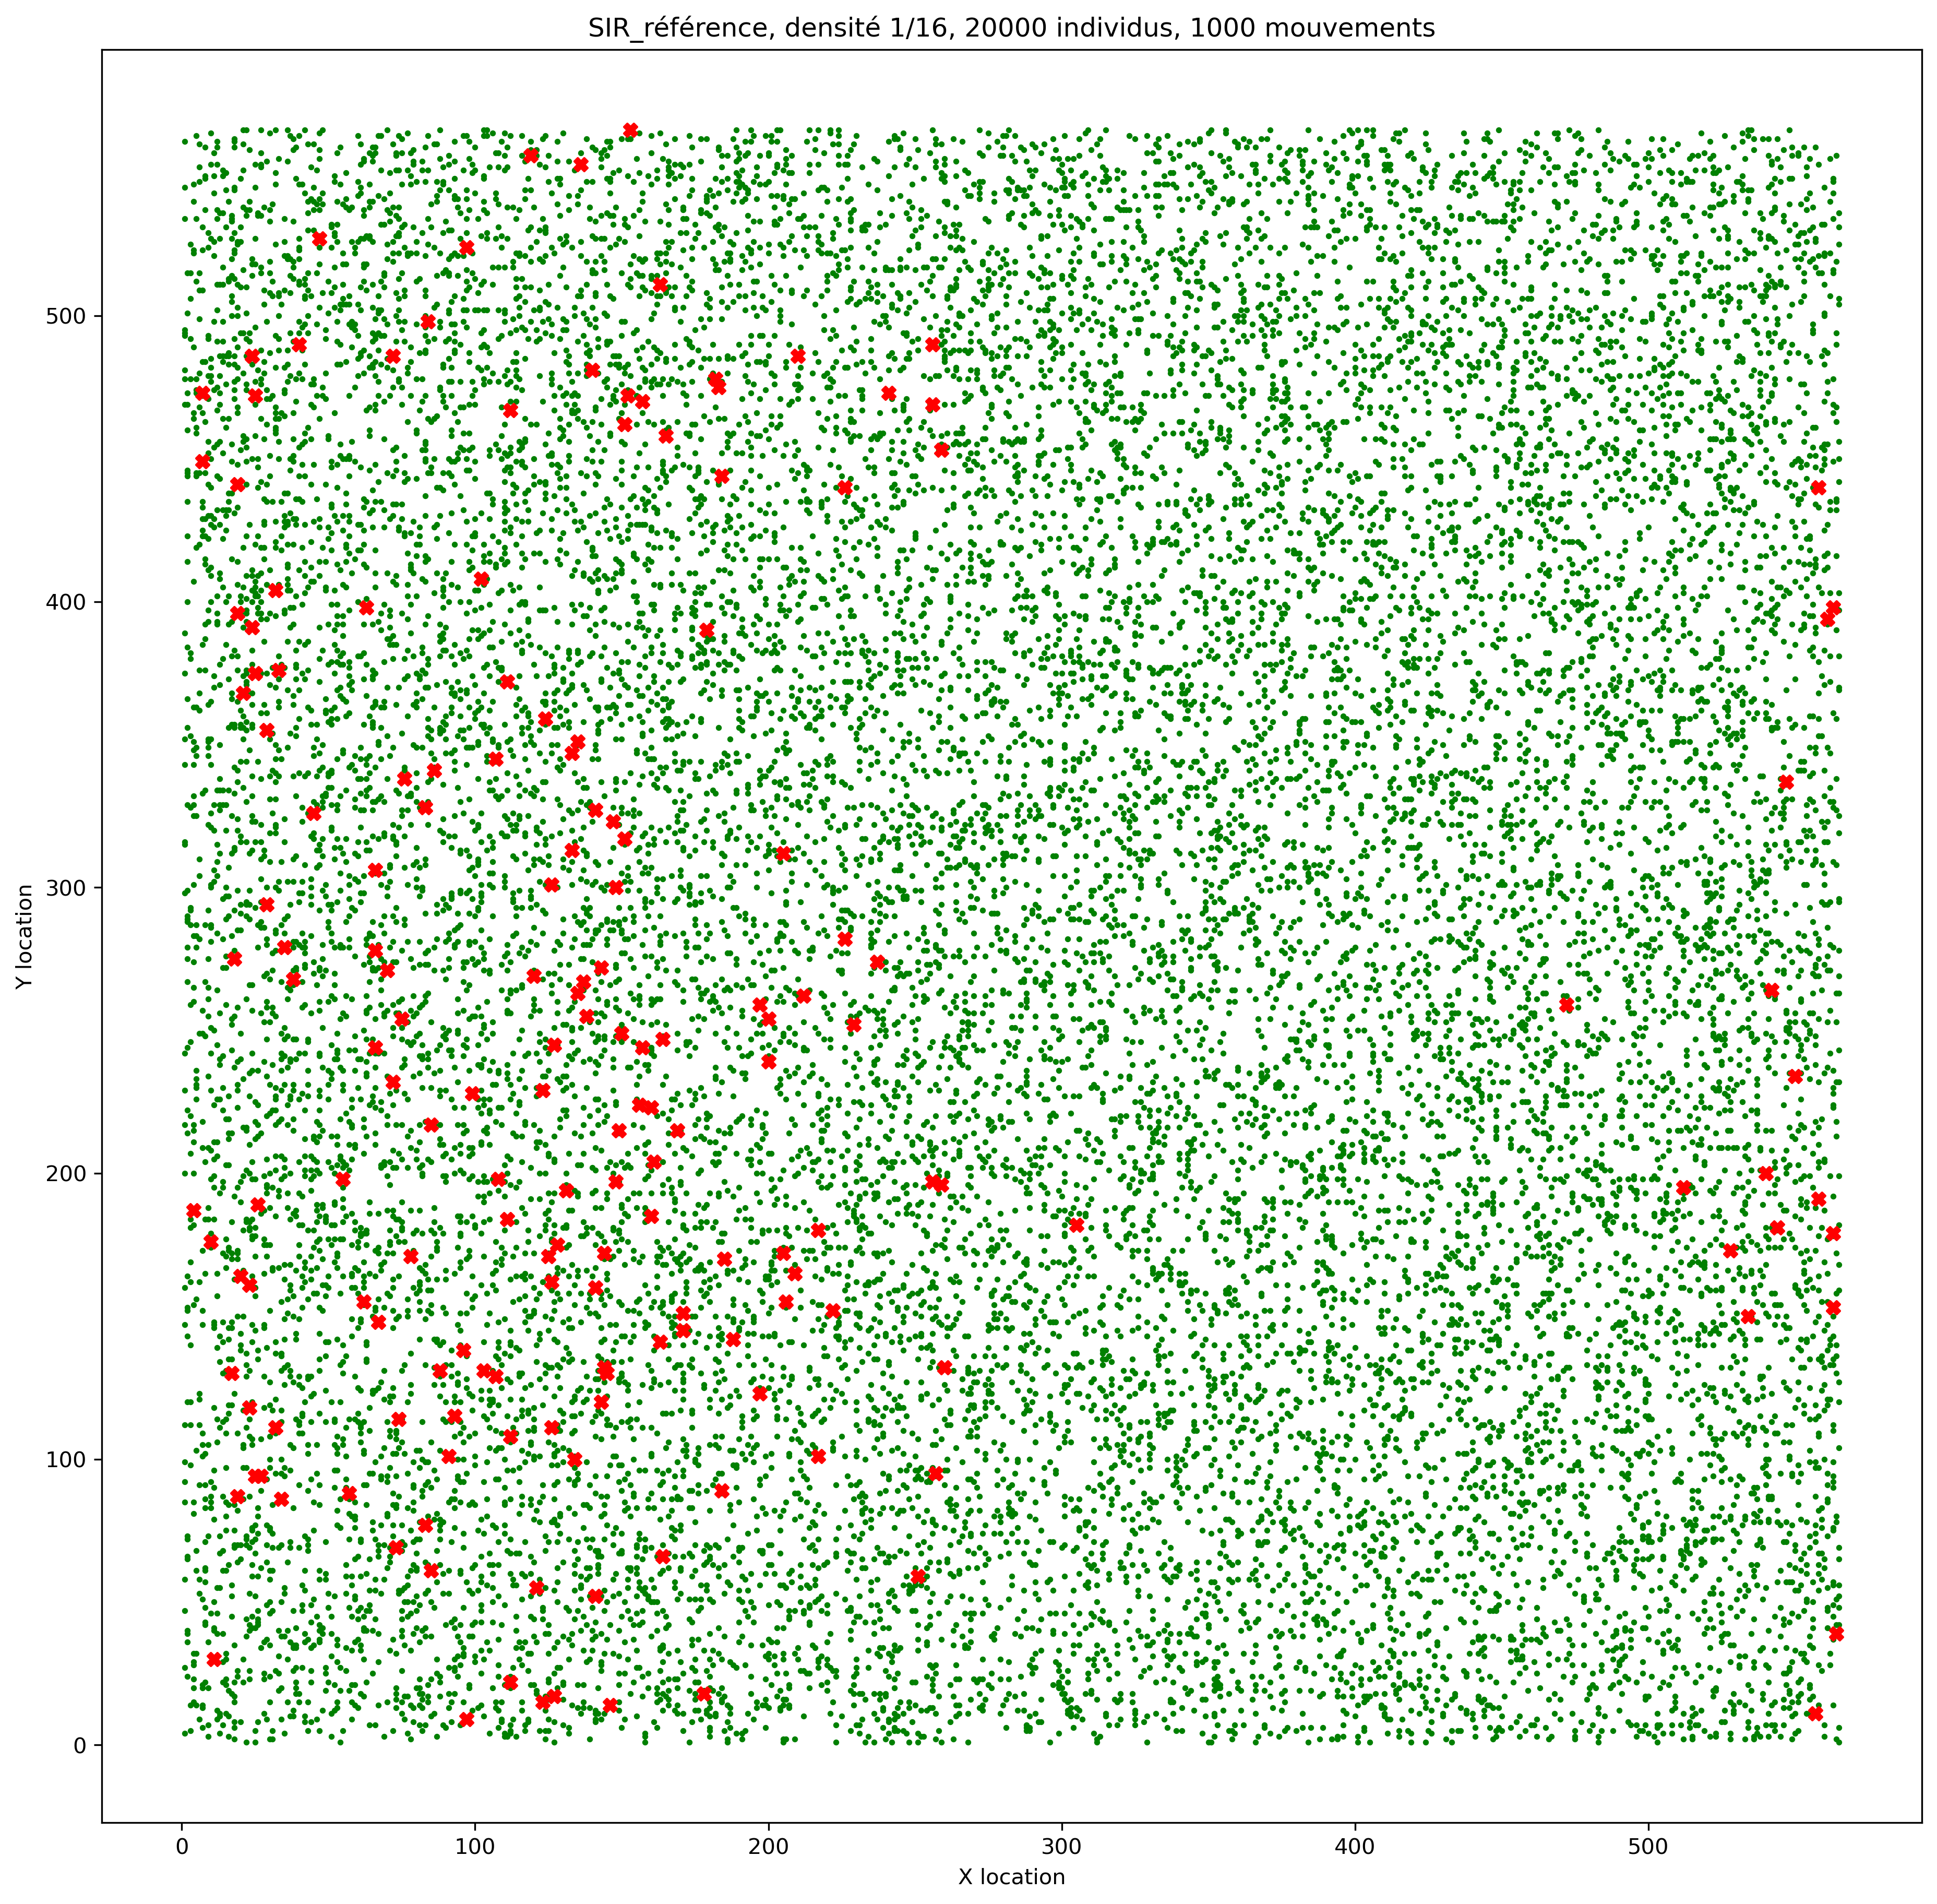
\includegraphics[width=.4\textwidth]{Images/SIR_position_16_20.png}
	\caption{test}
\end{figure}

Modifications à effectuer...

\newpage

\subsection{Variations aléatoires}

Tout comme pour les simulations SI, nous calculons les variations d'une simulation à une autre et ceci pour des paramètres identiques. Les mesures sont faites sur un ensemble de simulations de densité $\frac{1}{8}$ ainsi que $\frac{1}{16}$ avec une population de $20000$ individus.

\begin{figure}[h]
	\centering
	\captionsetup{justification=centering}
	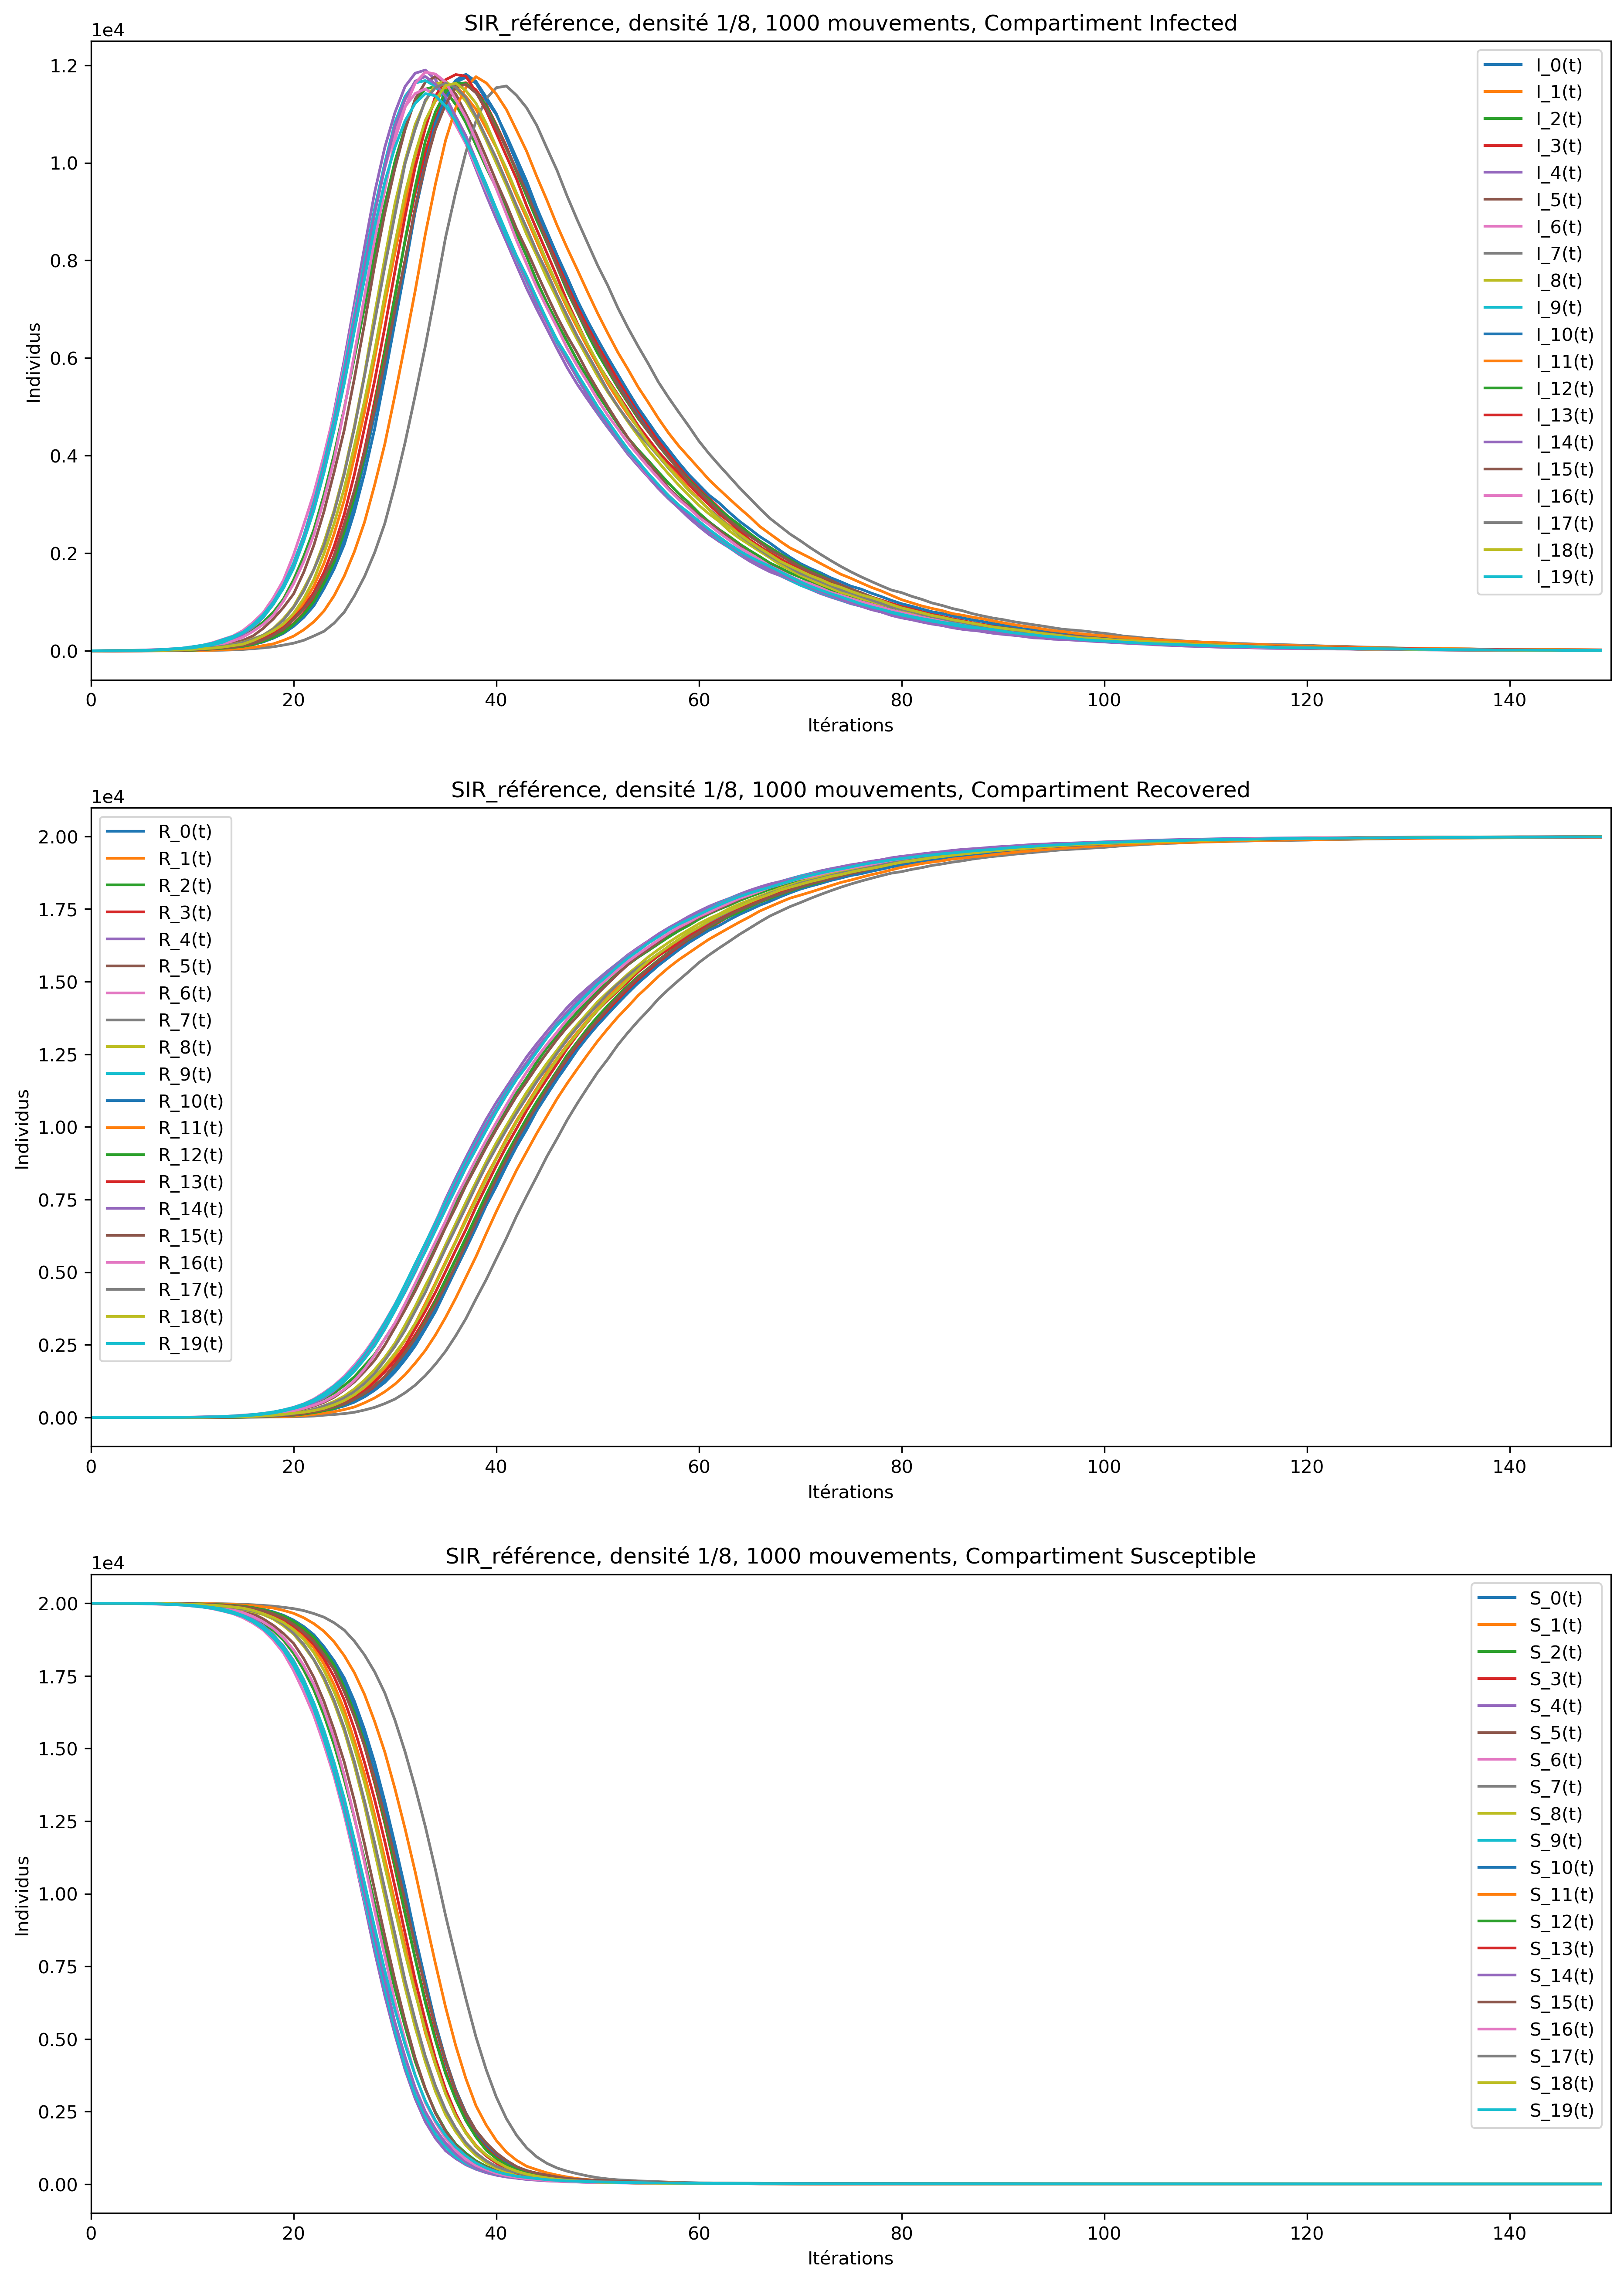
\includegraphics[width=.4\textwidth]{Images/SIR_divergence_8_1000.png}
	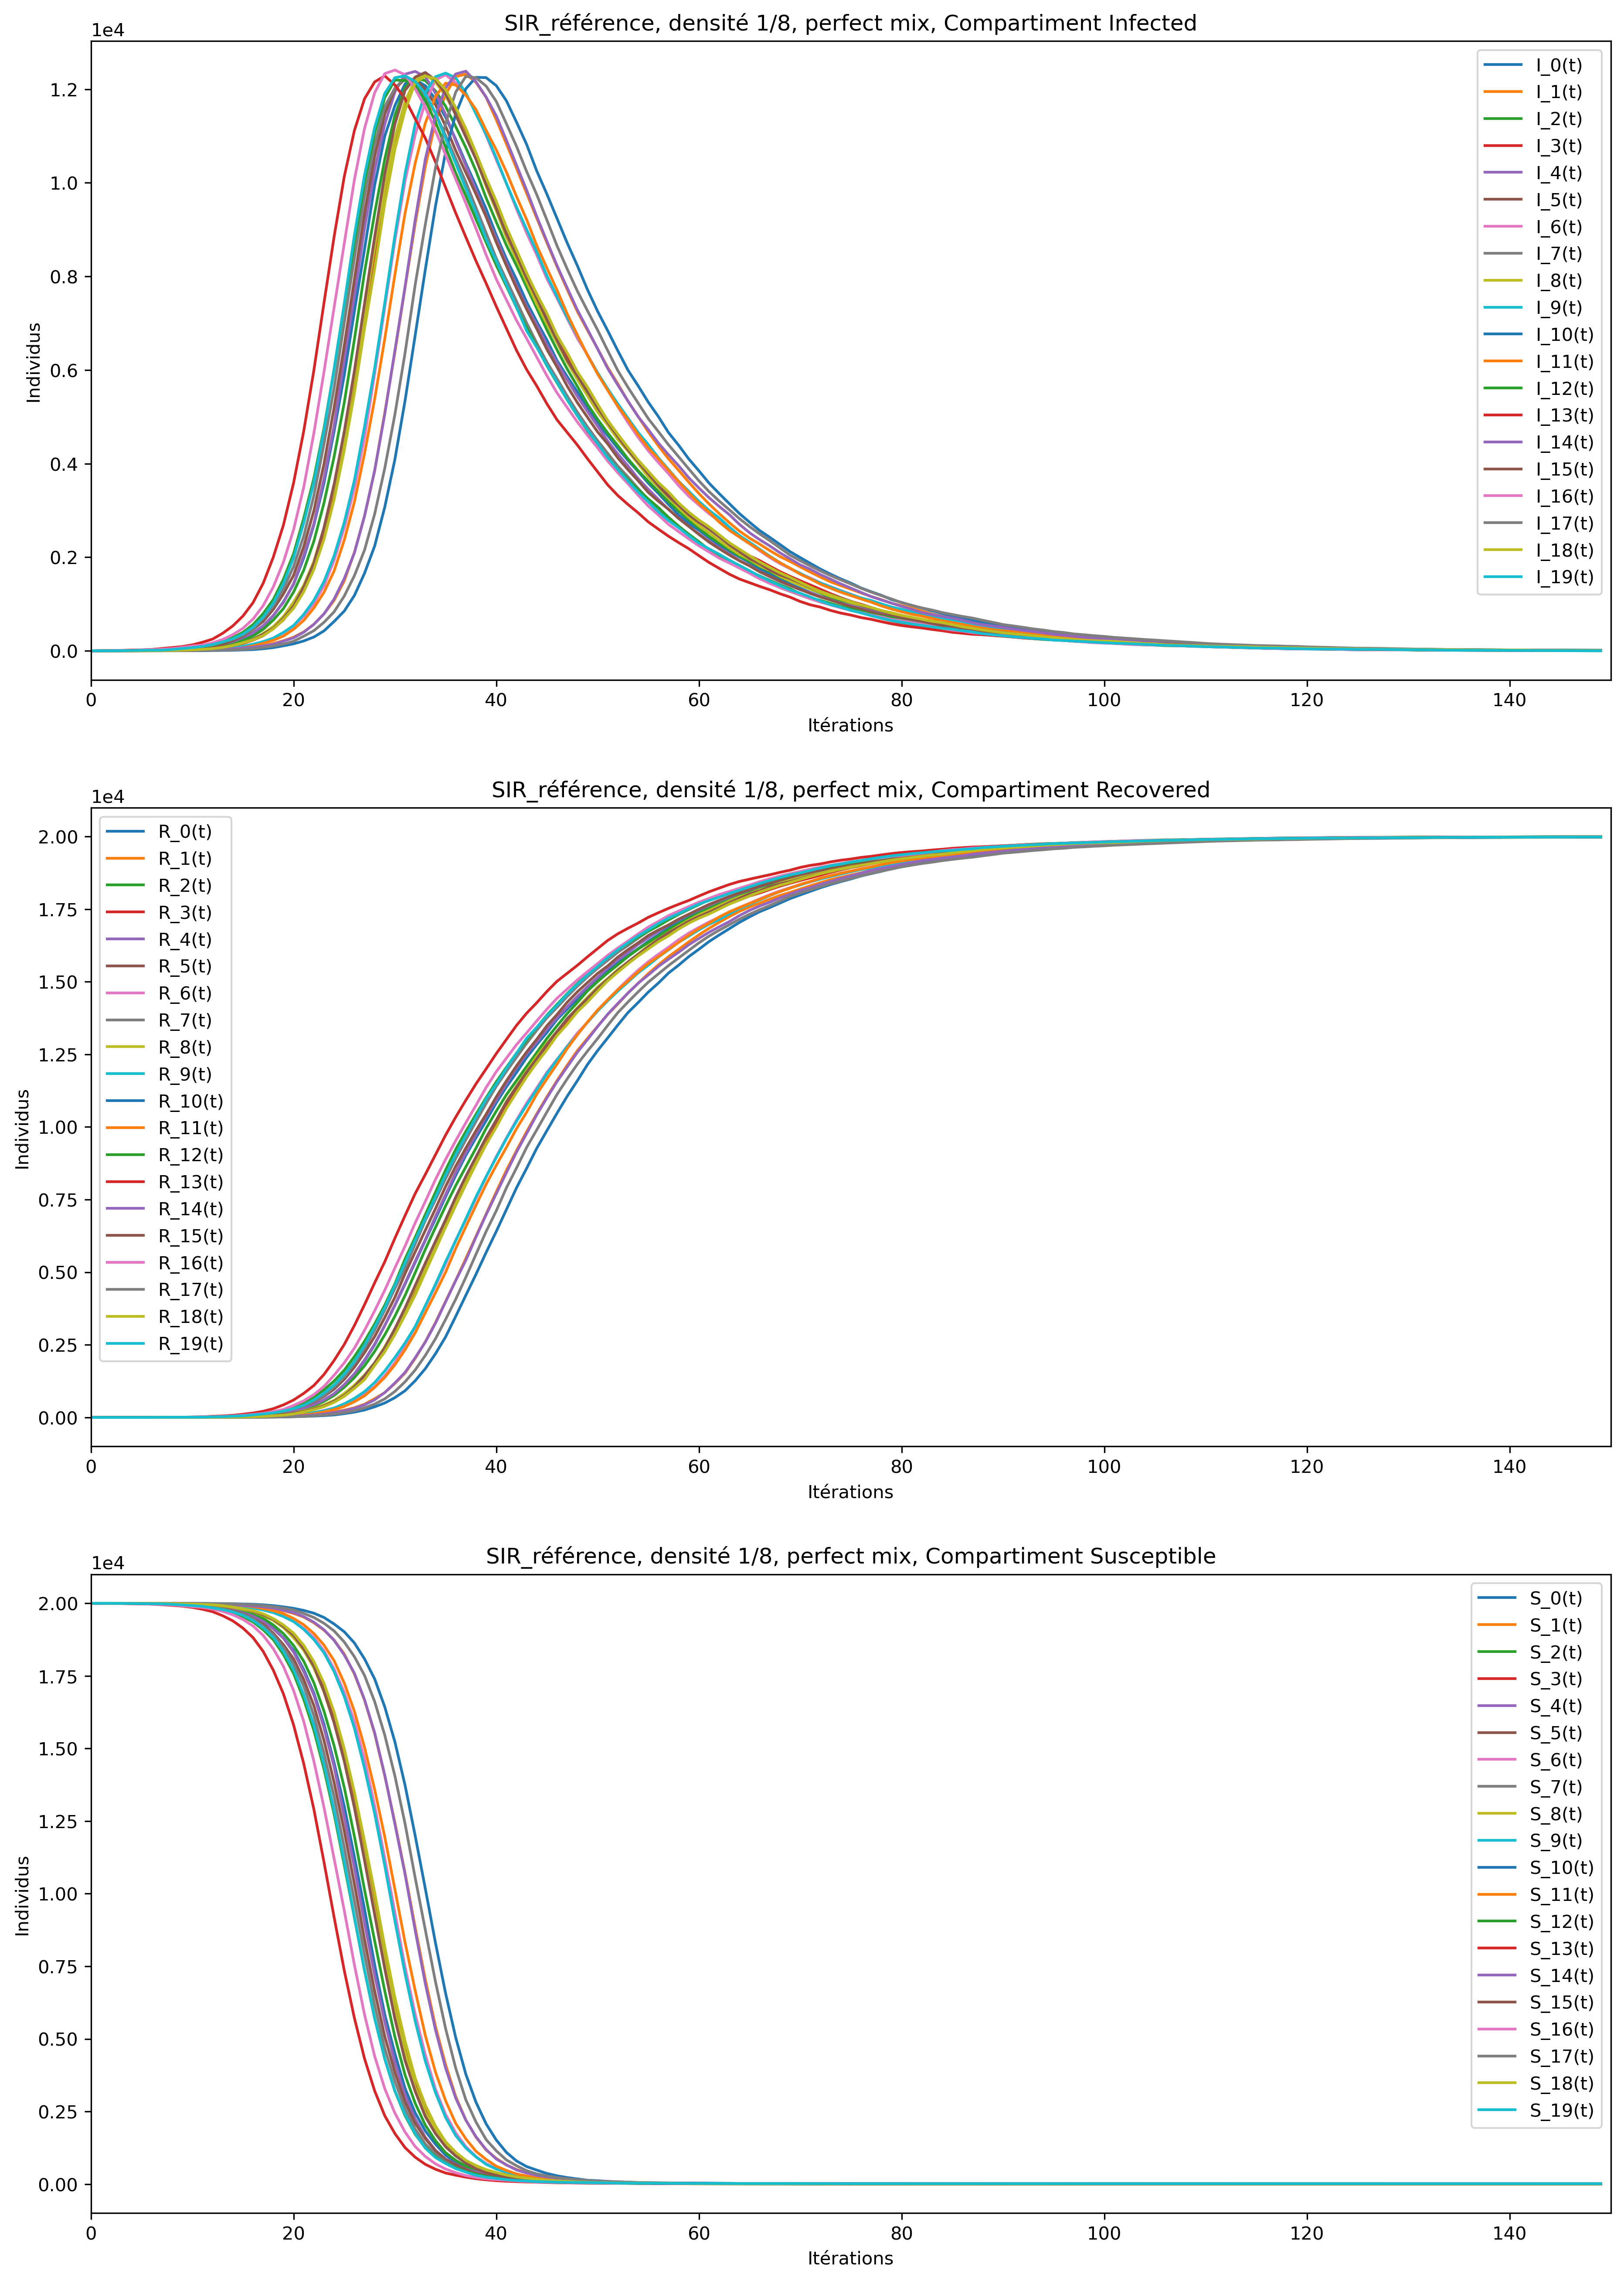
\includegraphics[width=.4\textwidth]{Images/SIR_divergence_8_mix.png}
	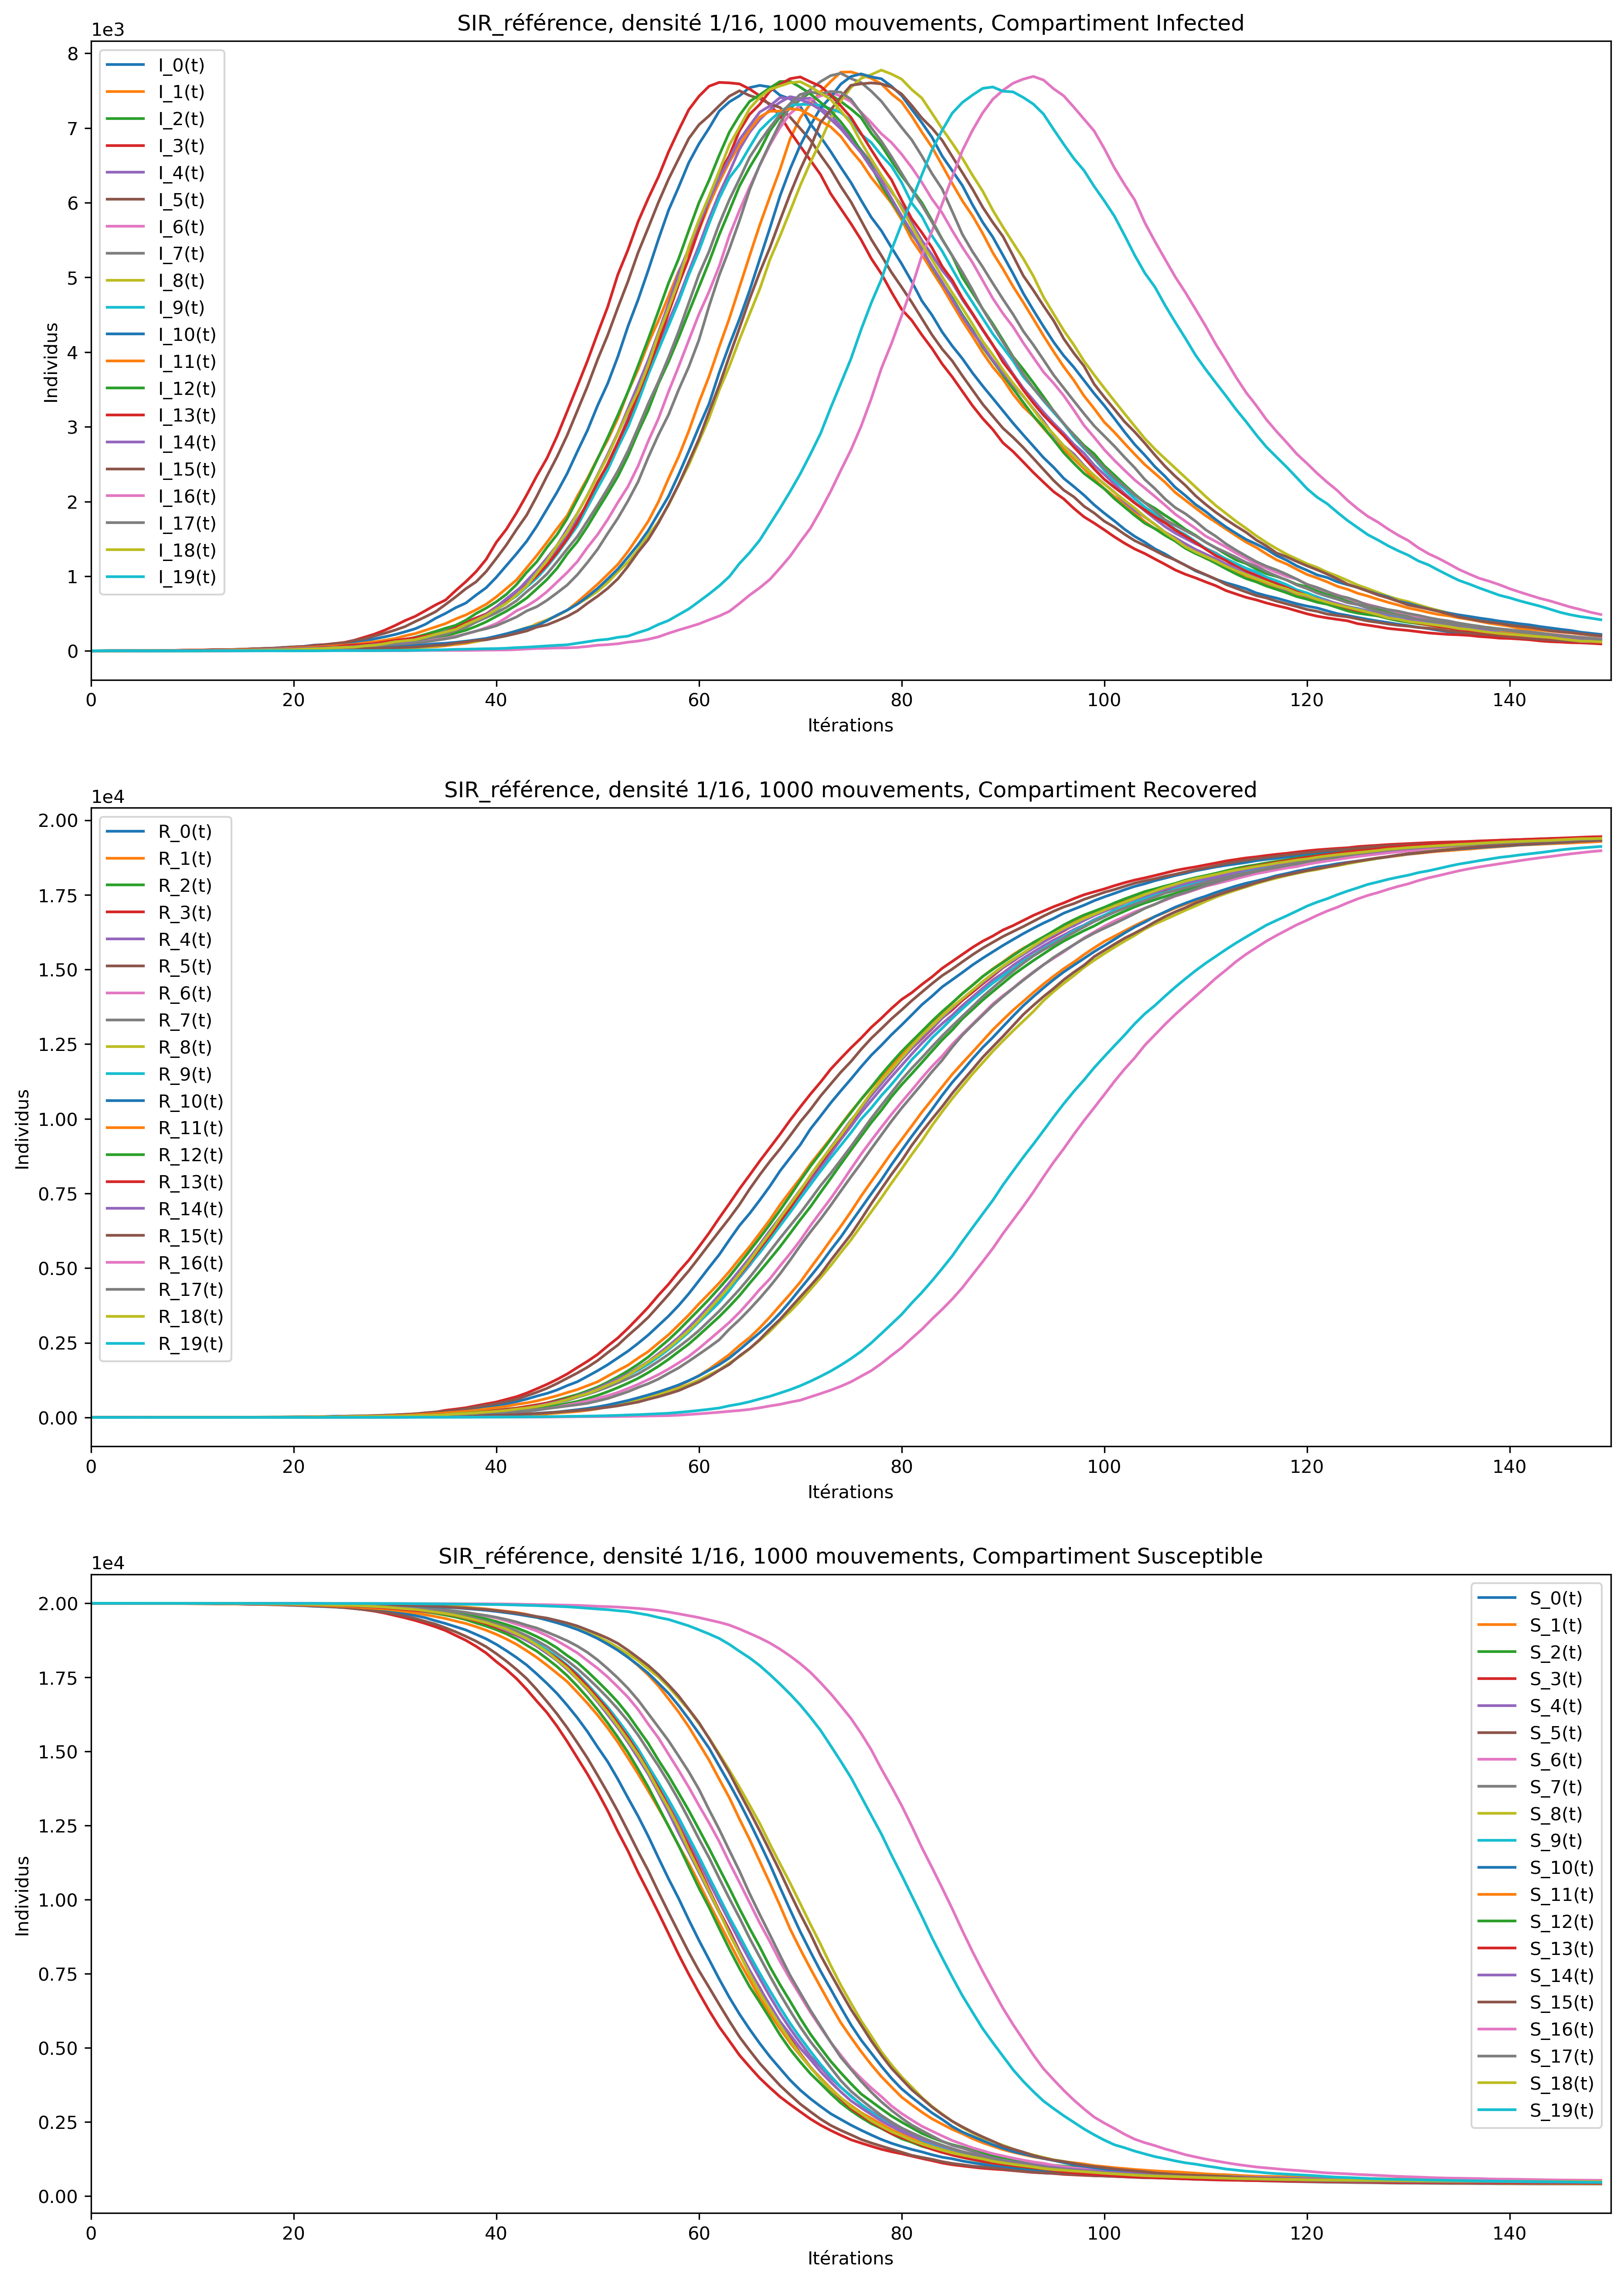
\includegraphics[width=.4\textwidth]{Images/SIR_divergence_16_1000.png}
	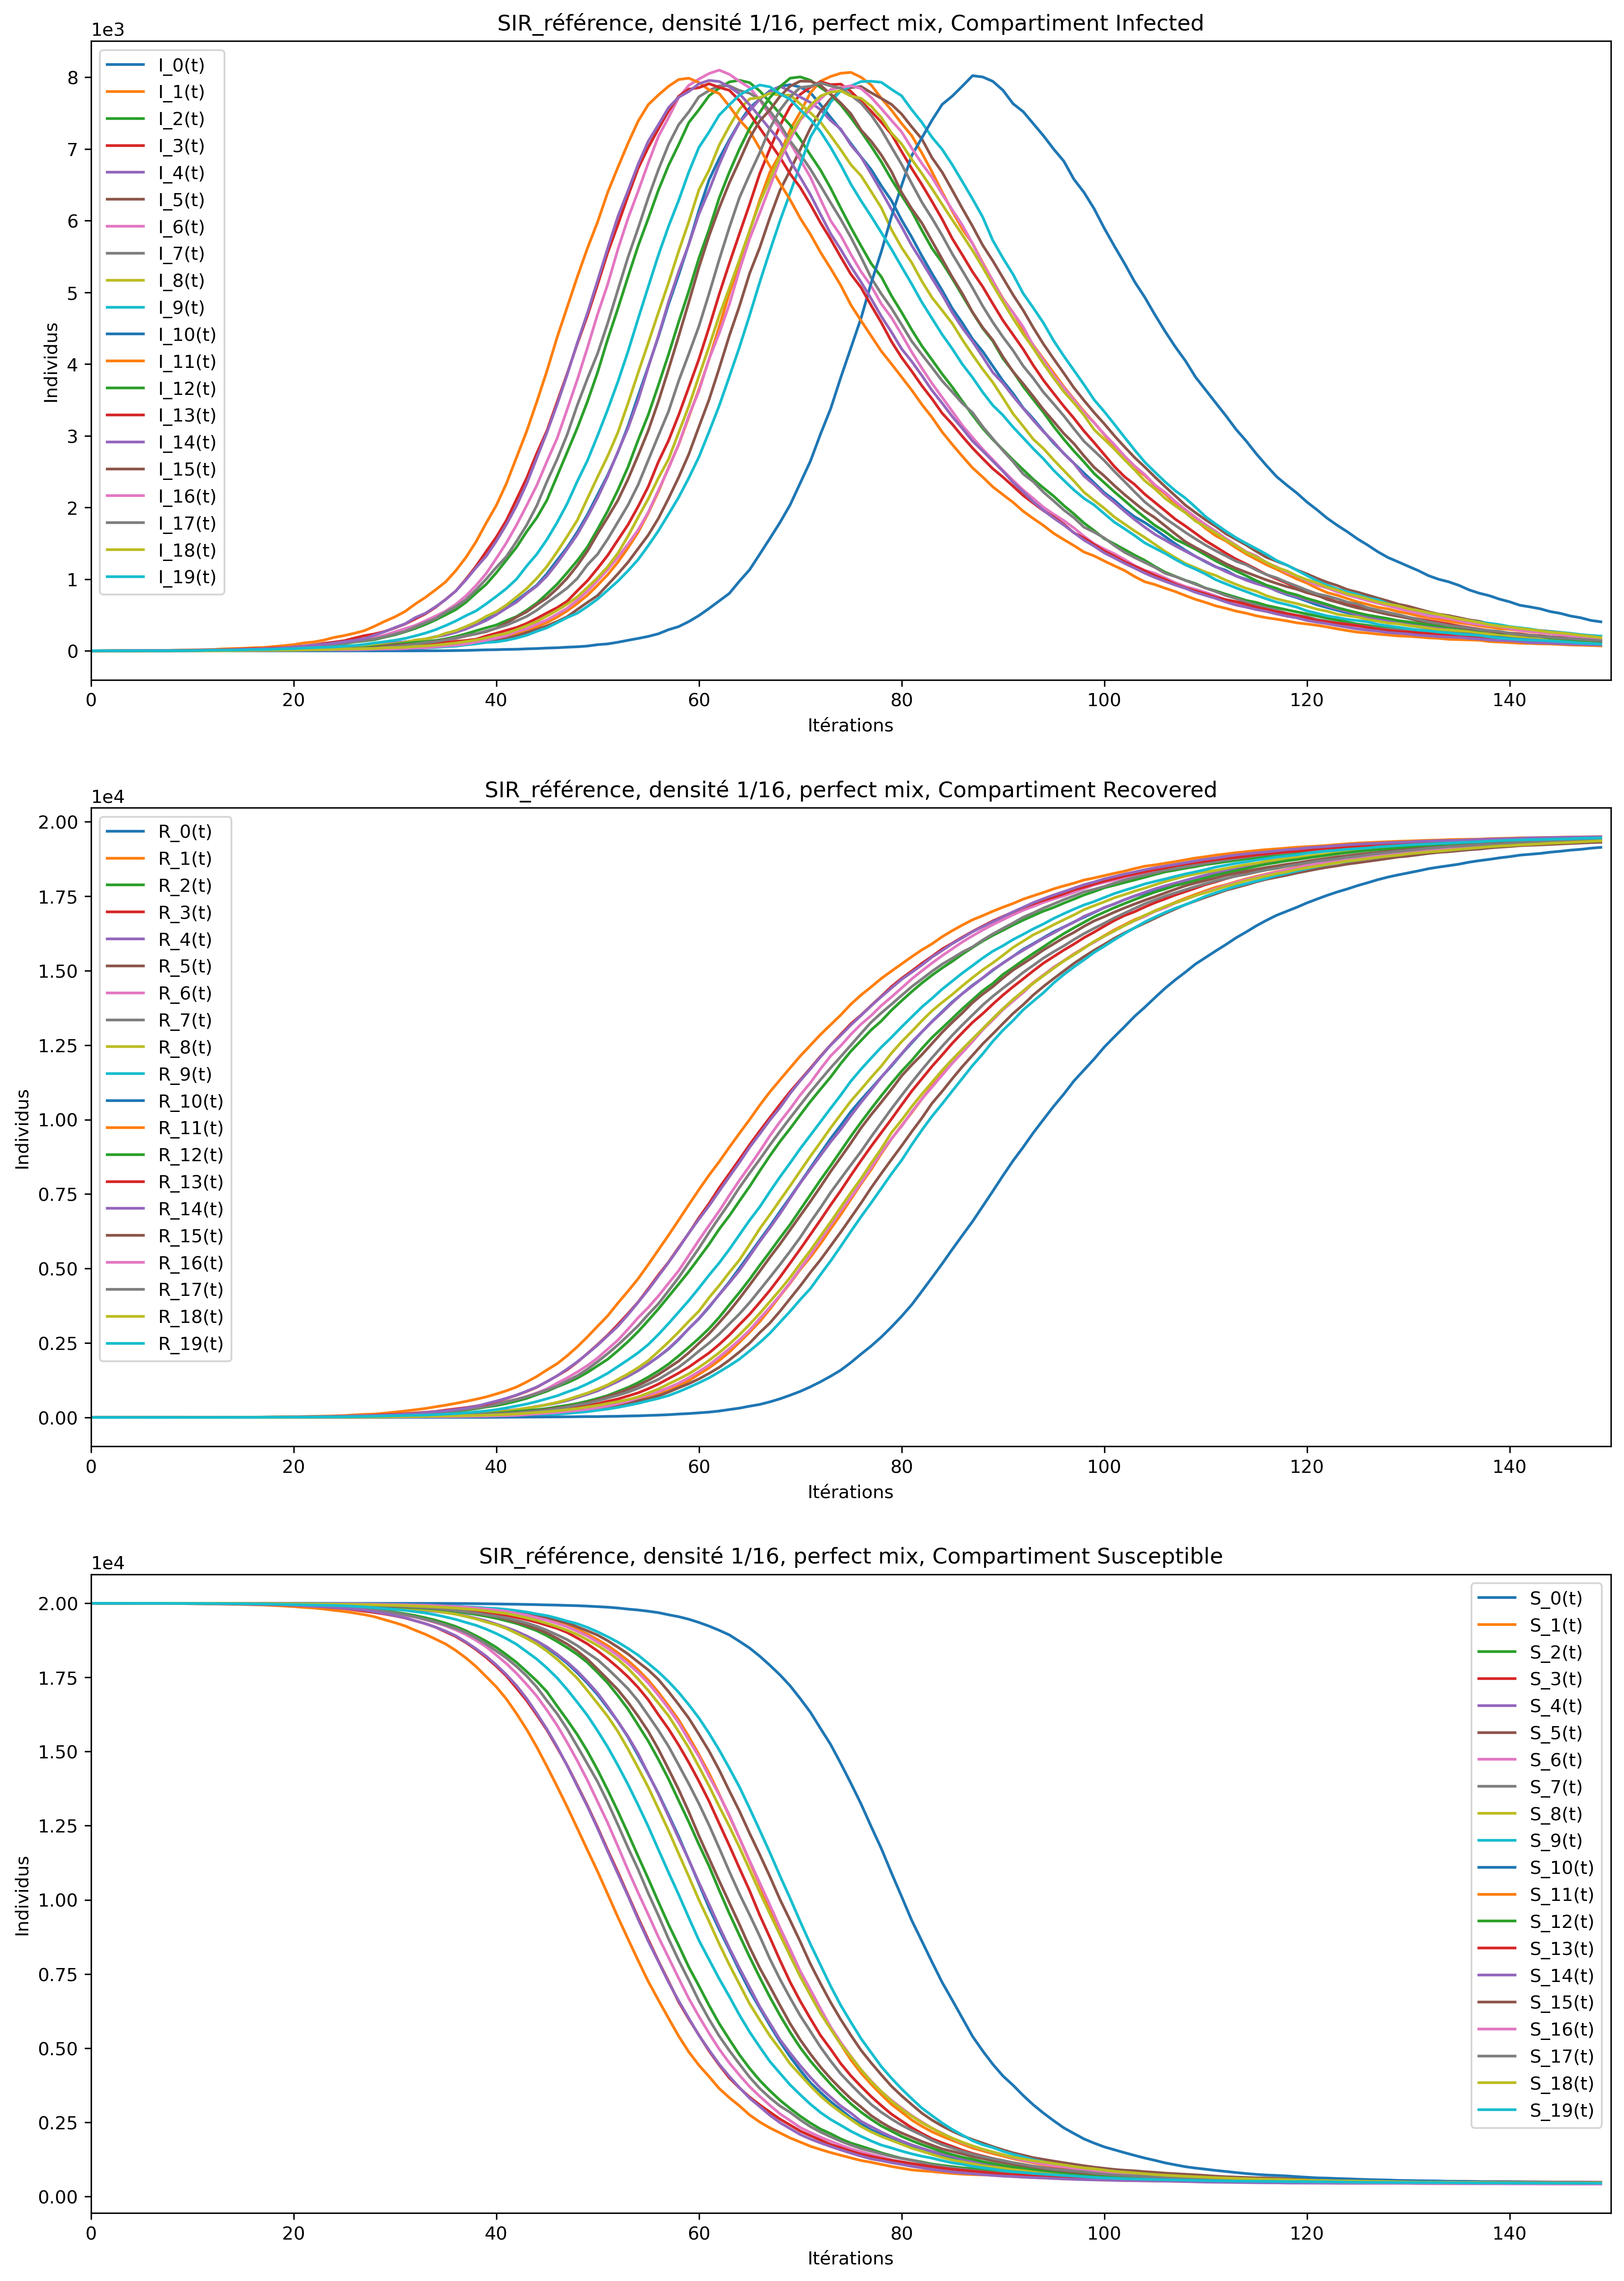
\includegraphics[width=.4\textwidth]{Images/SIR_divergence_16_mix.png}
	\caption{test}
\end{figure}

\begin{table}[H]
	\centering
	\captionsetup{justification=centering}
	\caption[Variations : SIR]{Voisinage : modèle SIR\label{tab:grid}}
	\begin{tabular}{@{\extracolsep{\fill} } c|| c| c| c| c|}
	 & \multicolumn{2}{|c|}{1000 mouvements} & \multicolumn{2}{|c|}{Mélange parfait} \\
	\midrule
	\midrule
	densité & 1/8 & 1/16 & 1/8 & 1/16\\
	\midrule
	min & $33$ & $62$ & $29$ & $59$\\
	\midrule
	max & $41$ & $93$ & $38$ & $87$\\
	\midrule
	mean & $35.35$ & $72.85$ & $33.2$ & $69.35$\\
	\midrule
	std & $2.10$ & $7.28$ & $2.58$ & $6.77$\\
	\bottomrule
	\end{tabular}
	\end{table}

\subsection{Latence des simulations}

\subsection{Mouvements variable}

\begin{figure}[h]
	\centering
	\captionsetup{justification=centering}
	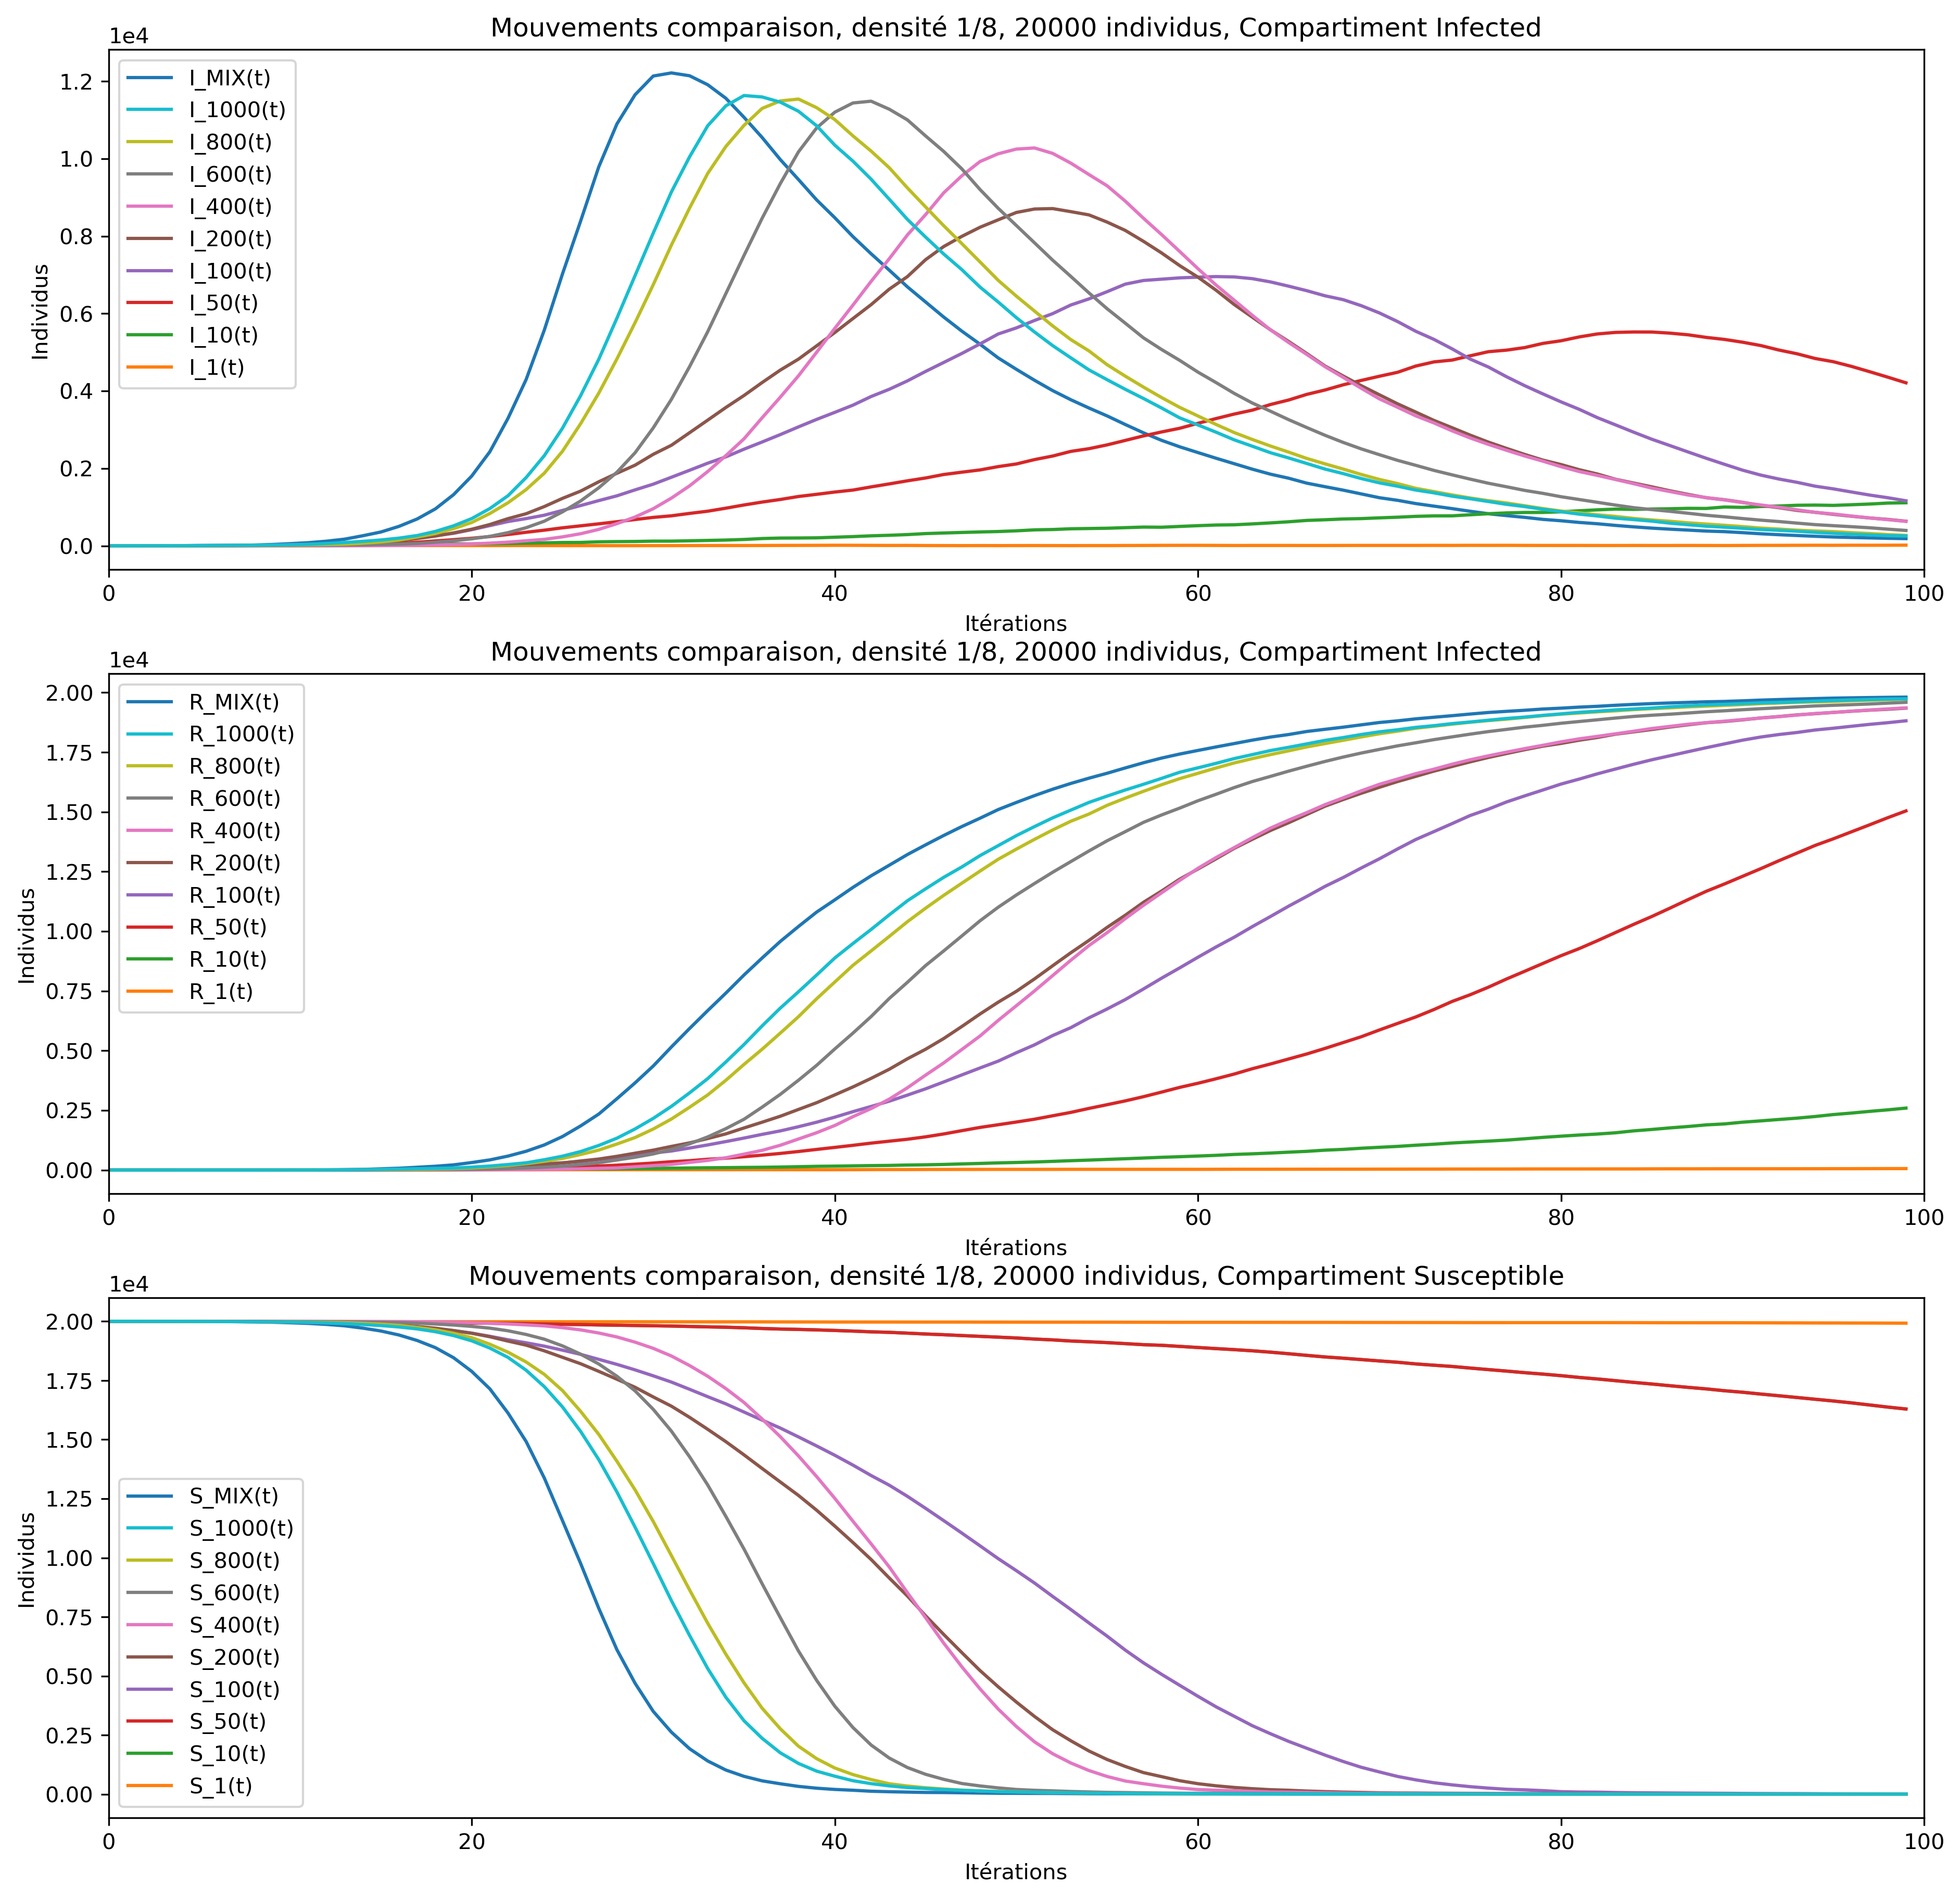
\includegraphics[width=.7\textwidth]{Images/SIR_mouvements_variables.png}
	\caption{test}
\end{figure}

\subsection{Comparaison 1000 mouvements}


